

\renewcommand\chapterillustration{./Chapter_Image}
\renewcommand\chapterwhat{ }
\renewcommand\chapterbecause{ }
\chapter{Probabilidade}

\mbox{}\thispagestyle{empty}\clearpage

\thispagestyle{empty}

\begin{center}
Projeto: LIVRO ABERTO DE MATEMÁTICA

\noindent \begin{tabular}{lcccr}
\includegraphics[scale=.15]{impa}& \quad\quad& \includegraphics[width=3cm]{logo} & \quad\quad& \includegraphics[scale=.24]{obmep} 
\end{tabular}
\end{center}

\vspace*{.3cm}

Cadastre-se como colaborador no site do projeto: \url{umlivroaberto.com}

Versão digital do capítulo:

\url{https://www.umlivroaberto.org/BookCloud/Volume_1/master/view/PE511.html}

\begin{center}
  \includegraphics[width=2cm]{canvas}
\end{center}

\begin{tabular}{p{.15\textwidth}p{.7\textwidth}}
Título: & Probabilidade\\
Ano/ Versão: & 2019 / versão 0.9 de 05 de junho de 2019\\
Editora & Instituto Nacional de Matem\'atica Pura e Aplicada (IMPA-OS)\\
Realização:& Olimp\'iada Brasileira de Matem\'atica das Escolas P\'ublicas (OBMEP)\\
Produção:& Livro Aberto\\
\\
Coordenação do projeto: & Fabio Simas e Augusto Teixeira (livroaberto@impa.br)\\
\\
  Autores: & Flávia Landim (coordenadora da equipe - UFRJ),\\
        & Alexandre Silva (UNIRIO),\\
        & Nei Rocha (UFRJ),\\
             & Vanessa Matos (SEduc Angras dos Reis e Mesquita).\\
\\
Revisora: &  Cydara Ripoll  \\
\\
Design: & Andreza Moreira (Tangentes Design) \\
\\
  Ilustrações: & --- \\ 
\\
Gráficos: & Beatriz Cabral e Tarso Caldas (Licenciandos da UNIRIO)\\
\\
  Capa: & Foto de --- , no Unsplash \\

\end{tabular}
\vspace{.5cm}


\begin{minipage}[l]{5cm}
  \includegraphics[width=3.5cm]{cc-by-sa}
\end{minipage}\hfill
\begin{minipage}[r]{5cm}
{\Large  Patrocínio:}
  
  \includegraphics[width=3.5cm]{itau}
\end{minipage}

\clearpage



\label{\detokenize{PE511:probabilidade}}\label{\detokenize{PE511::doc}}
\begin{sphinxadmonition}{note}{Para o professor}

\sphinxstylestrong{CAPÍTULO DE PROBABILIDADE}
\begin{enumerate}
\item {} 
Previsão de aulas necessárias:   8 a 10 tempos de aula

\item {} 
Habilidades da BNCC

(EM13MAT311) Identificar e descrever o espaço amostral de eventos aleatórios, realizando contagem das possibilidades, para resolver e elaborar problemas que envolvem o cálculo da probabilidade.

(EM13MAT312) Resolver e elaborar problemas que envolvem o cálculo de probabilidade de eventos em experimentos aleatórios sucessivos.

(EM13MAT511) Reconhecer a existência de diferentes tipos de espaços amostrais, discretos ou não, e de eventos, equiprováveis ou não, e investigar implicações no cálculo de probabilidades.

\item {} 
Objetivo Geral do Capítulo:

Apresentar a noção de probabilidade sob os pontos de vista clássico,  frequentista e subjetivo. (A noção frequentista de probabilidade está prevista para o Ensino Fundamental pela BNCC.) Apresentar regras básicas (axiomas) da probabilidade independentes da interpretação adotada, introduzindo  uma teoria matemática da probabilidade e, como consequência, trabalhar propriedades decorrentes das regras básicas, definir probabilidade condicional e independência entre dois eventos. Finalmente, trabalhar com o cálculo de probabilidades de eventos em experimentos sucessivos, usando a regra da multiplicação, obtida a partir da definição de probabilidade condicional.

Ao longo do capítulo serão propostas atividades nas quais o aluno deverá propor como especificar probabilidades para determinados eventos em situações nas quais não se aplica a definição clássica de probabilidade.

\item {} 
Por que estudar o assunto?

“A Probabilidade fornece uma maneira única de se envolver, pensar e interagir com uma gama diversa de situações do mundo real, no qual aleatoriedade e incerteza estão onipresentes.” (Pfannkuch e outros, 2016)

\item {} 
Desafios do Capítulo

Apresentar o conteúdo de Probabilidade antes do conteúdo de Análise Combinatória, relacionando-o mais à Estatística do que à noção clássica de probabilidade.

\item {} 
Conteúdos abordados
\begin{enumerate}
\item {} 
Interpretações clássica, frequentista e subjetiva da probabilidade.

\item {} 
Lei dos Grandes Números.

\item {} 
Definição axiomática da probabilidade. (Regras básicas da Probabilidade)

\item {} 
Propriedades da probabilidade.

\item {} 
Probabilidade condicional, Regra da Multiplicação, Eventos Independentes.

\item {} 
Aplicações da Lei dos Grandes Números, usando simulações no GeoGebra.(Para saber mais)

\end{enumerate}

\item {} 
Pré-requisitos

(EF09MA19) Reconhecer, em experimentos aleatórios, eventos independentes e dependentes, e calcular a probabilidade de sua ocorrência nos dois casos.

(EF08MA19) Calcular a probabilidade de eventos com base na construção do espaço amostral, utilizando o princípio multiplicativo, e reconhecer que a soma das probabilidades de todos os elementos do espaço amostral é igual a 1.

(EF07MA28) Planejar e realizar experimentos aleatórios ou simulações que envolvem cálculo de probabilidades ou estimativas por meio de frequência de ocorrências.

Observação: Como a BNCC ainda não entrou em vigor, os pré-requisitos acima, não necessariamente foram contemplados no Ensino Fundamental. Por essa razão, eles serão abordados neste capítulo.

\item {} 
Desdobramentos imediatos

(EM13CNT205) Utilizar noções de probabilidade e incerteza para interpretar previsões sobre atividades experimentais, fenômenos naturais e processos tecnológicos, reconhecendo os limites explicativos das ciências.

(EM13MAT106) Identificar situações da vida cotidiana nas quais seja necessário fazer escolhas levando-se em conta os riscos probabilísticos (usar este ou aquele método contraceptivo, optar por um tratamento médico em detrimento de outro etc.)

(EM13MAT203) Aplicar conceitos matemáticos no planejamento, na execução e na análise de ações envolvendo a utilização de aplicativos e a criação de planilhas (para o controle de orçamento familiar, simuladores de cálculos de juros simples e compostos, entre outros), para tomar decisões.

\item {} 
Abordagem do Capítulo

Neste capítulo serão apresentadas várias atividades iniciais, solicitando ao aluno determinar a probabilidade de ocorrer um certo evento, para posterior discussão e introdução a diferentes tipos de interpretação de Probabilidade. Na discussão sobre a “definição” de probabilidade pretende-se deixar claro que a expressão \(P(A)=\displaystyle{\frac{\#(A)}{\#(S)}}\)  em que \(A\) é um evento, \(S\) é o espaço amostral, \(\#(A)\) é o número de elementos do evento \(A\) e \(\#(S)\) é o número de elementos do espaço amostral \(S\), é restrita a um contexto particular e que as noções frequentista e subjetiva levam a designações da probabilidade de um evento \(A\) ocorrer que não fazem uso desta expressão.

A partir desta discussão, as regras básicas (axiomas) da probabilidade são apresentadas para introduzir uma teoria matemática da probabilidade que independe da interpretação adotada nas designações de probabilidade.

Na BNCC do Ensino Fundamental, a noção frequentista de probabilidade está prevista.

Na sequência serão propostas atividades que demandarão o uso das propriedades da probabilidade tais como a probabilidade de um evento complementar, a verificação de que a probabilidade é uma função não-decrescente no sentido de que se \(A \subset B\), então \(P(A)\leq P(B)\) e a probabilidade da união de dois eventos quaisquer.

Para trabalhar a probabilidade de eventos em experimentos sucessivos (EM13MAT312), primeiro será proposta uma atividade para calcular probabilidades condicionais e explorar a noção de independência entre eventos. Em seguida, a definição de probabilidade condicional será apresentada, levando à regra da multiplicação, a ser explorada em atividades da seção praticando subsequente.

\item {} 
Diferencial do Capítulo: Dar menos ênfase à noção clássica de Probabilidade, apresentando situações nas quais esta noção não se aplica.

\item {} 
Dificuldades típicas dos estudantes (distratores)
\begin{enumerate}
\item {} 
Dificuldade de interpretar  “probabilidade”.

\item {} 
Existe forte inclinação dos estudantes a assumir que os resultados em um espaço amostral são equiprováveis mesmo quando não é apropriado fazer esta suposição (Albert., J. H. 2003)

\item {} 
Confusão entre os conceitos de eventos independentes e eventos disjuntos (Rodrigues, F. W., 1984)

\end{enumerate}

\item {} 
Estratégia pedagógica

Pretende-se ao longo do capítulo propor atividades em variados contextos que estimulem
\begin{enumerate}
\item {} 
a compreensão do pensamento probabilístico;

\item {} 
a interpretação de resultados de pesquisas estatísticas baseadas em amostras aleatórias;

\item {} 
a necessidade de propor um modelo para explicar um fenômeno aleatório.

\end{enumerate}

\item {} 
Estrutura

Como nos demais capítulos do livro, todas as seçções são compostas pelas subseções explorando (atividades), organizando as ideias (apresentação do conteúdo tratado nas atividades) e praticando (atividades de exploração dos conteúdos trabalhados na seção).

\sphinxstylestrong{Seção 1:  Conceitos Básicos}

Nesta seção incluem-se
\begin{enumerate}
\item {} 
breve histórico do desenvolvimento da teoria das probabilidades,

\item {} 
os conceitos de fenômenos determinísticos e não determinísticos (aleatórios),

\item {} 
a interpretação de uma medida de incerteza,

\item {} 
conceitos básicos como espaço amostral e evento;

\item {} 
revisão de operações entre conjuntos (união, interseção e complementariedade),

\item {} 
interpretações clássica, frequentista e subjetiva da probabilidade.

\end{enumerate}

Objetivos específicos da seção 1:
\begin{enumerate}
\item {} 
OE1 {[}aleatoriedade{]} - Reconhecer fenômenos aleatórios, distinguindo-os de fenômenos determinísticos.

\item {} 
OE2 {[}probabilidade - Reconhecer os conceitos de espaço amostral e evento.

\item {} 
OE3 {[}medida de incerteza{]} -  Reconhecer que toda probabilidade se traduz como uma taxa de ocorrência de um evento.

\item {} 
OE4 {[}interpretações da probabilidade{]} - Reconhecer diferentes interpretações da probabilidade (clássica, frequentista e subjetiva).

\item {} 
OE5 {[}álgebra de conjuntos{]} - Aplicar as operações de união, interseção e complementariedade da teoria de conjuntos para descrever eventos compostos.

\end{enumerate}

\sphinxstylestrong{Seção 2: Regras básicas e propriedades da probabilidade}

Nesta seção incluem-se
\begin{enumerate}
\item {} 
os axiomas da probabilidade, chamados no livro de regras básicas da probabilidade,

\item {} 
uma discussão sobre a validade das regras básicas sob cada interpretação,

\item {} 
propriedades da probabilidade decorrentes das regras básicas,

\item {} 
a definição de probabilidade geométrica.

\end{enumerate}

Objetivos específicos da seção 2:
\begin{enumerate}
\item {} 
OE6 {[}definição axiomática{]} - Aplicar as regras básicas da probabilidade nas diferentes interpretações de probabilidade.

\item {} 
OE7 {[}definição axiomática{]} - Aplicar as regras básicas da probabilidade para obter as regras da probabilidade do evento complementar e a probabilidade da união de dois eventos (propriedades da probabilidade).

\item {} 
OE8 {[}modelagem probabilística{]} - Avaliar, ainda que de forma incipiente, modelos para fenômenos aleatórios.

\item {} 
OE9 {[}aplicação{]} - Aplicar as regras básicas da probabilidade em espaços amostrais contínuos (probabilidade geométrica).

\end{enumerate}

\sphinxstylestrong{Seção 3 - Probabilidade condicional e independência}

Nesta seção incluem-se
\begin{enumerate}
\item {} 
a definição de probabilidade condicional,

\item {} 
a regra da multiplicação para a probabilidade da ocorr\textasciitilde{}encia simultânea de dois eventos,

\item {} 
a extensão da regra da multiplicação para a ocorrência simultânea de mais de dois eventos,

\item {} 
a definição de independ\textasciitilde{}encia entre dois eventos e sua extensão para mais de dois eventos.

\end{enumerate}

Objetivos específicos da seção 3:
\begin{enumerate}
\item {} 
OE10 {[}probabilidade condicional{]} - Reconhecer que a probabilidade de um evento pode ser alterar dada a ocorrência prévia de outro evento

\item {} 
OE11{[}independência de eventos - Aplicar a definição de probabilidade condicional para reconhecer eventos independentes e eventos dependentes.

\item {} 
OE12 {[}independência de eventos{]} - Aplicar a definição de probabilidade condicional no cálculo da probabilidade da interseção de dois eventos quaisquer.

\item {} 
OE13 {[}eventos sequenciais{]} - Entender que a probabilidade da ocorrência simultânea de um número finito de eventos pode ser calculada como o produto de probabilidades adequadas.

\end{enumerate}

\sphinxstylestrong{Para saber mais} Simulações de experimentos simples usando o GeoGebra. Ilustrações da Lei dos Grandes Números.

\sphinxstylestrong{Exercícios}: Serão propostos exercícios do ENEM, Vestibulares entre outros abordando os conteúdos deste capítulo. Nos exercícios serão tratados os distratores.

\item {} 
Referências bibliográficas

Albert, J. H. (2003). College Student’s Conceptions of Probability. The American Statistician (57) No. 1 (pp 37-45)

Batanero, C., Borovcnik, M. (2016). Statistics and probability in high school. Springer.

Howie, D. (2002). Controversies and Developments in the Early Twentieth Century. Cambridge Studies in Probability, Induction and Decision Theory.

Khrennikov, A. (2009). Interpretations of Probability. Publisher: Walter de Gruyter.

Morgan, J. P., Chaganty, N. R., Dahiya, R. C., Doviak M. J. (1991)  Let’s make a deal: The player’s Dilemma. The American Statistician (45) No. 4 (pp 284-287)

Pfannkuch, M, Budget, S., et al (2016). Probability and Thinking: what can we learn from practice?, Statistics Education Research Journal, 15 (2) (pp 11-37)

Rodrigues, F. W. (1984) Eventos independentes. RPM (4) (pp 21-24)

\end{enumerate}
\end{sphinxadmonition}

\begin{sphinxadmonition}{note}{Para o professor}

\sphinxstylestrong{CONCEITOS BÁSICOS DE PROBABILIDADE}

Como na nossa vida quase tudo é incerto, o conhecimento sobre a quantidade de incerteza associada a certos eventos (probabilidade) é fundamental para tomar decisões adequadas.

A abordagem tradicional restringe o ensino de probabilidade à interpretação clássica de probabilidade, definindo-a como a razão de número de casos favoráveis sobre número de casos possíveis, pois nesta interpretação eventos elementares (subconjuntos unitários) do espaço amostral (conjunto de todos os resultados possíveis em um experimento aleatório). Um experimento aleatório é um processo cujo resultado final só é conhecido após a sua realização) são considerados equiprováveis. No entanto, a maior parte dos problemas que envolvem modelagem de fenômenos aleatórios não se encaixa na interpretação clássica. Por exemplo,
\begin{enumerate}
\item {} 
problemas nos quais o espaço amostral é finito, mas os eventos elementares não são equiprováveis, por exemplo, uma moeda é viciada de tal modo que a probabilidade de resultar em “cara” é 0,7 e de resultar em “coroa” é 0,3. Se essa moeda for lançada e estamos interessados na face da moeda voltada para cima, o espaço amostral terá dois elementos, a saber, “cara” e “coroa”. No entanto, nesse caso, não é adequado atribuir probabilidades iguais para os dois tipos de face.

\item {} 
problemas nos quais o espaço amostral não é finito. Considere o experimento que consiste em observar o tempo de vida de uma lâmpada. Nesse caso o espaço amostral está contido na semirreta não-negativa, \([0,\infty)\).

\end{enumerate}

Apesar de a Análise Combinatória ser muito relacionada à Probabilidade, de fato, ela é meramente uma ferramenta útil no cálculo de probabilidades em contextos nos quais a interpretação clássica de probabilidade se encaixa.  Por essa razão optamos por não incluí-la como pré-requisito na abordagem de probabilidade dessa unidade temática. É claro que, quando for se trabalhar com a Análise Combinatória, é importante reforçá-la em problemas que envolvam cálculo de probabilidades. Acreditamos que a estratégia adotada nesta unidade para abordar a Probabilidade será útil para desmistificá-la como um tópico da Matemática muito difícil.

Na unidade temática de probabilidade pretende-se reforçar a importância da probabilidade à estatística. Na estatística, em geral, adotam-se as interpretações frequentista e subjetiva de probabilidade. Por isso o objetivo principal desta seção inicial da unidade é a compreensão das interpretações de probabilidade mais utilizadas, a saber, clássica, frequentista e subjetiva.

Outro objetivo nesta seção é a interpretação de uma medida de incerteza (probabilidade) como uma taxa de ocorrência de um evento, ou seja, como uma média de ocorrências desse evento, quando repetimos o experimento um grande número de vezes. Por exemplo, uma probabilidade 0,95 para a ocorrência de um evento, não implica necessariamente que esse evento ocorrerá. Essa probabilidade é interpretada da seguinte forma: se o experimento for repetido 100 vezes sob as mesmas condições, espera-se que em     95 delas o evento ocorra.

Nesta seção serão apresentados os conceitos básicos de espaço amostral e evento, adequados para esse nível do ensino, ou seja, o espaço amostral como a coleção contendo todos os resultados possíveis e o evento como um subconjunto do espaço amostral. A seção é encerrada apresentando-se uma breve revisão de operações com conjuntos (união, interseção e complementariedade), pois como a probabilidade é uma função na qual seu domínio é um conjunto cujos elementos são conjuntos (eventos), conhecer as operações básicas de união, interseção e complementariedade entre conjuntos (eventos) serão necessárias. (Entendemos que a definição formal de medida de probabilidade não é necessária para esse nível do ensino de modo que considerações sobre sigmas-álgebras, necessárias para essa definição formal, não serão consideradas. Sugerimos o texto de Marcos N. Magalhães, Probabilidade e Variáveis Aleatórias, da EDUSP e o texto do Barry James, Probabilidade: um curso em nível intermediário, Projeto Euclides, IMPA, para maiores detalhes.)

São objetivos específicos da seção 1:
\begin{enumerate}
\item {} 
OE1 {[}aleatoriedade{]} - Reconhecer fenômenos aleatórios, distinguindo-os de fenômenos determinísticos.

\item {} 
OE2 {[}probabilidade - Reconhecer os conceitos de espaço amostral e evento.

\item {} 
OE3 {[}medida de incerteza{]} -  Reconhecer que toda probabilidade se traduz como uma taxa de ocorrência de um evento.

\item {} 
OE4 {[}interpretações da probabilidade{]} - Reconhecer diferentes interpretações da probabilidade (clássica, frequentista e subjetiva).

\item {} 
OE5 {[}álgebra de conjuntos{]} - Aplicar as operações de união, interseção e complementariedade da teoria de conjuntos para descrever eventos compostos.

\end{enumerate}

Observação: Embora esta seção seja mais conceitual, a atividade que envolve a introdução de diferentes interpretações de probabilidade demanda calcular probabilidades. No entanto, trata-se de uma atividade cujas respostas, algumas delas abertas, não são o mais importante. Pretende-se nesta atividade apresentar situações que levam às diferentes interpretações de probabilidade. Lembramos que a noção de probabilidade é intuitiva e já é trabalhada no Ensino Fundamental II. Com a implantação da BNCC do Ensino Fundamental, probabilidade será trabalhada desde os anos iniciais do Ensino Fundamental.
\end{sphinxadmonition}


\explore{ Probabilidade \textendash{} conceitos básicos}
\label{\detokenize{PE511-0::doc}}\label{\detokenize{PE511-0:explorando-probabilidade-conceitos-basicos}}\label{\detokenize{PE511-0:sec-conceitos-basicos}}
Neste capítulo iremos explorar a noção de probabilidade para, em seguida,  apresentar uma teoria matemática útil para calcular probabilidades de \index{eventos}eventos associados a \index{experimentos aleatórios}experimentos aleatórios ou fenômenos aleatórios, isto é, experimentos cujos resultados finais são conhecidos somente após a realização dos mesmos.
Por exemplo,
\begin{enumerate}
\item {} 
o número de \sphinxstyleemphasis{likes} que você irá receber no período de 24h após a sua postagem em uma rede social;

\item {} 
a quantidade de metros cúbicos de gás consumida na sua residência no primeiro semestre do próximo ano ;

\item {} 
o tempo, contado a partir de hoje, que a lâmpada do seu quarto levará para queimar;

\item {} 
o número de quilowatts consumidos na sua residência no próximo mês.

Em contraposição aos fenômenos aleatórios existem os \index{fenômenos determinísticos}fenômenos determinísticos, quando é possível determinar seu resultado mesmo antes de realizá-lo, conhecendo-se determinadas condições. Na natureza existem muitos exemplos de experimentos determinísticos. Por exemplo, na Física há vários modelos determinísticos, como

\item {} 
a primeira lei de Newton que estabelece a força, conhecendo-se massa e aceleração;

\item {} 
a lei do movimento retilíneo uniforme em que é possível calcular a distância percorrida pelo móvel, conhecendo-se a velocidade e tempo transcorrido;

\item {} 
a lei do movimento uniformemente variado em que é possível calcular a distância percorrida pelo móvel, conhecendo-se a aceleração, a velocidade e o tempo transcorrido.

\item {} 
a lei da gravitação universal em que é possível calcular o tempo de queda de um objeto que é lançado em queda livre, conhecendo-se a altura, a aceleração da gravidade, desprezando a resistência do ar.

\end{enumerate}

Tais modelos da Física são chamados modelos matemáticos determinísticos, uma vez que é possível determinar quantidades de interesse, conhecendo-se certas condições, mesmo sem a realização do experimento.

Para explicar fenômenos aleatórios como exemplificados nos itens a) a d), usamos modelos matemáticos não determinísticos chamados modelos probabilísticos. Neste caso, mesmo conhecendo algumas condições, não é possível determinar qual será o resultado antes da realização do experimento.


\subsection{Um pouco de história da Probabilidade}
\label{\detokenize{PE511-0:um-pouco-de-historia-da-probabilidade}}
Antes de começar o estudo um pouco mais formal de probabilidade, apresentaremos um breve resumo sobre a história da probabilidade.
\begin{quote}

A noção de acaso e ocorrências de fenômenos aleatórios foram percebidas   sensorialmente pela humanidade bem antes de sermos capazes de utilizar a Matemática como forma de descrição do mundo. No entanto, a percepção antiga é de que havia uma razão mítica para o aparecimento de tais fenômenos. Há vários registros históricos de 2700 A.C. do uso de dados antigos (como os ossos astrágalos e dados egípcios, ilustrados nas figuras 9.1 e 9.2), usados para uma tomada de decisão regida pelos Deuses do Acaso, quando o homem queria se eximir de sua responsabilidade na escolha e tomada de decisão.
\begin{quote}

\begin{figure}[H]
\centering
\capstart

\noindent\sphinxincludegraphics[width=200\sphinxpxdimen]{{astragalos}.png}
\caption{Astrágalos}\label{\detokenize{PE511-0:id1}}\end{figure}

\begin{figure}[H]
\centering
\capstart

\noindent\sphinxincludegraphics[width=200\sphinxpxdimen]{{dadosegipcios}.png}
\caption{Dados egípcios}\label{\detokenize{PE511-0:id2}}\end{figure}
\end{quote}

A própria Bíblia nos informa que  “não cai uma folha de uma árvore sem que o Pai não deseje”. Essa crença de que deuses (no mundo panteísta) ou Deus (no mundo monoteísta) eram os regentes desses fenômenos, acarretou um atraso histórico na matematização do acaso e na criação da Teoria das Probabilidades, uma área considerada cognitivamente desafiadora até hoje na Ciência. Como bem colocou Piaget em seu famoso livro A Origem da Ideia do Acaso na Criança:  “Em contraste com as operações lógicas e aritméticas, a probabilidade é descoberta gradualmente.”

Por isso, foi preciso esperar os séculos XVI e XVII para que matemáticos como Cardano, Tartaglia, Pascal e Fermat (figura 9.3), para citar alguns, conseguissem dar uma explicação mais consistente do conceito de acaso/aleatoriedade no seio da Matemática, a partir, primordialmente, do estudo de jogos de azar e de sua conexão estreita com a Análise Combinatória.
\begin{quote}

\begin{figure}[H]
\centering
\capstart

\noindent\sphinxincludegraphics[width=300\sphinxpxdimen]{{rostos_historia}.png}
\caption{Alguns matemáticos que originaram a discussão do conceito de acaso}\label{\detokenize{PE511-0:id3}}\end{figure}
\end{quote}

No entanto, poderíamos dizer que a ideia fundamental por trás da matematização do acaso reside essencialmente na Estatística, quando esta reconhece, pela sua própria natureza, que fenômenos aleatórios, embora sem explicação determinística, tendem a demonstrar uma certa taxa regular de ocorrência conforme são realizados vários experimentos similares ao longo do tempo. A busca de um modelo que explique tais regularidades de ocorrência do fenômeno em estudo é a ideia central da Teoria das Probabilidades e sua utilidade hoje em vários campos científicos, como Economia, Medicina, Robótica, Engenharia, Computação, Biologia, etc, demonstra como a teoria está mais perto da Estatística do que da abordagem feita por meio do diálogo com a Análise Combinatória durante os Séculos das Luzes.

É somente na primeira metade do século XX que a teoria das probabilidades vai adquirir uma base axiomática rigorosa por meio da construção teórica estabelecida pelo matemático russo Kolmogorov (figura 9.4). Desde então a teoria das probabilidades tem sido vista como uma das áreas mais promissoras da Matemática e a ferramenta por excelência para modelar e explicar os mais variados fenômenos aleatórios presentes no mundo contemporâneo.
\begin{quote}

\begin{figure}[H]
\centering
\capstart

\noindent\sphinxincludegraphics[width=200\sphinxpxdimen]{{kolmogorov}.png}
\caption{Andrei Kolmogorov}\label{\detokenize{PE511-0:id4}}\end{figure}
\end{quote}

Veja na figura 9.5 uma linha do tempo destacando acontecimentos importantes no desenvolvimento da teoria das probabilidades.
\begin{quote}

\begin{figure}[H]
\centering
\capstart

\noindent\sphinxincludegraphics[width=600\sphinxpxdimen]{{linha_do_tempo_1}.png}
\caption{Linha do tempo}\label{\detokenize{PE511-0:id5}}\end{figure}
\end{quote}
\end{quote}

Nos capítulos \sphinxstylestrong{A Natureza da Estatística} e \sphinxstylestrong{Medidas de Posição e Dispersão}, vimos como resumir a informação de dados aleatórios amostrais com o objetivo de  entender estruturas úteis para uma tomada de decisão sob incerteza. Neste capítulo, analisaremos as características extraídas dos dados aleatórios amostrais a fim de revelar como a Estatística nos auxilia a descrever as regularidades de ocorrências de determinados eventos aleatórios.
\begin{sphinxadmonition}{note}{Atividade}{não determinístico (aleatório) ou determinístico?}
\label{ativ-aleatorioversusdeterministico}

\begin{sphinxadmonition}{note}{Para o professor}

\sphinxstylestrong{Objetivo específico} Reconhecer fenômenos aleatórios, distinguindo-os de fenômenos determinísticos.
\begin{quote}
\end{quote}
\begin{enumerate}
\item {} 
determinísitco

\item {} 
aleatório

\item {} 
determinísitico

\item {} 
aleatório

\item {} 
aleatório

\end{enumerate}
\begin{enumerate}
\item {} 
Não. A probabilidade 0,5 indica uma taxa de ocorrência de modo que se, de fato, a probabilidade é 0,5 de ocorrer cara, isso significa que se lançarmos a moeda muitas vezes (\(N\)), esperamos observar um número de caras que seja próximo de \(0,5\cdot N\) (50{}`\%{}` do número de lançamentos). Assim, se a moeda é lançada 100 vezes, espera-se observar um número de caras próximo a 50, mas não necessariamente igual a 50. Vocês podem rapidamente fazer uma experiência, reunindo-se em 10 grupos de cerca de 4 alunos e cada grupo deverá lançar uma moeda 10 vezes e registrar o número de caras. Depois, a informação dos 10 grupos deverá ser reunida, totalizando 100 lançamentos. Quantas caras foram observadas?

\item {} 
Se a probabilidade de chover amanhã é de 30{}`\%{}`, isso significa que para cada 10 dias com as mesmas características, espera-se que em 3 deles chova e em 7 não. Se é muito trabalhosos carregar um guarda-chuva, talvez a melhor decisão seja a de não levar o guarda chuva, dado que a probabilidade é inferior a 50{}`\%{}`. Por outro lado, se você está resfriado e quer evitar de todo o modo o risco de se molhar, carregar o guarda-chuva, mesmo que ele venha a não ser útil, pode ser a melhor decisão. O importante aqui, é que não há como não correr riscos, qualquer que seja a sua decisão, mas a informação da probabilidade de chover é útil para tomarmos uma decisão com base nas nossas necessidades e expectativas.

\item {} 
Não. Aqui podemos usar a mesma ideia da moeda: como a probabilidade é de 10{}`\%{}`, espera-se que ao observar um grande número de pessoas (\(N\)), cerca de \(0,1\cdot N\) (10{}`\%{}`) delas irão apresentar o Diabetes. Em 500 pessoas, espera-se que 10{}`\%{}` de 500=50 pessoas irão ter o Diabetes. Observe também que nesse último caso, a introdução de políticas públicas na área da saúde e de campanhas sobre hábitos saudáveis, poderia reduzir essa probabilidade.

\end{enumerate}
\end{sphinxadmonition}

Classifique cada experimento a seguir em aleatório ou determinístico.

Deseja-se observar:
\begin{enumerate}
\item {} 
o valor constante de cada prestação quando se financia um eletrodoméstico, estabelecendo-se a taxa de juros efetiva ao mês, a quantidade de meses do financiamento e o pagamento da primeira prestação no ato da compra.

\item {} 
a quantidade de metros cúbicos de água consumida em sua residência no primeiro semestre do próximo ano.

\item {} 
a distância percorrida por um objeto em movimento, conhecendo-se a velocidade e o tempo transcorrido.

\item {} 
o valor a ser pago na conta de luz da sua residência no próximo mês.

\item {} 
a sua média final em Matemática desse ano.

\end{enumerate}
\end{sphinxadmonition}
\begin{sphinxadmonition}{note}{Atividade}{interpretando medida de incerteza}
\label{ativ-interpretando}

\begin{sphinxadmonition}{note}{Para o professor}

\sphinxstylestrong{Objetivo específico} Reconhecer que toda probabilidade se traduz como uma taxa de ocorrência de um evento.

\sphinxstylestrong{Observações e sugestões} Algumas afirmações envolvendo uma probabilidade serão apresentadas para depois explorar a interpretação dessa informação.

\begin{sphinxadmonition}{note}{Resposta}

\begin{enumerate}
\item {} 
Não. A probabilidade 0,5 indica uma taxa de ocorrência de modo que se, de fato, a probabilidade é 0,5 de ocorrer cara, isso significa que se lançarmos a moeda muitas vezes (\(N\)), esperamos observar um número de caras que seja próximo de \(0,5\cdot N\) (50{}`\%{}` do número de lançamentos). Assim, se a moeda é lançada 100 vezes, espera-se observar um número de caras próximo a 50, mas não necessariamente igual a 50. Vocês podem rapidamente fazer uma experiência, reunindo-se em 10 grupos de cerca de 4 alunos e cada grupo deverá lançar uma moeda 10 vezes e registrar o número de caras. Depois, a informação dos 10 grupos deverá ser reunida, totalizando 100 lançamentos. Quantas caras foram observadas?

\item {} 
Se a probabilidade de chover amanhã é de 30{}`\%{}`, isso significa que para cada 10 dias com as mesmas características, espera-se que em 3 deles chova e em 7 não. Se é muito trabalhosos carregar um guarda-chuva, talvez a melhor decisão seja a de não levar o guarda chuva, dado que a probabilidade é inferior a 50{}`\%{}`. Por outro lado, se você está resfriado e quer evitar de todo o modo o risco de se molhar, carregar o guarda-chuva, mesmo que ele venha a não ser útil, pode ser a melhor decisão. O importante aqui, é que não há como não correr riscos, qualquer que seja a sua decisão, mas a informação da probabilidade de chover é útil para tomarmos uma decisão com base nas nossas necessidades e expectativas.

\item {} 
Não. Aqui podemos usar a mesma ideia da moeda: como a probabilidade é de 10{}`\%{}`, espera-se que ao observar um grande número de pessoas (\(N\)), cerca de \(0,1\cdot N\) (10{}`\%{}`) delas irão apresentar o Diabetes. Em 500 pessoas, espera-se que 10{}`\%{}` de 500=50 pessoas irão ter o Diabetes. Observe também que nesse último caso, a introdução de políticas públicas na área da saúde e de campanhas sobre hábitos saudáveis, poderia reduzir essa probabilidade.

\end{enumerate}
\end{sphinxadmonition}
\end{sphinxadmonition}

Responda os itens a seguir.
\begin{enumerate}
\item {} 
A probabilidade de ocorrer cara quando lançamos uma moeda honesta é 0,5. Isso significa que toda vez que lançarmos essa moeda 100 vezes, ocorrerão 50 caras? Por quê?

\item {} 
Foi publicada a previsão do tempo, indicando que a probabilidade de chover amanhã na região onde você mora e estuda é de 30{}`\%{}`. Que decisão você tomaria com base nessa previsão: levar ou não um guarda-chuva para a escola? Por quê? Como você interpreta essa previsão?

\item {} 
Um estudo na área de Saúde indicou que a probabilidade de uma pessoa vir a ter o Diabetes é 10{}`\%{}`. Isso significa que ao acompanhar um grupo de 500 pessoas, 50 delas terão Diabetes? Por quê?

\end{enumerate}
\end{sphinxadmonition}
\begin{sphinxadmonition}{note}{Atividade}{avaliando probabilidades}
\label{ativ-calculando-probabilidades}

\begin{sphinxadmonition}{note}{Para o professor}

\sphinxstylestrong{Objetivo específico}  Reconhecer diferentes interpretações da probabilidade (clássica, frequentista e subjetiva).

\sphinxstylestrong{Observações e sugestões} Nesta atividade serão apresentados três blocos de três itens cada. Em cada item será solicitada a probabilidade de um determinado evento. No bloco I será adequado adotar a interpretação clássica da probabilidade, de modo que as respostas deverão surgir de forma natural e sem problemas. É importante discutir com os alunos como foram obtidas as respostas do bloco I. No bloco II, a interpretação adequada de probabilidade será a frequentista. Neste bloco, não existe a resposta certa. O objetivo neste caso é fazer o aluno pensar, pois tratam-se de situações aleatórias para as quais faz sentido atribuir uma probabilidade (chance). No bloco III, a interpretação adequada de probabilidade é a subjetiva e, portanto, também não haverá a resposta certa. O objetivo principal é levar o aluno a pensar em como atribuir probabilidades para eventos aleatórios.  Esta atividade serve como estímulo à discussão do conceito de probabilidade. No item b, do bloco II, discuta com seus alunos sobre como investigar a proporção de nascimentos de meninos e meninas.

\begin{sphinxadmonition}{note}{Resposta}

\begin{enumerate}
\item {} 
No primeiro bloco de itens pode-se pensar que cada resultado possível tenha a mesma chance de ocorrer. Assim temos,
\begin{enumerate}
\item {} 
\(\frac{4}{10}=0,4=40\%\), pois são 10 cartões e quatro deles apresentam “triângulos” que representam meninas.

\item {} 
Novamente,

\end{enumerate}
\begin{enumerate}
\item {} 
\(\frac{2}{10}=0,2=20\%\), pois são 10 casas e duas delas têm exatamente 4 moradores.

\item {} 
\(\frac{4}{10}=0,4=40\%\), pois são 10 casas e quatro delas têm mais de 4 moradores.

\end{enumerate}
\begin{enumerate}
\setcounter{enumi}{2}
\item {} 
\(\frac{1}{4}=0,25=25\%\), pois a área da região pintada corresponde a um quarto da área do círculo, isto é, a um setor circular de ângulo reto.

\end{enumerate}

\item {} 
No segundo bloco de itens o objetivo é determinar probabilidades, usando o enfoque frequentista de probabilidade, atribuindo como resposta a frequência relativa de ocorrência do evento.
\begin{enumerate}
\item {} 
\(\frac{19}{20}=0,95\) que corresponde à frequência relativa de caras obtidas nos 20 lançamentos. Outras respostas podem ser consideradas neste item, por exemplo, \(0,50\), supondo-se, apesar das evidências em contrário, que a moeda é honesta; ou \(0,725\), calculando-se uma média entre a frequência de caras observadas e a frequência esperada, supondo que a moeda é honesta (\(\frac{0,95+0,5}{2}\)).

\item {} 
Uma resposta possível é \(\frac{1}{2}=0,5\), pois da experiência é possível verificar que meninas e meninos nascem na mesma proporção.

\item {} 
\(\frac{8500}{11000}\approx 0,77\), pois 8500 estudantes de 11 mil responderam que esse é o seu principal meio de acesso à internet na pesquisa realizada e supondo que a pesquisa represente bem o comportamento na população de todos os estudantes de Ensino Fundamental II e Médio.

\end{enumerate}

\item {} 
No terceiro bloco de itens o objetivo é determinar probabilidades, usando o enfoque subjetivo da probabilidade. Certos eventos são únicos e não podem ser reproduzidos, mas por serem aleatórios, faz sentido atribuir a eles probabilidades. As respostas aqui dependerão da experiência e objetivos de cada um. As perguntas neste bloco têm o objetivo de estimular a discussão sobre o conceito de probabilidade.
\begin{enumerate}
\item {} 
Uma resposta possível é maior do que 0,5 (50{}`\%{}`), pois o Brasil, além de ser o único país a ter participado de todas as Copas do Mundo até a Copa de 2018, classificou-se na fase de grupos nas últimas 9 edições desse campeonato.

\item {} 
A resposta dependerá de cada aluno. Por exemplo, se for um um bom aluno do Ensino Médio que pretende cursar Engenharia, curso que dura cinco anos, uma resposta possível seria uma probabilidade maior do que 0,5 (50{}`\%{}`). Por outro lado, se for um aluno que tem outros planos e não pretende cursar o nível superior, uma resposta possível seria uma probabilidade menor do que 0,5 (50{}`\%{}`).

\item {} 
A resposta dependerá de cada um. Uma possibilidade nesse caso, quando não se sabe nada, é atribuir uma probabilidade 0,5 (50{}`\%{}`).

\end{enumerate}

\end{enumerate}

A razão pela qual usamos 0,5 (50{}`\%{}`) como valor de comparação para avaliar probabilidades se dá pelo fato de ser exatamente o centro da escala da probabilidade que varia de 0 a 1 (0 a 100{}`\%{}`). Assim, se temos a percepção de que é mais provável que certo evento ocorra do que ele não ocorra, atribuímos a ele uma probabilidade maior do que 0,5 (50{}`\%{}`). Por outro lado, se temos a percepção de que é menos provável que certo evento ocorra do que ele não ocorra, atribuímos a ele uma probabilidade inferior a 0,5 (50{}`\%{}`). Se temos a percepção de que não existe favorecimento entre a ocorrência ou não de certo evento, ou mesmo se não sabemos nada sobre ele, atribuímos a ele uma probabilidade 0,5 (50{}`\%{}`).
\end{sphinxadmonition}
\end{sphinxadmonition}

Bloco I - Probabilidade clássica
\begin{enumerate}
\item {} 
De um grupo de 10 estudantes, um será sorteado para ser o representante de turma. Como são 4 meninas e seis meninos, decidiu-se, para fazer o sorteio,  representar as meninas por cartões ilustrados com triângulos e os meninos por cartões ilustrados com círculos. Os cartões foram colocados numa caixa e um será sorteado (figura 9.6).
\begin{center}\begin{tikzpicture}
[scale=0.3]
\draw [,rounded corners=8pt, -] (0,-0) -- (0,10) -- (10,10) -- (10,0) -- cycle;
       \draw (0.25,6.5) rectangle (1.75,8.5);
       \draw (2.25,6.5) rectangle (3.75,8.5);
       \draw (4.25,6.5) rectangle (5.75,8.5);
       \draw (6.25,6.5) rectangle (7.75,8.5);
       \draw (8.25,6.5) rectangle (9.75,8.5);
       \draw (0.25,1.5) rectangle (1.75,3.5);
       \draw (2.25,1.5) rectangle (3.75,3.5);
       \draw (4.25,1.5) rectangle (5.75,3.5);
       \draw (6.25,1.5) rectangle (7.75,3.5);
       \draw (8.25,1.5) rectangle (9.75,3.5);
       \draw [color=primario, fill=primario] (1,7.5) circle (12pt);
       \draw [color=primario, fill=primario] (5,7.5) circle (12pt);
       \draw [color=primario, fill=primario] (7,7.5) circle (12pt);
       \draw [color=primario, fill=primario] (3,2.5) circle (12pt);
       \draw [color=primario, fill=primario] (5,2.5) circle (12pt);
       \draw [color=primario, fill=primario] (9,2.5) circle (12pt);
       \draw [color=atento, fill=atento, rounded corners=1pt, -] (3,8) -- (3.5,7) -- (2.5,7) -- (3,8) --  cycle;
       \draw [color=atento, fill=atento, rounded corners=1pt, -] (9,8) -- (9.5,7) -- (8.5,7) -- (9,8) --  cycle;
\draw [color=atento, fill=atento, rounded corners=1pt, -] (1,3) -- (1.5,2) -- (.5,2) -- (1,3) --  cycle;
       \draw [color=atento, fill=atento, rounded corners=1pt, -] (7,3) -- (7.5,2) -- (6.5,2) -- (7,3) --  cycle;
\end{tikzpicture}\end{center}
Figura 9.6: cartões ilustrados

Qual é a probabilidade (chance) de ser escolhida uma menina como representante de turma? Por quê?

\item {} 
Numa rua há 10 casas. O número de moradores por casa está representado na figura 9.7. Suponha que você irá escolher ao acaso uma casa desta rua.
\begin{center}\begin{tikzpicture}
\begin{scope}[scale=.5]
\draw  [color = terciario, fill =terciario](0.25,6.5) rectangle (1.25,8.5);
\draw [color = terciario, fill =terciario](2.25,6.5) rectangle (3.25,8.5);
\draw [color = terciario, fill =terciario](4.25,6.5) rectangle (5.25,8.5);
\draw [color = terciario, fill =terciario](6.25,6.5) rectangle (7.25,8.5);
\draw [color = terciario, fill =terciario](8.25,6.5) rectangle (9.25,8.5);
\draw [fill = destacado!50, color=destacado!50,-] (1.4,8.5) -- (.05,8.5) -- (.73,9.5) -- cycle;
\draw [fill = destacado!50, color=destacado!50,-] (3.4,8.5) -- (2.05,8.5) -- (2.73,9.5) -- cycle;
\draw [fill = destacado!50, color=destacado!50,-] (5.4,8.5) -- (4.05,8.5) -- (4.73,9.5) -- cycle;
\draw [fill = destacado!50, color=destacado!50,-] (7.4,8.5) -- (6.05,8.5) -- (6.73,9.5) -- cycle;
\draw [fill = destacado!50, color=destacado!50,-] (9.4,8.5) -- (8.05,8.5) -- (8.73,9.5) -- cycle;
\draw [color = terciario, fill =terciario](0.25,1.5) rectangle (1.25,3.5);
\draw [color = terciario, fill =terciario](2.25,1.5) rectangle (3.25,3.5);
\draw [color = terciario, fill =terciario](4.25,1.5) rectangle (5.25,3.5);
\draw [color = terciario, fill =terciario](6.25,1.5) rectangle (7.25,3.5);
\draw [color = terciario, fill =terciario](8.25,1.5) rectangle (9.25,3.5);
\draw [fill = destacado!50, color=destacado!50,-] (1.4,3.5) -- (.05,3.5) -- (.73,4.5) -- cycle;
\draw [fill = destacado!50, color=destacado!50,-] (3.4,3.5) -- (2.05,3.5) -- (2.73,4.5) -- cycle;
\draw [fill = destacado!50, color=destacado!50,-] (5.4,3.5) -- (4.05,3.5) -- (4.73,4.5) -- cycle;
\draw [fill = destacado!50, color=destacado!50,-] (7.4,3.5) -- (6.05,3.5) -- (6.73,4.5) -- cycle;
\draw [fill = destacado!50, color=destacado!50,-] (9.4,3.5) -- (8.05,3.5) -- (8.73,4.5) -- cycle;
\node at (.75,2.5) {1};
\node at (2.75,2.5) {1};
\node at (4.75,2.5) {3};
\node at (6.75,2.5) {2};
\node at (8.75,2.5) {6};
\node at (.75,7.5) {5};
\node at (2.75,7.5) {4};
\node at (4.75,7.5) {8};
\node at (6.75,7.5) {8};
\node at (8.75,7.5) {4};
\end{scope}
\end{tikzpicture}\end{center}
Figura 9.7: Ilustração dos números de moradores por casa

\item {} 
Qual é a probabilidade de que a casa escolhida tenha exatamente 4 moradores? Por quê?

\item {} 
Qual é a probabilidade de que a casa escolhida tenha mais de 4 moradores? Por quê?

\item {} 
Suponha que você vá girar a roleta ilustrada na figura 9.8.

\begin{figure}[H]
\centering

\noindent\sphinxincludegraphics[width=300\sphinxpxdimen]{{roleta_atividade1_1}.png}
\end{figure}

Figura 9.8: Roleta

\end{enumerate}

Qual é a probabilidade de que a seta pare na região pintada de cinza? Por quê?

Bloco II - Probabilidade frequentista
\begin{enumerate}
\item {} 
Suponha que você tenha lançado uma moeda 20 vezes e que tenha observado a face “cara” 19 vezes e a face “coroa” uma vez. Se você lançar esta moeda mais uma vez, qual é a probabilidade (chance) de a face voltada para cima resultar em “cara”? Por quê?

\item {} 
Suponha que um bebê tenha nascido na maternidade mais próxima de sua casa na manhã de hoje. Qual é a probabilidade de que este bebê seja um menino? Por quê?

\item {} 
A pesquisa TIC Educação 2016, do Centro de Estudos sobre as Tecnologias da Informação e da Comunicação (Cetic), coletou dados de cerca de 11 mil estudantes do segundo segmento do Ensino Fundamental e do Ensino Médio. Entre várias informações, verificou-se que cerca de 8.500 estudantes usam smartphones como seu principal meio de acesso à internet. A pesquisa aconteceu entre agosto e dezembro de 2016.” (\sphinxhref{https://g1.globo.com/educacao/noticia/52-das-instituicoes-de-educacao-basica-usam-celular-em-atividades-escolares-aponta-estudo-da-cetic.ghtml}{Leia a reportagem} publicada no G1.com.br).

\end{enumerate}

Qual é a probabilidade de que um estudante de Ensino Fundamental II ou Médio, escohido ao acaso, use como seu principal meio de acesso à internet um smartphone, usando os dados dessa pesquisa? Por quê?

Bloco III - Probabilidade subjetiva
\begin{enumerate}
\item {} 
Qual é a probabilidade de que o Brasil se classifique na fase de grupos na próxima Copa do Mundo que irá competir?

\item {} 
Qual é a probabilidade de que daqui a 8 anos você tenha concluído um curso de nível superior?

\item {} 
Qual é a probabilidade de que você esteja casado(a) aos 25 anos?

\end{enumerate}
\end{sphinxadmonition}


\arrange{ Probabilidade \textendash{} conceitos básicos}
\label{\detokenize{PE511-1:sec-interpretacoes}}\label{\detokenize{PE511-1:organizando-as-ideias-probabilidade-conceitos-basicos}}\label{\detokenize{PE511-1::doc}}
Como você fez para determinar as probabilidades no bloco I da Atividade \sphinxstyleemphasis{avaliando probabilidades}? E no bloco II? E no bloco III? Você deve ter percebido que, dependendo da situação, nem sempre é possível atribuir probabilidades a um evento, usando o mesmo tipo de raciocínio.

Por exemplo, considere o experimento “observar se um corpo celeste cairá sobre a casa onde você mora dentro de uma hora”.
\begin{quote}

\begin{figure}[H]
\centering

\noindent\sphinxincludegraphics[width=200\sphinxpxdimen]{{corpoceleste}.png}
\end{figure}

Figura 9.9: Corpo celeste
\end{quote}

Há dois resultados possíveis: cair ou não cair. Você acha que é razoável atribuir probabilidades iguais a estes dois resultados?

Certamente não, pois sabemos que a situação “cair” é um evento raríssimo. Em toda a sua vida, você já observou um evento deste tipo?

Neste caso, não faz sentido atribuir probabilidades iguais para os dois resultados possíveis. Uma probabilidade razoável para o resultado “cair” seria bem pequena, próxima de zero e não igual a probabilidade do resultado “não cair”.

Antes de apresentarmos diferentes interpretações de probabilidade, vamos começar definindo os termos \index{espaço amostral}espaço amostral e \index{evento}evento.
\begin{description}
\item[{Espaço amostral: conjunto que compreende todos os resultados possíveis de um experimento aleatório.\index{Espaço amostral: conjunto que compreende todos os resultados possíveis de um experimento aleatório.|textbf}}] \leavevmode\phantomsection\label{\detokenize{PE511-1:term-espaco-amostral-conjunto-que-compreende-todos-os-resultados-possiveis-de-um-experimento-aleatorio}}
\end{description}

Usaremos a letra maiúscula \(S\) para denotar espaço amostral.

Por exemplo, no item (b), do bloco I da Atividade \sphinxstyleemphasis{avaliando probabilidades}, um espaço amostral pode ser representado por \(S=\{1,2,3,4,5,6,8\}\), pois este conjunto compreende todos os números possíveis de serem obtidos, quando sorteamos uma casa do bairro. Observe novamente que, neste caso, também não é razoável atribuir probabilidades iguais aos elementos deste espaço amostral, pois na rua há duas casas com exatamente 1 morador, duas casas com exatamente 4 moradores e duas casas com exatamente 8 moradores, enquanto que há apenas uma casa com exatamente 2 moradores, uma casa com  exatamente 3 moradores, uma casa com exatamente 5 moradores e uma casa com exatamente 6 moradores.
\begin{description}
\item[{Evento: é qualquer subconjunto \(A\) do espaço amostral \(S\) para o qual faz sentido atribuir uma probabilidade.\index{Evento: é qualquer subconjunto  do espaço amostral  para o qual faz sentido atribuir uma probabilidade.|textbf}}] \leavevmode\phantomsection\label{\detokenize{PE511-1:term-evento-e-qualquer-subconjunto-do-espaco-amostral-para-o-qual-faz-sentido-atribuir-uma-probabilidade}}
\end{description}

Veja, na figura 9.10, uma representação de um evento (conjunto) \(A\) em um espaço amostral \(S\) (conjunto universo), usando diagrama de Venn.
\begin{quote}
\begin{center}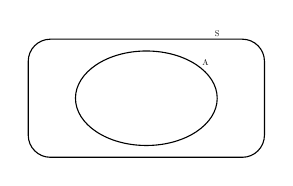
\begin{tikzpicture}
[scale=0.3]
\draw [,rounded corners=8pt, -] (0,-0) -- (0,5) -- (10,5) -- (10,0) -- cycle;
\draw (5,2.5) ellipse (3cm and 2cm);
\node [scale=0.3] at (7.5,4) {A};
\node [scale=0.3] at (8,5.25) {S};
\end{tikzpicture}\end{center}
Figura 9.10: Representação de conjuntos no diagrama de Venn
\end{quote}

Ao realizar um experimento aleatório, dizemos que um evento \(A\) ocorreu, se o resultado tiver sido um elemento de \(A\). Por exemplo, se ao lançarmos um dado com as faces numeradas de 1 a 6, tiver ocorrido face 2 e \(A\) é o evento “a face voltada para cima corresponde a um número par”, isto é, \(A=\{2,4,6\}\), dizemos que o evento \(A\) ocorreu.
\begin{quote}

\begin{figure}[H]
\centering

\noindent\sphinxincludegraphics[width=200\sphinxpxdimen]{{dados}.png}
\end{figure}

Figura 9.11: Dados comuns de seis faces numeradas de 1 a 6
\end{quote}
\begin{description}
\item[{Evento elementar: subconjunto unitário do espaço amostral \(S\); ou, equivalentemente, subconjunto do espaço amostral \(S\) no qual há apenas um resultado possível.\index{Evento elementar: subconjunto unitário do espaço amostral !ou, equivalentemente, subconjunto do espaço amostral  no qual há apenas um resultado possível.|textbf}}] \leavevmode\phantomsection\label{\detokenize{PE511-1:term-evento-elementar-subconjunto-unitario-do-espaco-amostral-ou-equivalentemente-subconjunto-do-espaco-amostral-no-qual-ha-apenas-um-resultado-possivel}}
\end{description}

Por exemplo, no lançamento de um dado, podemos representar o espaço amostral por \(S=\{1,2,3,4,5,6\}\). Nesse caso, os eventos elementares são os conjuntos unitários:
\begin{equation*}
\begin{split}\{1\}, \{2\}, \{3\}, \{4\}, \{5\} \textsf{ e } \{6\}.\end{split}
\end{equation*}
\sphinxstylestrong{Operações de união, interseção e complementariedade}

Faremos agora uma rápida revisão sobre operações entre conjuntos (união, interseção e complementariedade), pois eventos são conjuntos e nós estamos interessados em calcular probabilidades de eventos.
\begin{enumerate}
\item {} 
União: O conjunto \(A\cup B\) (lê-se \(A\)  união \(B\)) corresponde à reunião de todos os elementos de \(A\) e {}` de \(B\). Veja na figura 9.12, uma representação de \(A\cup B\), usando diagrama de Venn, em que o conjunto \(A\cup B\) corresponde à região pintada.
\phantomsection\label{\detokenize{PE511-1:fig-coloque-aqui-o-nome}}
\begin{figure}[H]
\centering

\noindent\sphinxincludegraphics[width=300bp]{{auniaoB1}.png}
\label{\detokenize{PE511-1:fig-coloque-aqui-o-nome}}\end{figure}

Figura 9.12: \(A\cup B\)

Dizemos que o evento \(A\cup B\) ocorreu se pelo menos um dos dois eventos, \(A\) ou \(B\), tiver ocorrido.

\item {} 
Interseção: O conjunto \(A\cap B\) (lê-se \(A\) interseção \(B\)) corresponde à coleção de todos os elementos que pertencem simultaneamente ao conjunto \(A\) e ao conjunto \(B\). Veja na figura 9.13 uma representação de \(A\cap B\), usando diagrama de Venn, em que o conjunto \(A\cap B\) corresponde à região pintada.
\begin{quote}
\begin{center}\begin{tikzpicture}
[scale=0.3]
\draw [,rounded corners=8pt, -] (0,-0) -- (0,5) -- (8,5) -- (8,0) -- cycle;
\node[scale=0.3] at (7,4) {B};
\node[scale=0.3] at (.5,4) {A};
\node[scale=0.3] at (7,5.25) {S};
\draw (5,2.5) circle (2cm);
\clip [draw] (2.5,2.5) circle (2cm);
\draw [fill= primario] (5,2.5) circle (2cm);
\end{tikzpicture}\end{center}\end{quote}

Figura 9.13: \(A\cap B\)

Dizemos que o evento \(A \cap B\) ocoreu, se os eventos \(A\) e \(B\) tiverem ocorrido simultaneamente.

\item {} 
Complementariedade: O conjunto \(\bar{A}\) (lê-se \(A\) complementar) corresponde à coleção de todos os elementos do conjunto universo (espaço amostral \(S\)) que não pertencem ao conjunto \(A\). Veja na figura 9.14 uma representação de \(\bar{A}\), usando diagrama de Venn, em que o conjunto \(\bar{A}\) corresponde à região pintada.
\begin{quote}
\begin{center}\begin{tikzpicture}
[scale=0.3]
\draw [,fill=primario!60,rounded corners=8pt, -] (0,-0) -- (0,5) -- (8,5) -- (8,0) -- cycle;
\node [scale=0.3] at (7,4) {$\overline{\rm A}$};
\node [scale=0.3] at (.5,4) {A};
\node [scale=0.3] at (7,5.25) {S};
\draw[fill=white] (2.5,2.5) circle (2cm);
\end{tikzpicture}\end{center}\end{quote}

Figura 9.14: Evento complementar de \(A: \bar{A}\)

Dizemos que o evento \(\bar{A}\) ocorreu, se o evento \(A\) não tiver ocorrido.

\end{enumerate}

Pela definição das operações de união, interseção e complementareidade dizemos que
\begin{enumerate}
\item {} 
o evento \(A\cup B\)  ocorreu se, e somente se, pelo menos um dos dois eventos \(A\) ou \(B\) tiverem ocorrido;

\item {} 
o evento \(A\cap B\) ocorreu se, e somente se, os dois eventos \(A\) e \(B\) tiverem ocorrido simultanemante.

\item {} 
o evento \(\bar{A}\) ocorreu se, e somente se, o evento \(A\) \sphinxstylestrong{não} tiver ocorrido.

\end{enumerate}
\begin{description}
\item[{Dois eventos \(A\)  e \(B\) são ditos (eventos) disjuntos se \(A\cap B=\emptyset\), ou seja, se \(A\) e \(B\) não tiverem elementos em comum.\index{Dois eventos   e  são ditos (eventos) disjuntos se , ou seja, se  e  não tiverem elementos em comum.|textbf}}] \leavevmode\phantomsection\label{\detokenize{PE511-1:term-dois-eventos-e-sao-ditos-eventos-disjuntos-se-ou-seja-se-e-nao-tiverem-elementos-em-comum}}
\end{description}

Dado qualquer espaço amostral \(S\), os conjuntos \(S\) e \(\emptyset\) (conjunto vazio) são considerados eventos especiais e chamados de \sphinxstylestrong{evento certo} e \sphinxstylestrong{evento impossível}, respectivamente.

Para o evento certo (\(S\)) atribui-se probabilidade 1 e, para o evento impossível (\(\emptyset\)), atribui-se probabilidade zero. Para qualquer outro evento, a probabilidade deverá ser um número real no intervalo {[}0,1{]}.

Para concluir essa breve revisão de operações com conjuntos, vamos apresentar a propriedade distributiva da operação de interseção com a união de dois eventos, a saber,
\begin{equation*}
\begin{split}(A\cup B)\cap C=(A\cap C)\cup (B\cap C)\end{split}
\end{equation*}
Para visualizar melhor essa propriedade, considere A, B e C eventos em um espaço amostral S, representados nos diagramas de Venn da figura 9.15, lembrando que as interseções nesses diagramas podem ser conjuntos vazios.
\begin{quote}
\begin{center}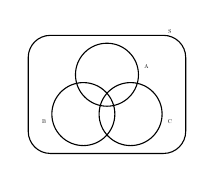
\begin{tikzpicture}
[scale=0.2]
\draw [,rounded corners=8pt,] (0,0) -- (0,7.5) -- (10,7.5) -- (10,0) -- cycle;
\node [scale=0.2] at (9,7.75) {S};
\draw (3.5,2.5) circle (2cm);
\node [scale=0.2] at (1,2) {B};
\draw (6.5,2.5) circle (2cm);
\node [scale=0.2] at (9,2) {C};
\draw (5,5) circle (2cm);
\node [scale=0.2] at (7.5,5.5) {A};
\end{tikzpicture}\end{center}\begin{center}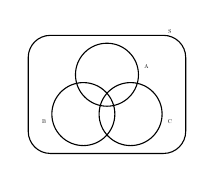
\begin{tikzpicture}
[scale=0.2]
\draw [,rounded corners=8pt,] (0,0) -- (0,7.5) -- (10,7.5) -- (10,0) -- cycle;
\node [scale=0.2] at (9,7.75) {S};
\draw (3.5,2.5) circle (2cm);
\node [scale=0.2] at (1,2) {B};
\draw (6.5,2.5) circle (2cm);
\node [scale=0.2] at (9,2) {C};
\draw (5,5) circle (2cm);
\node [scale=0.2] at (7.5,5.5) {A};
\end{tikzpicture}\end{center}
Figura 9.15: Diagramas de Venn com três conjuntos: \(A\), \(B\)  e \(C\)
\end{quote}

No primeiro diagrama, pinte de uma cor \(A\cup B\) e com outra cor, pinte o conjunto \(C\), destacando a região que foi pintada pelas duas cores. No segundo diagrama, pinte o conjunto \(A\cap C\) e, com a mesma cor,  o conjunto \(B\cap C\). A região pintadada corresponde ao conjunto dado no lado direito da igualdade. Finalmente, verifique que as regiões destacadas correspondem ao mesmo conjunto.

A seguir, serão apresentadas três interpretações da probabilidade.


\subsection{Interpretação clássica de probabilidade}
\label{\detokenize{PE511-1:interpretacao-classica-de-probabilidade}}
Na \index{interpretação clássica de probabilidade}interpretação clássica de probabilidade todos os eventos elementares são considerados igualmente prováveis (equiprováveis).

Esta interpretação costuma ser usada em problemas envolvendo lançamento de dados,  sorteios de cartas de um baralho e outros jogos. De fato, os primeiros trabalhos teóricos publicados envolvendo probabilidades no século XVII, fazem uso desta interpretação e envolvem cálculos de probabilidades de eventos em jogos de azar.

No entanto, nem sempre a interpretação clássica será adequada: lembre-se do exemplo da queda de um corpo celeste.

Um outro problema com esta interpretação é a circularidade do conceito de probabilidade para definir a própria probabilidade, pois considera em sua definição “resultados igualmente prováveis” que depende do conceito de probabilidade.


\subsection{Interpretação frequentista de probabilidade}
\label{\detokenize{PE511-1:interpretacao-frequentista-de-probabilidade}}
Na \index{interpretação frequentista de probabilidade}interpretação frequentista de probabilidade, a probabilidade de um evento é definida como a frequência relativa de ocorrência deste evento, se o experimento for repetido, sob as mesmas condições, um grande número de vezes.

Problemas com esta definição envolvem falta de clareza: o que siginificam
\begin{enumerate}
\item {} 
“sob as mesmas condições”? e

\item {} 
“um grande número de vezes”?

\end{enumerate}

Além disso, existem fenômenos únicos para os quais não é possível realizar repetições, por exemplo, o experimento que envolve verificar se daqui a 8 anos seu nível de instrução será superior completo ou não.

No entanto, esta interpretação é muito útil e amplamente usada em modelagens probabilísticas. De fato, a interpretação frequentista de probabilidade tem suas origens com a Lei dos Grandes Números, importante resultado da teoria das probabilidades estabelecido pelo matemático suíço Jakob Bernoulli (1654 - 1705). Bernoulli levou mais de vinte anos para provar a fórmula matemática, que foi publicada em seu livro “A Arte da Conjectura” (Ars Conjectandi) por seu sobrinho Nicolau Bernoulli em 1713. Bernoulli afirmou que quanto maior o número de tentativas (repetições do experimento), mais a proporção de tentativas bem-sucedidas (frequência relativa de ocorrência do evento de interesse) se aproxima de \(p\) (probabilidade do evento de interesse ocorrer).
\begin{quote}

\begin{figure}[H]
\centering

\noindent\sphinxincludegraphics[width=200\sphinxpxdimen]{{jakob_bernoulli}.png}
\end{figure}

Figura 9.16: Jakob Bernoulli (1654-1705)
\end{quote}

Veja na figura 9.17 uma ilustração da Lei dos Grandes Números na qual mostra-se uma \index{simulação}simulação do lançamento de uma moeda honesta (probabilidades iguais de cara e coroa) 1000 vezes. Os gráficos  ilustram a frequência relativa de caras, ou seja, número de caras obtidas sobre o número de lançamentos da moeda (eixo vertical) em função do número de lançamentos da moeda (eixo horizontal). A linha horizontal indica o valor \(\frac{1}{2}=0,5\), a probabilidade teórica de ocorrer cara para uma moeda honesta. Observe como rapidamente a frequência relativa se aproxima do valor \(\frac{1}{2}\).
\begin{quote}

\begin{figure}[H]
\centering

\noindent\sphinxincludegraphics[width=400\sphinxpxdimen]{{1000_lancamentos2}.png}
\end{figure}

Figura 9.17: Simulação do lançamento de uma moeda honesta 1000 vezes com destaque para  os 100 primeiros lançamentos da moeda.

\begin{figure}[H]
\centering

\noindent\sphinxincludegraphics[width=400\sphinxpxdimen]{{100_lancamentos2}.png}
\end{figure}

Figura 9.18: 100 primeiros lançamentos da moeda com destaque para os 10 primeiros lançamentos

\begin{figure}[H]
\centering

\noindent\sphinxincludegraphics[width=400\sphinxpxdimen]{{10_lancamentos2}.png}
\end{figure}

Figura 9.19: 10 primeiros lançamentos da moeda
\end{quote}

Observe que nesta simulação ocorreu cara no primeiro lançamento da moeda de tal modo que a frequência relativa de caras inicial é 1.  Além disso, nota-se que nas repetições iniciais a frequência relativa de caras oscila muito mais, no entanto, rapidamente ela se aproxima de 0,5 com uma oscilação desprezível.

Observando a figura 9.19, o que você diria que ocorreu (cara ou coroa), no terceiro lançamento da moeda? Por quê?

\begin{sphinxadmonition}{note}{Para o professor}

Sugere-se como atividade para ilustrar a lei dos grandes números dividir a turma em pelo menos 4 grupos e pedir a cada grupo que lance uma moeda fornecida pelo professor 10 vezes, registrando sequencialmente as caras e coroas obtidas. Após os lançamentos, ordene os grupos ao acaso e vá calculando as frequências relativas de caras, ilustrando-as em um gráfico cartesiano, como na figura 9.16.

Sugere-se disponibilizar as sequências de caras e coroas obtidas nos diferentes grupos e perguntar se a aparência do gráfico será muito diferente ao considerar outras ordenações dos grupos.

Referência: \sphinxurl{https://www.ime.usp.br/~abe/ce-arquivos/Oficina.pdf}
\end{sphinxadmonition}


\subsection{Interpretação subjetiva de probabilidade}
\label{\detokenize{PE511-1:interpretacao-subjetiva-de-probabilidade}}
Na \index{interpretação subjetiva de probabilidade}interpretação subjetiva de probabilidade, probabilidades de eventos são designadas de acordo com a experiência que o pesquisador tem sobre o fenômeno em investigação. No primeiro exemplo desta seção (queda de um corpo celeste) pode-se dizer que adotou-se a interpretação subjetiva quando atribui-se uma probabilidade pequena, próxima de zero, para o evento “não cair”.

Uma crítica a esta interpretação é a de que pessoas diferentes podem atribuir probabilidades diferentes para um mesmo evento. No entanto, observe que as outras duas interpretações também são subjetivas.

O importante, quando adota-se a interpretação subjetiva, é ter coerência. Por exemplo se sabemos que um evento \(A\) ocorre com frequência quatro vezes maior do que um evento \(B\), então \(P(A)=4\cdot P(B)\).

Se temos a percepção de que é mais provável que certo evento ocorra do que ele não ocorra, atribuímos a ele uma probabilidade maior do que 0,5. Por outro lado, se temos a percepção de que é menos provável que certo evento ocorra do que ele não ocorra, atribuímos a ele uma probabilidade inferior a 0,5. Se temos a percepção de que não existe favorecimento entre a ocorrência ou não de certo evento, ou mesmo se não sabemos nada sobre ele, atribuímos a ele uma probabilidade de 0,5. A razão pela qual usamos o valor 0,5 como referência se dá pelo fato de que 0,5 é exatamente o centro da escala da probabilidade que varia de 0 a 1 (0 a 100\%) como será formalizado na Seção {\hyperref[\detokenize{PE511-4:sec-organizando-propriedades}]{\sphinxcrossref{\DUrole{std,std-ref}{Organizando: Probabilidade - regras básicas e propriedades}}}}.


\practice{ Probabilidade \textendash{} conceitos básicos}
\label{\detokenize{PE511-2:praticando-probabilidade-conceitos-basicos}}\label{\detokenize{PE511-2::doc}}\begin{sphinxadmonition}{note}{Atividade}{espaço amostral não é único!}
\label{ativ-espaco-amostral-nao-e}

\begin{sphinxadmonition}{note}{Para o professor}

\sphinxstylestrong{Objetivos específicos}  Reconhecer a não unicidade do espaço amostral.

\sphinxstylestrong{Observações e sugestões} Nesta atividade pretende-se discutir com o aluno a não unicidade do espaço amostral. Esta discussão é importante, pois dependendo da forma como o espaço amostral é especificado, pode-se ter eventos elementares que são equiprováveis ou não. Além disso, algumas representações do espaço amostral de um experimento poderão responder a mais perguntas do que outras. Por exemplo, no primeiro item, a discriminação de todas as sequências possíveis de ordem de nascimentos permite  responder perguntas sobre o sexo do filho mais velho, etc. Já no segundo item, perguntas deste tipo nem sempre podem ser respondidas.

\begin{sphinxadmonition}{note}{Resposta}

\begin{enumerate}
\item {} 
Usando \(\textsf{a}\) para menina e \(\textsf{o}\) para menino, pode-se identificar todas as possibilidades, construindo-se o seguinte diagrama, chamado diagrama de árvore.

\end{enumerate}
\begin{center}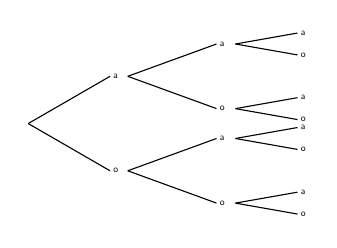
\begin{tikzpicture}
[scale=0.4]
\draw (0,0) -- (30:3) node [right, scale=0.35] {$\textsf{a}$};
\draw (0,0) -- (-30:3) node [right, scale=0.35] {$\textsf{o}$};
\draw (3.159807,1.5) -- ++(20:3) node [right, scale=0.35] {$\textsf{a}$};
\draw (3.159807,1.5) -- ++(-20:3) node [right, scale=0.35] {$\textsf{o}$};
\draw (3.159807,-1.5) -- ++(20:3) node [right, scale=0.35] {$\textsf{a}$};
\draw (3.159807,-1.5) -- ++(-20:3) node [right, scale=0.35] {$\textsf{o}$};
\draw  (6.57888,2.5260) -- ++(10:2) node [right, scale=0.35] {$\textsf{a}$};
\draw  (6.57888,2.5260) -- ++(-10:2) node [right, scale=0.35] {$\textsf{o}$};
\draw  (6.57888,0.4739) -- ++(10:2) node [right, scale=0.35]   {$\textsf{a}$};
\draw  (6.57888,0.4739) -- ++(-10:2) node [right, scale=0.35]   {$\textsf{o}$};
\draw  (6.57888,-0.4739) -- ++(10:2) node [right, scale=0.35]  {$\textsf{a}$};
\draw  (6.57888,-0.4739) -- ++(-10:2) node [right, scale=0.35] {$\textsf{o}$};
\draw  (6.57888,-2.5260) -- ++(10:2) node [right, scale=0.35]   {$\textsf{a}$};
\draw  (6.57888,-2.5260) -- ++(-10:2) node [right, scale=0.35] {$\textsf{o}$};
\end{tikzpicture}\end{center}
Diagrama de árvore: representação das oito possibilidades de nascimentos de três filhos

\(S=\{\textsf{ (a,a,a),(a,a,o), (a,o,a),(a,o,o),(o,a,a),(o,a,o),(o,o,a),(o,o,o)}\}\)
com, por exemplo, \(\textsf{(a,o,a)}\) indicando que dos três filhos, o primeiro foi uma menina, o segundo foi um menino e, o terceiro, uma menina. Observe que neste caso, \(\#(S)=8\) e, se as probabilidades de nascer um menino e de nascer uma menina são iguais, é natural usar a interpretação clássica de probabilidade, atribuindo probabilidades iguais a cada um dos 8 eventos elementares deste espaço amostral. Lembre que eventos elementares são os subconjuntos unitários do espaço amostral.
\begin{enumerate}
\item {} 
Se formos pensar na quantidade de meninas do casal tem-se \(S=\{0,1,2,3\}\). Observe que neste caso \(\#(S)=4\), mas neste caso não será adequado atribuir probabilidades iguais aos eventos elmentares \(\{0\}\), \(\{1\}\),  \(\{2\}\) e \(\{3\}\), pois claramente, os eventos \(\{1\}\) e \(\{2\}\) ocorrem com maior frequência e, portanto, com maior probabilidade. Veja as oito situações possíveis no item anterior e quantas delas correspondem a estes dois eventos elementares.

\end{enumerate}
\end{sphinxadmonition}
\end{sphinxadmonition}

Considere as famílias com três filhos no bairro onde você mora. Suponha que deseja-se calcular probabilidades do tipo: “qual a probabilidade de que uma dessas famílias com três filhos tenha dois meninos e uma menina?”.
\begin{enumerate}
\item {} 
Construa um espaço amostral adequado para calcular esta probabilidade, considerando as possíveis sequências de nascimentos dos três filhos na família.

\item {} 
Construa um outro espaço amostral, considerando a quantidade de meninas em cada casal de três filhos.

\end{enumerate}
\end{sphinxadmonition}
\begin{sphinxadmonition}{note}{Atividade}{avaliando probabilidades a partir de um histograma}
\label{ativ-probabilidade-histograma}

\begin{sphinxadmonition}{note}{Para o professor}

\sphinxstylestrong{Objetivos específicos}  Avaliar probabilidades de eventos usando dados quantitativos coletados, representados em um histograma e em uma tabela de frequências.

\sphinxstylestrong{Observações e sugestões}  A partir de dados coletados e representados por meio de um histograma, os alunos deverão responder perguntas referentes a probabilidades de certos eventos e para isso deverão usar a noção frequentista de probabilidade.

\begin{sphinxadmonition}{note}{Resposta}

Para responder as questões desta atividade será usada a interpretação frequentista de probabilidade.
\begin{enumerate}
\item {} 
Pela tabela de frequências observa-se que 19 tempos de chegada dos 100 melhores estão no intervalo dado, portanto, a probabilidade será \(\frac{19}{100}=0,19\).

\item {} 
Pela tabela de frequências observa-se que há \(100-24-19=57\) tempos de chegada entre os 100 melhores que são inferiores a 154,0 minutos. Portanto a probabilidade será \(\frac{57}{100}=0,57\). A resposta poderia ser obtida também, somando-se as frequências dos intervalos de classe do início até o intervalo {[}151,0 ; 154,0{[}: \(7+4+1+2+4+4+14+21=57\), obtendo-se 0,57 como probabilidade.

\item {} 
Pela tabela, vemos que 152,5 minutos não é extremo de intervalo na construção apresentada, desse modo podemos concluir que a probabilidade solicitada será um número no intervalo {]}0,43 ; 0,64{[}. Observe que 152,5 está no intervalo {[}151,0 ; 154,0{[} de comprimento 3, cuja frequência absoluta é 21. Observe também que o subintervalo {[}152,5; 154,0{[}  de {[}151,0 ; 154,0{[} tem comprimento 1,5. Usando a suposição de proporcionalidade da frequência em cada intervalo por unidade de comprimento do intervalo, podemos a aproximar a frequência do subintervalo por \(21\times \frac{1,5}{3}=10,5\). Logo, a probabilidade será obtida por \(\frac{10,5+24+19}{100}=\frac{53,5}{100}=0,535\) que de fato é um número no intervalo inicialmente obtido.

\item {} 
Pela tabela, nem 152,5 nem 158,0 são extremos de intervalo, porém podemos obter um limite  superior para a probabilidade solicitada, que neste caso será um número menor do que 0,64 (\((21+24+19)/100\)).  Para um valor pontual, serão necessárias duas aproximações de frequências. A primeira no intervalo {[}152,5; 154,0{[} já realizada no item anterior que foi aproximada para 10,5. A frequência do intervalo {[}154,0 ; 157,0 {[} é 24. Para o intervalo {[}157,0 ; 158,0{[} calcularemos uma frequência aproximada, usando o argumento da proporcionalidade. O intervalo {[}157,0 ; 160,0{[} tem comprimento 3 com frequência 10, então, uma aproximação para o subintervalo {[}157,0 ; 158,0{[} de {[}157,0 ; 160,0{[} de comprimento 1 é dada por \(19\times \frac{1}{3}\approx 6,3\). Assim, a probabilidade será \(\frac{10,5+24+6,3}{100}=\frac{40,8}{100}=0,408\).

\end{enumerate}
\end{sphinxadmonition}
\end{sphinxadmonition}
\end{sphinxadmonition}

No capítulo Medidas de posição e dispersão foram trabalhados os dados sobre os 100 melhores tempos atingidos na Maratona de Nova Iorque (2017) para as categorias homens e mulheres. Na figura 9.19, apresenta-se um histograma construído para os 100 melhores tempos na maratona de Nova Iorque (2017) para a categoria homens, após a conversão destes tempos para minutos.
\begin{quote}

\begin{figure}[H]
\centering

\noindent\sphinxincludegraphics[width=600bp]{{histogrsms_homens_b_1}.png}
\end{figure}

Figura 9.20: Histograma dos 100 melhores tempos para homens na Maratona de Nova Iorque (2017), destacando a frequ\textasciitilde{}encia absoluta de cada intervalo de classe.
\end{quote}

Na tabela 9.1 são apresentados os intervalos de classe e suas respectivas frequências, usados na construção do histograma da figura 9.20. Os intervalos considerados são fechados à esquerda e abertos à direita.
\begin{quote}

Tabela 9.1: Distribuição de frequências dos 100 melhores tempos na categoria homens da maratona de Nova Iorque (2017)


\begin{savenotes}\sphinxattablestart
\centering
\begin{tabular}[t]{|*{3}{\X{1}{3}|}}
\hline

Intervalo de classe
&\begin{description}
\item[{Frequência}] \leavevmode
absoluta

\end{description}
&\begin{description}
\item[{Frequência}] \leavevmode
relativa

\end{description}
\\
\hline
{[} 130,0 ; 133,0  {[}
&
7
&
0,07
\\
\hline
{[} 133,0 ; 136,0 {[}
&
4
&
0,04
\\
\hline
{[} 136,0 ; 139,0 {[}
&
1
&
0,01
\\
\hline
{[} 139,0 ; 142,0 {[}
&
2
&
0,02
\\
\hline
{[}142,0 ; 145,0 {[}
&
4
&
0,04
\\
\hline
{[} 145,0 ; 148,0 {[}
&
4
&
0,04
\\
\hline
{[} 148,0 ; 151,0 {[}
&
14
&
0,14
\\
\hline
{[} 151,0 ; 154,0 {[}
&
21
&
0,21
\\
\hline
{[} 154,0 ; 157,0 {[}
&
24
&
0,24
\\
\hline
{[} 157,0 ; 160,0 {[}
&
19
&
0,19
\\
\hline
\end{tabular}
\par
\sphinxattableend\end{savenotes}
\end{quote}

Suponha que o comportamento dos 100 melhores tempos para homens na Maratona de Nova Iorque (2017) represente bem os 100 melhores tempos para homens em qualquer Maratona de Nova Iorque

Com base nessa suposição, estime a probabilidade de que na próxima maratona de Nova Iorque o tempo de conclusão da corrida, entre os 100 melhores na categoria homens,
\begin{enumerate}
\item {} 
ocorra entre 157,0 e 160,0 minutos;

\item {} 
seja inferior a 154,0 minutos;

\item {} 
seja superior a 152,5 minutos;

\item {} 
caia entre 152,5 e 158 minutos.

Observação: Para responder os dois últimos itens, suponha, em cada intervalo, que as frequências obervadas são proporcionais aos comprimentos dos intervalos, para poder avaliar frequências em subintervalos.

\end{enumerate}
\begin{sphinxadmonition}{note}{Atividade}{Leis de De Morgan}
\label{ativ-leis-de-demorgan}

\begin{sphinxadmonition}{note}{Para o professor}

\sphinxstylestrong{Objetivos específicos}  Reconhecer propriedades importantes de operações com conjuntos, envolvendo união, interseção e complementação.
\begin{quote}

\begin{sphinxadmonition}{note}{Resposta}

\begin{enumerate}
\item {} 
Veja a figura a seguir. No primeiro diagrama foi pintada a região correspondente ao complementar da interseção de \(A\) e \(B\). No segundo diagrama foi realçada em listras vermelhas a região que corresponde ao evento \(\bar{A}\) e em listras azuis a região que corresponde ao evento \(\bar{B}\). Depois, em cinza foi destacada a região correspondendo à união dos dois. Verifique que correspondem à mesma região.

\end{enumerate}
\end{sphinxadmonition}
\phantomsection\label{\detokenize{PE511-2:fig-coloque-aqui-o-nome}}
\begin{figure}[H]
\centering

\noindent\sphinxincludegraphics[width=200bp]{{demorgan1}.png}
\label{\detokenize{PE511-2:fig-coloque-aqui-o-nome}}\end{figure}

\begin{figure}[H]
\centering
\capstart

\noindent\sphinxincludegraphics[width=200bp]{{demorgan2}.png}
\caption{As leis de De Morgan podem ser enunciadas da seguinte forma:}
\begin{sphinxlegend}\begin{enumerate}
\item {} 
O complementar da interseção de dois eventos é igual a união dos complementares desses dois eventos.

\item {} 
O complementar da união de dois eventos é igual a interseção dos complementares desses dois eventos.

\end{enumerate}
\end{sphinxlegend}
\label{\detokenize{PE511-2:id1}}\label{\detokenize{PE511-2:id3}}\end{figure}
\end{quote}
\end{sphinxadmonition}

Verifique, usando diagrama de Venn, as seguintes igualdades, conhecidas como as Leis de De Morgan. Sejam \(A\) e \(B\) dois conjuntos, então
\begin{enumerate}
\item {} 
\(\displaystyle{\overline{A\cap B}}=\bar{A}\cup \bar{B}\)

\item {} 
\(\overline{A\cup B}=\bar{A}\cap \bar{B}\)

\end{enumerate}
\end{sphinxadmonition}
\begin{sphinxadmonition}{note}{Atividade}{Distributividade}
\label{ativ-distributividade}

\begin{sphinxadmonition}{note}{Para o professor}

\sphinxstylestrong{Objetivo específico:} Verificar a propriedade distribuitiva da operação de interseção de conjuntos com a operação de união de conjuntos.

\sphinxstylestrong{Observações e sugestões:} Dois diagramas de venn são apresentados. A ideia é realizar a verificação pintando os diagramas conforme a operação à esquerda e à direita da igualdade, para concluir que se referem ao mesmo conjunto.
\begin{quote}

\begin{sphinxadmonition}{note}{Resposta}
\begin{quote}
\phantomsection\label{\detokenize{PE511-2:id2}}
\begin{figure}[H]
\centering

\noindent\sphinxincludegraphics[width=300bp]{{distributividade}.png}
\label{\detokenize{PE511-2:id2}}\end{figure}
\end{quote}

Figura: Diagramas de Venn: \((A\cap B)\cup C=(A\cup C)\cap (B\cup C)\)

No diagrama da esquerda tem-se em amarelo a região indicada pela expressão à esquerda na igualdade a ser verificada. No diagrama da direita tem-se \(A\cup C\) em listras vermelhas, \(B\cup C\) em listras azuis. A região da interseção dos dois é a que contêm listras azuis e vermelhas e está destacada na cor cinza. Observe que é a mesma região em amarelo do diagrama da esquerda.
\end{sphinxadmonition}
\end{quote}
\end{sphinxadmonition}
\end{sphinxadmonition}

Verifique, usando os diagramas de Venn na figura 9.20, a propriedade distributiva da operação de união com a interseção de dois conjuntos.
\begin{quote}
\begin{equation*}
\begin{split}(A\cap B)\cup C=(A\cup C)\cap (B\cup C)\end{split}
\end{equation*}\begin{center}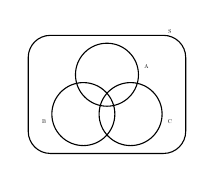
\begin{tikzpicture}
[scale=0.2]
\draw [,rounded corners=8pt,] (0,0) -- (0,7.5) -- (10,7.5) -- (10,0) -- cycle;
\node [scale=0.2] at (9,7.75) {S};
\draw (3.5,2.5) circle (2cm);
\node [scale=0.2] at (1,2) {B};
\draw (6.5,2.5) circle (2cm);
\node [scale=0.2] at (9,2) {C};
\draw (5,5) circle (2cm);
\node [scale=0.2] at (7.5,5.5) {A};
\end{tikzpicture}\end{center}\begin{center}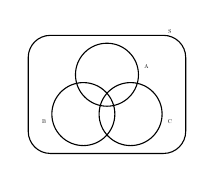
\begin{tikzpicture}
[scale=0.2]
\draw [,rounded corners=8pt,] (0,0) -- (0,7.5) -- (10,7.5) -- (10,0) -- cycle;
\node [scale=0.2] at (9,7.75) {S};
\draw (3.5,2.5) circle (2cm);
\node [scale=0.2] at (1,2) {B};
\draw (6.5,2.5) circle (2cm);
\node [scale=0.2] at (9,2) {C};
\draw (5,5) circle (2cm);
\node [scale=0.2] at (7.5,5.5) {A};
\end{tikzpicture}\end{center}
Figura 9.20: Diagramas de Venn com três conjuntos: \(A\), \(B\)  e \(C\)
\end{quote}
\begin{quote}

\begin{sphinxadmonition}{note}{Para o professor}
\begin{quote}

Esta seção da unidade temática de Probabilidade tem como objetivo principal apresentar uma definição matemática de probabilidade, independente das interpretações apresentadas na seção 1, conhecida como definição axiomática da probabilidade. Os axiomas dessa definição serão, no livro, chamados de regras básicas da probabilidade, a saber,
\end{quote}
\begin{enumerate}
\item {} 
a probabilidade de um evento é um número não-negativo,

\item {} 
a probabilidade do evento certo (espaço amostral) é 1 (Dizemos que um evento ocorreu, se o resultado observado for um dos elementos do evento. Observe que sempre ocorrerá um elemento do espaço amostral que contém todos os resultados possíveis, por essa razão, ele costuma ser chamado de evento certo. Lembre-se que todo conjunto é subconjunto de si próprio e, portanto, o espaço amostral pode ser considerado como um evento, assim como o conjunto vazio.),

\item {} 
dados dois eventos disjuntos A e B (\(A\cap B=\emptyset\)), a probabilidade da união dos dois é dada pela soma das probabilidades P(A)+P(B). De fato, na definição formal de medida de probabilidade, este terceiro axioma deve incluir uma coleção enumerável de eventos dois a dois disjuntos tal que a probabilidade da união enumerável desses eventos é dada pela soma enumerável das probabilidades de cada um deles. Este axioma é chamado axioma da sigma-aditividade da probabilidade. No entanto, entendemos que nesse nível de ensino, não será necessário apresentar a definição axiomática completa. Este último axioma, será estendido para uniões disjuntas (uniões de eventos disjuntos) de um número finito de eventos disjuntos dois a dois.

\end{enumerate}

A introdução da definição axiomática da probabilidade, a mesma será considerada sob cada uma das interpretações trabalhadas na seção inicial da unidade, de modo que na interpretação clássica, obteremos a probabilidade de um evento como a razão do número de elementos do evento sobre número de elementos do espaço amostral; na interpretação frequentista, obteremos a probabilidade de um evento como a frequência relativa de ocorrência desse evento quando repetimos o experimento um grande número de vezes sob as mesmas condições e na interpretação subjetiva destacaremos a importância de sermos coerentes com os axiomas, no sentido de não atribuir probabilidades maiores que 1 ou negativas, lembrando também do axioma 3. O mais importante nessa discussão é perceber que em qualquer uma delas valerão os três axiomas.

Em seguida trabalharemos com propriedades derivadas dos axiomas, a saber, (1) a probabilidade do evento vazio (P(∅)=0), (2) a probabilidade do evento complementar (P(Ā)=1-P(A)), (3) se A⊂B, então P(A)≤P(B) e (4) a probabilidade da união de dois eventos quaisquer (P(A∪B)=P(A)+P(B)-P(A∩B)).

Nesta seção, será introduzida, embora de forma superficial, a questão da modelagem probabilística de um fenômeno, a partir de levantamento de dados. O intuito é mostrar como podemos usar dados de pesquisas para avaliar probabilidades. Basicamente, uma distribuição de frequências será usada para calcular probabilidades. Reforça-se a importância de, em tais situações, sempre destacar a suposição de que os dados observados refletem bem o comportamento da população cujas probabilidades ou estimativas serão calculadas a partir dos dados observados.

A seção é encerrada trabalhando-se com a noção de probabilidade geométrica para espaços amostrais contínuos. Nesse caso específico é importante frisar que estamos considerando como espaços amostrais contínuos conjuntos infinitos não-enumeráveis para os quais estão definidas medidas de comprimento ou área ou volume. Além disso, também estamos considerando que o modelo uniforme de probabilidade (função de densidade de probabilidade constante) é adequado para esses espaços. É claro que para o aluno, bastará mencionar que um ponto desse espaço será escolhido ao acaso de modo que subconjuntos de igual comprimento ou área ou volume do espaço amostral são equiprováveis. Nesses casos, dependendo da dimensão do espaço amostral (1, 2 ou 3), probabilidades serão calculadas como razão de comprimentos ou áreas ou volumes, respectivamente, observando-se a validade das regras básicas da probabilidade apresentadas no início da seção. É importante explorar nesse contexto as situações de eventos com infinitos elementos, mas cuja probabilidade é zero. Por exemplo, se o espaço amostral é um círculo de raio R, a probabilidade de sortearmos um ponto de um diâmetro fixado será zero, pois a medida da área definida pelo diâmetro é nula.

São objetivos específicos da seção 2:
\begin{enumerate}
\item {} 
OE6 {[}definição axiomática{]} - Aplicar as regras básicas da probabilidade nas diferentes interpretações de probabilidade.

\item {} 
OE7 {[}definição axiomática{]} - Aplicar as regras básicas da probabilidade para obter as regras da probabilidade do evento complementar e a probabilidade da união de dois eventos (propriedades da probabilidade).

\item {} 
OE8 {[}modelagem probabilística{]} - Avaliar, ainda que de forma incipiente, modelos para fenômenos aleatórios.

\item {} 
OE9 {[}aplicação{]} - Aplicar as regras básicas da probabilidade em espaços amostrais contínuos (probabilidade geométrica).

\end{enumerate}
\end{sphinxadmonition}
\end{quote}


\explore{ Probabilidade - regras básicas e propriedades}
\label{\detokenize{PE511-3:explorando-probabilidade-regras-basicas-e-propriedades}}\label{\detokenize{PE511-3:sec-regras-basicas}}\label{\detokenize{PE511-3::doc}}
No início do século XX, o matemático russo Kolmogorov, como já comentado na Seção {\hyperref[\detokenize{PE511-0:sec-conceitos-basicos}]{\sphinxcrossref{\DUrole{std,std-ref}{Explorando: Probabilidade \textendash{} conceitos básicos}}}}, estabeleceu regras básicas para a probabilidade que independem da interpretação adotada, possibilitando assim, a construção de uma teoria matemática de probabilidade.

De maneira simplificada, essas regras básicas serão apresentadas a seguir.

Seja \(S\) um espaço amostral. Uma probabilidade é uma função \(P\) que associa a cada subconjunto de \(S\) (evento)  um número real, tal que
\begin{enumerate}
\item {} 
ela é sempre um número não negativo,

\item {} 
a probabilidade do evento certo é igual a 1 e,

\item {} 
dados dois eventos disjuntos, a probabilidade da união dos dois é dada pela soma das probabilidades individuais.

\end{enumerate}

Em símbolos, essas regras podem ser apresentadas da seguinte forma:
\begin{enumerate}
\item {} 
\(P(A)\geq 0\) qualquer que seja \(A\subset S\), ou seja, a probabilidade de qualquer evento \(A\) é um número não-negativo.

\item {} 
\(P(S)=1\), ou seja, a probabilidade do evento certo é igual a 1.

\item {} 
Se \(A,B\subset S\) com \(A\) e \(B\) eventos disjuntos (\(A\cap B=\emptyset\)), então \(P(A\cup B)=P(A)+P(B)\).

\end{enumerate}
\begin{sphinxadmonition}{note}{Atividade}{censo Educação Física}
\label{ativ-probabilidade-atividade-fisica}

\begin{sphinxadmonition}{note}{Para o professor}

\sphinxstylestrong{Objetivos específicos}
\begin{enumerate}
\item {} 
Aplicar as regras básicas da probabilidade, usando a interpretação frequentista de probabilidade.

\item {} 
Aplicar as regras básicas da probabilidade para obter as regras da probabilidade do evento complementar e da probabilidade da união de dois eventos quaisquer.

\end{enumerate}

\begin{sphinxadmonition}{note}{Resposta}

\begin{enumerate}
\item {} 
\(P(A)=\frac{270}{800}=0,3375\), \(P(B)=\frac{240}{800}=0,3\), \(P(C)=\frac{150}{800}=0,1875\) e \(P(D)=\frac{140}{800}=0,175\).

\item {} 
De fato, \(S=A\cup B\cup C\cup D\) com \(A, B\), \(C\) e \(D\) dois a dois disjuntos. \(1=P(S)=P(A\cup B\cup C\cup D)=P(A)+P(B)+P(C)+P(D)=0,3375+0,3+0,1875+0,175=1\), o que era de se esperar em função das regras básicas da probabilidade.

\item {} 
Observe que podemos usar a interpretação clássica de probabilidade, considerando cada aluno da escola igualmente provável de ser escolhido. Como queremos a probabilidade de que o aluno pratique algum tipo de atividade física regular fora do período escolar, devemos contar quantos são estes alunos.  Uma maneira mais simples de contar estes alunos é calcular a diferença entre o total de alunos (800) e o número de alunos que \sphinxstylestrong{não} praticam atividade física (270), obtendo-se 530. Logo, a probabilidade solicitada é dada por \(\frac{530}{800}=0,6625\). É claro que também poderíamos somar os números de alunos que praticam cada um dos tipos de atividade física: \(240+150+140=530\). Mas, observe que a contagem obtida pelo cálculo da diferença entre o total e o número de alunos que não praticam atividade física foi mais simples: \(800-270=530\).

\item {} 
Sejam os eventos \(B\): “jogar futebol” e \(M:\) “ser do turno da manhã”. Observe que \(B\cap M\subset B\) tal que o número de elementos da interseção é menor ou igual ao número de elementos de \(B\) de modo que o evento \(B\) parece ser mais provável do que o evento \(B\cap M\). Olhando os dados, temos que a probabilidade de que o aluno jogue futebol é dada por \(P(B)=\frac{240}{800}=0,3\) e a probabilidade de jogar futebol \sphinxstylestrong{e} ser do turno da manhã é \(P(B\cap M)=\frac{160}{800}=0,2\). Logo, é mais provável escolher um aluno que jogue futebol do que escolher um aluno do turna da manhã que jogue futebol. Essa é uma propriedade importante da probabilidade: se \(A\subset B\), então \(P(A)\leq P(B)\).

\item {} 
Chamando de \(E\) o evento “praticar outra atividade diferente de futebol” e \(T\) o evento “ser do turno da tarde”, queremos calcular \(P(E\cup T)\).  Da tabela de dados temos que o total de alunos que praticam outra atividade diferente de futebol é \(150+140=290\) e o total dos alunos do turno da tarde é 350. No entanto, a soma \(290+350=640\) é superior ao número de alunos que tem pelo menos uma dessas duas características. Isso ocorre pois nos dois totais considerados, estamos contando os alunos que têm simultaneamente as duas características. Logo, devemos subtrair de 640 o valor \(70+70=140\) que representa o total de alunos que pratica outra atividade e é ao mesmo tempo do turno da tarde. Portanto, podemos escrever que

\end{enumerate}

\(P(E\cup T)=P(E)+P(T)-P(E\cap T)=\frac{290}{800}+\frac{350}{800}-\frac{140}{800}=\frac{500}{800}=0,625\).
\end{sphinxadmonition}
\end{sphinxadmonition}

Em uma escola de Ensino Médio há dois turnos: manhã e tarde. No turno da manhã há 450 alunos e, no turno da tarde, 350 alunos. Os professores de Educação Física realizaram um censo para saber se os alunos da escola praticavam algum tipo de atividade física regular fora do período escolar. A pergunta principal do questionário da pesquisa foi:

\sphinxstylestrong{Qual é a sua atividade física principal fora do período escolar? Marque apenas uma opção.}

\sphinxstylestrong{(  ) Não pratica  (   ) Futebol (  ) Outra}

Na tabela 9.2 estão os resultados obtidos.
\begin{quote}

Tabela 9.2: Distribuição de frequências por atividade, segundo o turno.
\end{quote}


\begin{savenotes}\sphinxattablestart
\centering
\begin{tabulary}{\linewidth}[t]{|T|T|T|T|}
\hline

Atividade Física
&
Manhã
&
Tarde
&
Total
\\
\hline
Não pratica
&
140
&
130
&
270
\\
\hline
Futebol
&
160
&
80
&
240
\\
\hline
Natação
&
80
&
70
&
150
\\
\hline
Outra atividade
&
70
&
70
&
140
\\
\hline
Total
&
450
&
350
&
800
\\
\hline
\end{tabulary}
\par
\sphinxattableend\end{savenotes}

Um aluno desta escola será escolhido ao acaso.
\begin{enumerate}
\item {} 
Considere os eventos \(A\):  ” o aluno escolhido não pratica atividade física”, \(B\): ” o aluno escolhido pratica Futebol como atividade física principal”, \(C\): ” o aluno escolhido pratica natação” e \(D:\): “o aluno pratica outro tipo de atividade física principal”. Determine a probabilidade de cada um desses eventos.

\item {} 
Observe que o espaço amostral nesse experimento corresponde à união dos eventos considerados no item anterior. Calcule a soma das probabilidades determinadas no item anterior. O resultado obtido é compatível com a segunda regra básica, a saber, \(P(S)=1\)? Por quê?

\item {} 
Qual é a probabilidade de que este aluno pratique algum tipo de atividade física regular fora do período escolar?

\item {} 
O que é mais provável: que o aluno escolhido seja do turno da manhã e jogue futebol ou que o aluno jogue futebol?

\item {} 
Qual é a probabilidade de que o aluno escolhido seja do turno da tarde \sphinxstylestrong{ou} pratique atividade física diferente de futebol, isto é, que o aluno escolhido tenha pelos menos uma dessas duas características?

\end{enumerate}
\end{sphinxadmonition}


\arrange{ Probabilidade - regras básicas e propriedades}
\label{\detokenize{PE511-4:sec-organizando-propriedades}}\label{\detokenize{PE511-4::doc}}\label{\detokenize{PE511-4:organizando-probabilidade-regras-basicas-e-propriedades}}
A última regra básica é chamada propriedade aditiva da probabilidade para eventos disjuntos e, de fato, é um caso particular da propriedade de aditividade da probabilidade.

Suponha três eventos \(A\), \(B\) e \(C\) disjuntos 2 a 2, ou seja, \(A\cap B=A\cap C=B\cap C=\emptyset\). A regra da aditividade para a união destes três eventos resultará em \(P(A\cup B\cup C)=P(A)+P(B)+P(C)\).
\begin{quote}
\begin{center}\begin{tikzpicture}
[scale=0.3]
\draw [,rounded corners=8pt, -] (0,0) -- (0,8) -- (10,8) -- (10,0) -- cycle;
\node [scale=0.3] at (9,8.25) {S};
\draw [fill=primario!60](2.5,2.2) circle (2cm);
\node [scale=0.3] at (.75,.5) {B};
\draw [fill=primario!60](7.5,2.2) circle (2cm);
\node [scale=0.3] at (9.25,.5) {C};
\draw [fill=primario!60](5,5.75) circle (2cm);
\node [scale=0.3] at (7.5,5.5) {A};
\end{tikzpicture}\end{center}
Figura 9.21: Três eventos A, B e C disjuntos dois a dois ilustrados no diagrama de Venn
\end{quote}

A propriedade de aditividade da probabilidade para eventos disjuntos vale para qualquer coleção de eventos disjuntos 2 a 2.


\subsection{Interpretações da probabilidade e as regras básicas}
\label{\detokenize{PE511-4:interpretacoes-da-probabilidade-e-as-regras-basicas}}
Como determinar probabilidades sob cada uma das interpretações apresentadas na Seção {\hyperref[\detokenize{PE511-1:sec-interpretacoes}]{\sphinxcrossref{\DUrole{std,std-ref}{Organizando as ideias: Probabilidade \textendash{} conceitos básicos}}}}, considerando as regras básicas?

\sphinxstylestrong{1. Interpretação clássica}

\begin{sphinxadmonition}{note}{Exemplo}

Considere o lançamento de um dado honesto (todas as faces ocorrem com probabilidades iguais). Neste caso o espaço amostral é dado por

\(S=\{ 1,2,3,4,5,6\}\) e, os eventos elementares, são dados por

\(A_1=\{1\}\), \(A_2=\{2\}\), \(A_3=\{3\}\), \(A_4=\{4\}\), \(A_5=\{5\}\) e \(A_6=\{6\}\).

Faça \(P(A_i)=k\), \(i=1,2,3,4,5,6\).

Observe que \(S=A_1\cup A_2\cup A_3\cup A_4\cup A_5 \cup A_6\) e que os eventos \(A_1\), \(A_2\), \(A_3\), \(A_4\) , \(A_5\) e \(A_6\) são disjuntos.

Usando as regras básicas, tem-se

\(1=P(S)=P(A_1\cup A_2\cup A_3\cup A_4\cup A_5 \cup A_6)=P(A_1)+P(A_2)+\cdots +P(A_6)=6\cdot k\)

Logo, \(k=\frac{1}{6}\).
\end{sphinxadmonition}

De modo mais geral, sob a interpretação clássica na qual o espaço amostral \(S\) é finito e todos os eventos elementares são equiprováveis, se o número de elementos do conjunto \(S\) é \(n\), \(n\in \mathbb{N}\), então a probabilidade de um evento elementar é dada por \(\frac{1}{n}\).

Nesse caso, se \(A\subset S\) tem-se \(P(A)=\frac{\#(A)}{n}\), em que a notação \(\#(A)\) representa o número de elementos do conjunto \(A\).

\begin{sphinxadmonition}{note}{Observação}

\sphinxstylestrong{Observação} Usando a interpretação clássica, na qual o espaço amostral \(S\) é um conjunto finito e todos os eventos elementares são equiprováveis, tem-se que \(P(A)=\frac{\#(A)}{\#(S)}\).

Observe que as regras básicas são satisfeitas, pois
\begin{enumerate}
\item {} 
\(P(A)=\frac{\#(A)}{\#(S)}\geq 0\), qualquer que seja \(A \subset S\);

\item {} 
\(P(S)=\frac{\#(S)}{\#(S)}=1\) e,

\item {} 
se \(A\cap B=\emptyset\), tem-se que \(\#(A\cup B)=\#(A)+\#(B)\) tal que \(P(A\cup B)=P(A)+P(B)\).

\end{enumerate}

\sphinxstylestrong{Atenção:} Antes de sair usando essa interpretação, é necessário verificar se a suposição de eventos elementares equiprováveis é adequada. Por exemplo, vimos no item b) da Atividade \sphinxstyleemphasis{o espaço amostral não é único}, que \(S=\{0,1,2,3\}\) com quatro elementos. No entanto, esses elementos não são igualmente prováveis, pois os eventos elementares \(\{1\}\) e \(\{ 2\}\) são três vezes mais prováveis de ocorrer comparados aos eventos elementares \(\{0\}\) e \(\{3\}\).
\end{sphinxadmonition}

\sphinxstylestrong{2. Interpretação frequentista}

Na interpretação frequentista atribuem-se probabilidades, usando-se as frequências relativas de ocorrência do evento depois de observar o mesmo experimento um grande número de vezes. Também podemos perceber com esta interpretação, que as regras da probabilidade valem, pois uma frequência relativa é sempre um número não-negativo. Se considerarmos o evento certo, é claro que sua frequência relativa de ocorrência será sempre 1, independente até da quantidade de vezes na qual o experimento é repetido. Finalmente, dados dois eventos disjuntos, a frequência relativa de ocorrência da união dos dois será dada pela soma das frequências relativas dos dois.

\sphinxstylestrong{3. Interpretação subjetiva}

A validade das regras básicas na interpretação subjetiva de probabilidade depende de coerência com as regras básicas, quando se atribuem probabilidades. Por exemplo, para um espaço amostral \(S\) finito, as probabilidades atribuídas aos eventos elementares não devem ser valores fora do intervalo \([0,1]\). Além disso, a soma das probabilidades dos eventos elementares deverá ser igual a 1.


\subsection{Propriedades da probabilidade}
\label{\detokenize{PE511-4:propriedades-da-probabilidade}}
A seguir, serão enumeradas algumas propriedades úteis no cálculo de probabilidades. Estas propriedades são consequências das regras básicas da probabilidade.
\begin{quote}

\sphinxstylestrong{Propriedade 1} A probabilidade do evento vazio (\(\emptyset\)) é zero.

Esta propriedade é obtida das regras básicas \(P(S)=1\) e aditividade da probabilidade para eventos disjuntos, lembrando que \(S\cup \emptyset =S\) e \(S\cap \emptyset =\emptyset\).

Observe que de fato é natural que a probabilidade do evento vazio seja zero, pois um evento vazio nunca irá ocorrer.

\sphinxstylestrong{Propriedade 2} A probabilidade de um evento \(A\) pode ser calculada por \(P({A})= 1-P(\bar{A})\).

Muitas vezes pode ser complicado calcular diretamente a probabilidade de um evento. Uma possível simplificação será calcular a probabilidade do evento complementar. Um exemplo comum, é o problema dos aniversários que será apresentado na seção {\hyperref[\detokenize{PE511-5:sec-praticando-propriedades}]{\sphinxcrossref{\DUrole{std,std-ref}{Praticando: Probabilidade - regras básicas e propriedades}}}}. Uma aplicação desta propriedade está ilustrada no item (c) da atividade \sphinxstyleemphasis{censo Educação Física}.

\sphinxstylestrong{Propriedade 3} Dados \(A\) e \(B\) eventos em um espaço amostral \(S`tais que `A\subset B\) (\(A\) está contido em \(B\)), então \(P(A)\leq P(B)\).

Essa propriedade, ilustrada no item d) da atividade \sphinxstyleemphasis{censo Educação Física}, pode ser obtida a partir das regras básicas:
como \(A\subset B\), podemos escrever o evento \(B\) como a união de dois eventos disjuntos, a saber,  \(B=A\cup (B\cap \bar{A})\). Veja uma ilustração na figura 9.22.
\begin{quote}
\begin{center}\begin{tikzpicture}
[scale=0.3]
\draw [,rounded corners=8pt, -] (0,0) -- (0,7) -- (7,7) -- (7,0) -- cycle;
\node [scale=0.3] at (6,7.25) {S};
\draw [fill=primario!40](3.5,3.5) circle (3cm);
\draw [fill=destacado!50] (5,3.5) circle (1cm);
\node [scale=0.3] at (1,6) {B};
\node [scale=0.3] at (5,3.5) {A};
\node [scale=0.3] at (3,2) {$\overline{\rm A}\cap B$};
\end{tikzpicture}\end{center}
Figura 9.22: \(B=A\cup (\bar{A}\cap B)\) como a união de dois eventos disjuntos
\end{quote}

Assim, usando a regra de que toda probabilidade é um número não-negativo e a regra básica de aditividade da probabilidade, tem-se
\begin{equation*}
\begin{split}P(B)=P(A\cup(\bar{A}\cap B))=P(A)+\underbrace{P(\bar{A}\cap B)}_{\geq 0}\geq P(A)\end{split}
\end{equation*}
\sphinxstylestrong{Propriedade 4} \(P(A\cup B)=P(A)+P(B)-P(A\cap B)\), quaisquer que sejam os eventos \(A\) e \(B\) de um espaço amostral \(S\).

Essa propriedade, utilizada no item (e) da Atividade \sphinxstyleemphasis{censo Educação Física}, pode ser obtida, escrevendo-se o evento \(A\cup B\) como a união de dois eventos disjuntos, a saber, \(A\cup B=A\cup (\bar{A}\cap B)\).
\end{quote}

Veja uma ilustração na figura 9.23.
\begin{quote}
\begin{quote}
\begin{center}\begin{tikzpicture}
[scale=0.3]
\node [scale=0.3] at (7,5.25) {S};
\draw [=,rounded corners=8pt, -] (0,-0) -- (0,5) -- (8,5) -- (8,0) -- cycle;
\node [scale=0.3] at (7,4) {B};
\node [scale=0.3] at (.5,4) {A};
\node [scale=0.3] at (4,-.5) {A $\cup$ B};
\draw [fill=primario!60] (5,2.5) circle (2cm);
\node [scale=0.3] at (5.5 ,2) {$\overline{\rm A}  \cap$B};
\draw [fill=primario!60,] (2.5,2.5) circle (2cm) ;
\clip[draw] (5,2.5) circle (2cm);
\end{tikzpicture}\end{center}
Figura 9.23: \(A\cup B\) como uma união de dois eventos disjuntos: \(A\cup (\bar{A}\cap B)\)
\end{quote}

Assim, \(P(A\cup B)=P(A)+P(\bar{A}\cap B)\) , pois \(A\) e \(\bar{A}\cap B\) são disjuntos.

Mas, como \(B=(A\cap B) \cup (\bar{A}\cap B)\) e os eventos \(A\cap B\) e \(\bar{A}\cap B\) são disjuntos, segue que \(P(B)=P(A\cap B)+P(\bar{A}\cap B)\) (Veja a figura 9.24).
\begin{quote}
\begin{center}\begin{tikzpicture}
[scale=0.3]
\node [scale=0.3] at (7,5.25) {S};
\draw [ ,rounded corners=8pt, -] (0,-0) -- (0,5) -- (8,5) -- (8,0) -- cycle;
\node [scale=0.3] at (6.5,4) {B};
\node [scale=0.3] at (1,4) {A};
\draw [fill= primario] (4.5,2.5) circle (2cm);
\node [scale=0.3] at (5.75,2.5) {$\overline{\rm A}  \cap$B};
\clip [draw]  (3,2.5) circle (2cm) ;
\draw [fill= primario!50] (4.5,2.5) circle (2cm);
\node [scale=0.3] at (3.75,2.5) {A$\cap$B};
\end{tikzpicture}\end{center}
Figura 9.24: \(B\) como a união de dois eventos disjuntos.
\end{quote}

Logo, podemos escrever \(P(\bar{A}\cap B)=P(B)-P(A\cap B)\) tal que
\begin{equation*}
\begin{split}P(A\cup B)=P(A)+P(B)-P(A\cap B)\end{split}
\end{equation*}\end{quote}


\practice{ Probabilidade - regras básicas e propriedades}
\label{\detokenize{PE511-5:sec-praticando-propriedades}}\label{\detokenize{PE511-5::doc}}\label{\detokenize{PE511-5:praticando-probabilidade-regras-basicas-e-propriedades}}\begin{sphinxadmonition}{note}{Atividade}{o problema dos bodes}
\label{ativ-problema-dos-bodes}

\begin{sphinxadmonition}{note}{Para o professor}

\sphinxstylestrong{Objetivos específicos}  Calcular a probabilidade de um evento considerando duas estratégias distintas.

\sphinxstylestrong{Observações e sugestões} Nesta atividades as interpretações clássica e frequentista podem ser usadas. De fato, a noção frequentista de probabilidade é usada muitas vezes para validar a suposição de equiprobabilidade de eventos elementares. Este problema gerou muita polêmica nos anos 1990 do século XX e é conhecido como problema de Monty Hall (incluir referência). Neste link é possível visualizar uma simulação do problema. (incluir link)

Uma sugestão para lidar com esta atividade é realizar a simulação do programa de televisão em sala de aula. Peça a turma para se dividir em dois grupos: um que adotará a estratégia de nunca trocar a escolha inicial e, o outro, de sempre trocar. A cada simulação do jogo deverá ser registrado, em dada grupo, se houve vitória ou derrota. Esta simulação pode ser feita com três cartas de versos idênticos, por exemplo. Sugere-se repetir a simulação pelo menos 30 vezes em cada grupo. No final compare com os alunos a frequência de vitórias em cada grupo e depois discuta sobre a melhor estratégia.

Caso esteja disponível internet e projetor, neste  \sphinxhref{https://www.geogebra.org/m/Ec9xubPJ}{link} será possível simular várias partidas do jogo e ir registrando os resultados em cada equipe.

\begin{sphinxadmonition}{note}{Resposta}

A melhor estratégia será trocar de porta. Observe que inicialmente, o candidato tem probabilidade 1/3 de escolher a porta com o carro e  2/3  de escolher uma porta com um bode.
Assim, se a estratégia do candidato for manter a escolha inicial, sua chance de ganhar o carro será 1/3.

Por outro lado, se a estratégia do candidato for trocar de porta, sua chance de ganhar o carro será 2/3: se ele escolher a porta que tem o carro (com probabilidade 1/3) e trocar de porta ele não ganhará. No entanto se ele escolher uma porta com bode (cuja probabilidade é 2/3) e trocar de porta, ele ganhará. Logo, sob a estratégia “trocar de porta”, a probabilidade de ganhar o carro é 2/3.

Veja neste \sphinxhref{https://www.geogebra.org/m/Ec9xubPJ}{link} uma simulação deste problema.
\end{sphinxadmonition}
\end{sphinxadmonition}

Em um programa de televisão semanal, um jogo oferece como prêmio um automóvel a um espectador escolhido da plateia. O candidato a ganhar o automóvel é convidado pelo apresentador do programa a escolher uma entre três portas idênticas, atrás das quais há um carro em uma delas e, nas outras duas, há um bode em cada uma.
\begin{quote}

\begin{figure}[H]
\centering

\noindent\sphinxincludegraphics[width=200\sphinxpxdimen]{{problemadosbodes}.png}
\end{figure}

Figura 9.25: Problema dos bodes
\end{quote}

Depois de o candidato escolher a porta, o apresentador, que sabe o que tem atrás de cada uma delas, abre uma das portas não escolhidas, mostrando que atrás dela tem um bode. Então, o apresentador oferece ao candidato decidir entre manter sua escolha inicial ou trocar de porta.

Qual deve ser a melhor estratégia para o candidato (trocar ou não trocar de porta) de modo que a sua probabilidade de ganhar o automóvel seja a maior possível?
\end{sphinxadmonition}
\begin{sphinxadmonition}{note}{Atividade}{jogo de dardos}
\label{ativ-probabilidade-geometrica}

\begin{sphinxadmonition}{note}{Para o professor}

\sphinxstylestrong{Objetivos específicos}  Calcular probabilidades de eventos em situações cujo espaço amostral é uma região do plano, estendendo a noção clássica de probabilidade para um espaço amostral não discreto.

\sphinxstylestrong{Observações e sugestões} O objetivo desta atividade é estender a noção de probabilidade para uma situação envolvendo um espaço amostral não discreto e induzir à noção de probabilidade geométrica como razão de áreas em que uma região de área bem definida e finita do plano é fixada como o espaço amostral e, os eventos são tomados como sub-regiões de área bem definida do espaço amostral. A situação a ser tratada aqui é bem restrita, pois usará a noção clássica de probabilidade, adotando a suposição de sub-regiões do espaço amostral de áreas iguais têm probabilidades iguais.

Note que a frase “Suponha que voc\textasciitilde{}e seja suficientemente experiente de modo que sempre atinja o tabuleiro de darodos” especifica que o espaço amostral resume-se ao tabuleiro de dardos.

\begin{sphinxadmonition}{note}{Resposta}

\begin{enumerate}
\item {} 
Para ganhar 100 pontos o dardo deve cair no círculo menor de raio 5 cm (em verde). Logo, \(P(A)=\frac{\pi \cdot 5^2}{\pi \cdot 20^2}=\frac{1}{16}=0,0625\).

\item {} 
Para ganhar 20 pontos o dardo deve cair no anel circular verde mais externo. Logo, usando a definição \(P(B)=\frac{\textsf{área de }B}{\textsf{área de }S}=\frac{\pi(15^2-10^2)}{\pi\cdot 20^2}=\frac{125}{400}=0,3125\)

\item {} 
Para ganhar no máximo 50 pontos, o dardo deve cair em qualquer ponto exceto no círculo menor em verde onde se ganha 100 pontos. Logo, usando a propriedade que explicita a probabilidade do evento complementar, \(P(C)=P(\bar{A})=1-P(A)=1-0,0625\approx 0,9375\).

\item {} 
Considerando o semicírculo destacado na figura 9.26:

\end{enumerate}

\#. A região que determina o evento de interesse é a reunião de duas regiões, a saber, o semicírculo (A) e o anel circular correspondente a faixa de 50 pontos (B). Logo, usando a propriedade da probabilidade da união de dois eventos tem-se
\(P(A\cup B)=P(A)+P(B)-P(A\cap B)= \frac{1}{2}+\frac{\pi\cdot (10^2-5^2)}{\pi\cdot 20^2}-\frac{(\pi/2)\cdot (10^2-5^2)}{\pi\cdot 20^2}=\)

\(=\frac{1}{2}+\frac{75}{400}-\frac{75}{800}\approx 0,59.\)
\begin{enumerate}
\item {} 
A região que determina o evento de interesse (\(D\))   corresponde a um semicírculo de raio 15 cm. \(P(D)=\frac{1}{2}\frac{\pi\cdot 15^2}{\pi \cdot 20^2}=\frac{9}{32}\approx 0,28.\)

\end{enumerate}
\end{sphinxadmonition}
\end{sphinxadmonition}
\end{sphinxadmonition}

No jogo de dardos o vencedor é quem zera os seus pontos mais rapidamente. Você começa, por exemplo, com um total de 200 pontos. A cada lançamento do dardo, dependendo do local atingido, você ganha uma certa pontuação que é descontada do seu total. Se você for o primeiro a zerar, será o vencedor do jogo.

Quanto mais próximo do centro do tabuleiro de dardos (um tabuleiro circular conforme a figura 9.31), mais pontos você ganha.

Suponha que você seja suficentemente experiente de modo que todos os seus lançamentos atingem o tabuleiro de dardos.
\begin{quote}
\begin{center}\begin{tikzpicture}
[scale=0.5]
\draw [fill= secundario!70] (0,0) circle (2);
\draw [fill= white!70] (0,0) circle (1.85);
\draw [fill= primario!70] (0,0) circle (1.55);
\draw [fill= white!70] (0,0) circle (1);
\draw [fill= primario!70] (0,0) circle (.5);
\draw [fill= destacado!70] (0,0) circle (.1);
\draw [fill=secundario] (1.4142,1.4142) arc (45:-135:2);
\draw [fill=secundario!7] (1.30814,1.30814) arc (45:-135:1.85);
\draw [fill=primario] (1.0960,1.0960) arc (45:-135:1.55);
\draw [fill=secundario!7] (.70710,.70710) arc (45:-135:1);
\draw [fill=primario] (.35355,.35355) arc (45:-135:.5);
\draw [fill=destacado] (.070710,.070710) arc (45:-135:.1);
\draw [,color=blue!30!primario, fill=blue!30!primario] (1.8,1.8)--++(15:.2) --(2.19318,2.05176) -- (2,2);
\draw [,color=blue!30!primario, fill=blue!30!primario] (1.8,1.8)--++(75:.2) --(2.05176,2.19318) --(2,2);
\draw [] (0,0) -- (2.04,2.04);
\draw [secundario!7] (-1.29814,-1.29814)--(-1.1060,-1.1060);
\draw [secundario!7] (-.69710,-.69710)--(-.36355,-.36355);
\draw [destacado] (-.066710,-.066710)--(0,0);
\end{tikzpicture}\end{center}
Figura 9.26: Tabuleiro de jogo de dardos
\end{quote}

Suponha que a medida do raio do tabuleiro de dardos seja 20 cm e que a medida do menor raio (círculo em verde no centro do tabuleiro) seja 5 cm, e que os acréscimos de comprimento do raio nas faixas branca, verde e branca do tabuleiro sejam iguais a 5 cm. A moldura em preto não faz parte do alvo. Suponha também que atingindo o
\begin{enumerate}
\item {} 
círculo de raio 5 cm (em verde), você ganha 100 pontos;

\item {} 
o anel cicular mais próximo ao centro (em branco), você ganha 50 pontos;

\item {} 
o anel circular em verde subsequente, você ganha 20 pontos e

\item {} 
a anel circular mais externo (em branco), você ganha 10 pontos.

\end{enumerate}

Observe que, neste caso, não é possível usar a interpretação clássica de probabilidade, pois existem infinitos eventos elementares. No entanto, é razoável supor uniformidade de probabilidades se, de fato, o jogador acerte em qualquer ponto do tabuleiro de dardos ao acaso.  Neste espaço amostral, o círculo de raio 20 cm, se os pontos são obtidos ao acaso, ao considerar regiões de mesma área, contidas no círculo, as probabilidades de se obter pontos nestas regiões devem ser iguais.

Assim, calcula-se a probabilidade do dardo cair numa região dentro do círculo como o quociente entre a medida da área da região sobre a medida da área do círculo (espaço amostral), isto é, se
\begin{quote}
\begin{equation*}
\begin{split}A\subset S \textsf{,então } P(A)=\frac{\textsf{área de }A}{\textsf{área de }S}\end{split}
\end{equation*}\end{quote}
\phantomsection\label{\detokenize{PE511-5:fig-coloque-aqui-o-nome}}
\begin{figure}[H]
\centering

\noindent\sphinxincludegraphics[width=200bp]{{circuloeventoAdado}.png}
\label{\detokenize{PE511-5:fig-coloque-aqui-o-nome}}\end{figure}

Figura 9.27: Exemplo de um evento \(A\) no tabuleiro de dardos

Observações:
\begin{enumerate}
\item {} 
Nesta situação, a probabilidade do dardo atingir um ponto fixado no círculo será sempre zero, pois a medida de área correspondente a um ponto é nula.

\item {} 
Esta forma de calcular probabilidades costuma ser denominada como \sphinxstyleemphasis{probabilidade geométrica} e pode ser considerada como uma extensão da interpretação clássica de probabilidade para espaços amostrais representados por uma região do plano com área definida. Esta mesma noção poderá ser usada para espaços amostrais representados por intervalos da reta limitados de comprimento definido, neste caso, calculando-se probabilidades como uma razão de comprimentos de intervalos.

\end{enumerate}

Calcule a probabilidade de que em um lançamento você ganhe
\begin{enumerate}
\item {} 
exatamente 100 pontos;

\item {} 
exatamente 20 pontos;

\item {} 
no máximo 50 pontos.

\item {} 
Suponha também que pode ser combinado, antes do início do jogo, conceder um bônus adicional de 10\% da pontuação, se o dardo atingir o semicírculo, destacado na figura 9.26. Calcule a probabilidade de que em um lançamento você atinja
\begin{enumerate}
\item {} 
o semicírculo destacado ou uma faixa de exatamente 50 pontos;

\item {} 
o semicírculo destacado e uma faixa de pelo menos 20 pontos.

\end{enumerate}

\end{enumerate}
\begin{sphinxadmonition}{note}{Atividade}{o problema dos aniversários}
\label{ativ-problema-dos-aniverarios}

\begin{sphinxadmonition}{note}{Para o professor}

\sphinxstylestrong{Objetivos específicos}  Calcular a probabilidade de um evento usando a  propriedade do evento complementar.

\sphinxstylestrong{Observações e sugestões}  Para resolver esse problema será necessário fazer algumas suposições: (1) considerar apenas anos não bissextos; (2) supor que os 365 dias do ano são igualmente prováveis como datas de aniversário. Com essas suposições, será adotada a interpretação clássica de probabilidade para resolver o problema. Faça uma enquete perguntando quem são os nascidos em janeiro, fevereiro, etc., até obter uma coincidência (ou não) de aniversários. Se a sua turma tem 35 ou mais alunos, é muito mais provável que exista uma coincidência de aniversários do que não exista. A explicação para isso envolve o fato de que com 35 pessoas pode-se formar 595 pares de datas de aniversário de duas pessoas diferentes, ao passo que no ano há 365 dias como possíveis datas de aniversário. Para calcular a probabilidade também será necessária pelo menos uma calculadora científica básica. É importante destacar que a escolha do número 35 alunos deveu-se à restrição numérica nas calculadoras científicas básicas. Para números maiores do que 35, as calculadoras apontam “Erro matemático” por conta da magnitude de valores manipulados no cálculo da probabilidade, que superam a capacidade de uma calculadora simples. No entanto, usando programação tais probabilidades podem ser facilmente obtidas para números maiores do que 35. No
\sphinxhref{https://www.geogebra.org/m/Dqsjb9Ht}{link} há uma ilustração sobre o comportamento dessa probabilidade em função do tamanho do grupo.

\begin{sphinxadmonition}{note}{Resposta}

Calcular diretamente essa probabilidade é muito complicado, pois existem várias configurações possíveis de coincidências de aniversários. Por outro lado, podemos pensar no evento complementar ao evento cuja probabilidade queremos calcular. O evento complementar corresponde ao evento “todos os alunos da turma nasceram em dias diferentes”. Vamos usar a interpretação clássica de probabilidade supondo que todas as configurações possíveis de aniversário para as 40 pessoas são igualmente prováveis e, assim, \(P(\bar{A})=\frac{\#(\bar{A})}{\#(S)}\). Observe que para cada pessoa existem 365 possibilidades de datas. Como são 35 pessoas, tem-se \(\#(S)=365^{35}\). Agora o número de elementos do evento \(\bar{A}\), que corresponde a todos terem nascido em dias diferentes, pode ser calculado, usando o princípio multiplicativo, da seguinte forma: há 365 possibilidades para o aluno número 1 da chamada, logo há (365-1)=364 possibilidades para o aluno número 2 da chamada. Continuando, há (365-2)=363 possibilidades para o aluno número 3 da chamada, até (365-34)=331 possibilidades para o aluno de número 35 da chamada. Assim,
\(\#(\bar{A})=365\cdot 364 \cdot 363 \cdots 331=\frac{365!}{(365-34)!}\). Com uma calculadora científica básica, é possível obter o valor de \(P(\bar{A})=\frac{\frac{365!}{(365-35)!}}{365^{35}}\) que é, aproximadamente, 0,814. A título de informação veja na tabela a seguir as probabilidades de coincidência em função do tamanho do grupo \(k\).


\begin{savenotes}\sphinxattablestart
\centering
\begin{tabulary}{\linewidth}[t]{|T|T|}
\hline

k
&
P(A)
\\
\hline
5
&
0,027
\\
\hline
10
&
0,117
\\
\hline
20
&
0,411
\\
\hline
22
&
0,476
\\
\hline
23
&
0,507
\\
\hline
30
&
0,569
\\
\hline
40
&
0,891
\\
\hline
50
&
0,970
\\
\hline
60
&
0,994
\\
\hline
\end{tabulary}
\par
\sphinxattableend\end{savenotes}
\end{sphinxadmonition}
\end{sphinxadmonition}

Numa turma de seu colégio há 35 alunos. Calcule a probabilidade de que haja pelo menos uma coincidência de datas de aniversário (dia e mês) entre os alunos dessa turma. Considere apenas anos não bissextos e suponha que todos os 365 dias do ano são igualmente prováveis como datas de aniversário.
\phantomsection\label{\detokenize{PE511-5:id3}}
\begin{figure}[H]
\centering

\noindent\sphinxincludegraphics[width=200bp]{{bolo_1}.png}
\label{\detokenize{PE511-5:id3}}\end{figure}
\end{sphinxadmonition}

\begin{sphinxadmonition}{note}{Para o professor}

Nesta seção da unidade de probabilidade todas as regras e propriedades da probabilidade trabalhadas na seção anterior serão retomadas, porém em um contexto de revisão da probabilidade de um evento, sabendo-se que algum outro evento tenha ocorrido. Após explorar uma situação que envolva essa revisão, apresentaremos definição de probabilidade condicional que sirva para todas as interpretações trabalhadas dada por \(P(A|E)=\frac{P(A\cap E)}{P(E)}, \ \ P(E)>0\).

É importante verificar que, de fato, essa definição, satisfaz a definição axiomática de probabilidade (\(P(A | E)\geq 0\), para todo evento \(A\subset S\), \(P(S | E)=1\), se \(A\cap B=∅\), \(P(A\cup B| E)=P(A| E)+P(B| E)\)). Assim, a partir de tal verificação, será possível concluir que as propriedades (evento vazio, evento complementar e união de dois eventos quaisquer) serão válidas para a probabilidade condicional fixado o evento ocorrido tal que (\(P(\emptyset| E)=0\), \(P( \bar{A}| )=1-P(A| E)\), se \(A\subset B\), então \(P(A| E)\leq P(B| E)\) e  \(P(A\cup B| E)=P(A| E)+P(B| E)-P(A\cap B| E)\)).

Na discussão sobre probabilidade condicional será importante mostrar para o aluno que a probabilidade de um evento A condicionada a um evento E poderá não se alterar ou se alterar, aumentando ou diminuindo, ou \(P(A| E)=P(A)\) ou \(P(A| E)>P(A)\) ou \(P(A| E)<P(A)\). Essa discussão será usada para definir eventos independentes e dependentes. Se a probabilidade de A não se altera dado que E ocorreu (\(P(A| E )=P(A)\)), dizemos que os eventos A e E são independentes, pois a ocorrência de E não interfere na incerteza a cerca do evento A. É importante explorar a simetria dessa definição, ou seja, se \(P(A| E)=P(A)\), então \(P(E| A)=P(E)\) tal que se a ocorrência de \(E\) não altera a probabilidade de ocorrência de \(A\), os eventos \(E\) e \(A\) são ditos eventos independentes.

Se \(P(A| E )<P(A)\), dizemos que o evento \(E\) é desfavorável a ocorrência de \(A\), pois \(P(A| E)<P(A)\) (Observe que essa relação também é simétrica, pois se \(E\) é desfavorável ao evento \(A\), então \(A\) é desfavorável ao evento \(E\).)

Se \(P(A| E)>P(A)\), dizemos que o evento \(E\) é favorável a ocorrência de \(A\), pois \(P(A|E)>P(A)\). (Observe que essa relação também é simétrica, pois se \(E\) é favorável ao evento \(A\), então \(A\) é favorável ao evento \(E\).)

Da definição de probabilidade condicional, podemos obter a regra da multiplicação para calcular a probabilidade da ocorrência simultânea de dois eventos quaisquer, a saber,  \(P(A\cap B)=P(B)\cdot P(A|B)\).

Para explorar essa regra, recomenda-se fortemente o uso de diagramas de árvore. Por exemplo, suponha o sorteio, sem reposição, de dois alunos de uma turma na qual 5 são meninas e 11 são meninos.  Deseja-se calcular a probabilidade de que o primeiro aluno sorteado seja uma menina e, que o segundo, seja um menino.

Defina os eventos \(A_1\): “menina no primeiro sorteio”, \(A_2\): “menina no segundo sorteio”, \(B_1\): “menino no primeiro sorteio” e \(B_2\): “menino no segundo sorteio”.

Pela regra da multiplicação, \(P(A_1\cap B_2)=P(A_1)\cdot P(B_2|A_1)=\frac{5}{16}\cdot \frac{11}{15}=\frac{11}{48}\).

Na figura 1, há uma iluistração desse problema, usando o diagrama de árvore.
\phantomsection\label{\detokenize{PE511-6:fig-coloque-aqui-o-nome}}
\begin{figure}[H]
\centering

\noindent\sphinxincludegraphics[width=300bp]{{exemploarvore1}.png}
\label{\detokenize{PE511-6:fig-coloque-aqui-o-nome}}\end{figure}

Figura 1: Exemplo do uso do diagrama de árvore para resolver um problema de probabilidade

Observe que as probabilidades envolvendo as ramificações a partir de um ponto no diagrama da árvore sempre somam 1 (axioma 2 da probabilidade). No primeiro sorteio, a probabilidade de ser uma menina é 5/16 e de ser um menino é 11/16. Para o segundo sorteio, consideram-se as probabilidades condicionais, dado o ocorrido no primeiro sorteio:
\begin{itemize}
\item {} 
se foi menina, sobraram 15 alunos, sendo 4 meninas e 11 meninos.

\item {} 
se foi menino, sobraram 15 alunos, sendo 5 meninas e 10 meninos.

\end{itemize}

Nesse exemplo, podemos perguntar aos alunos se os eventos \(A_1\) e \(B_2\) são independentes. Observe que \(P(A_1)=\frac{5}{16}\) e \(P(B_2)=P(A_1\cap B_2)+P(B_1\cap B_2)=\frac{5}{16}\cdot \frac{11}{15}+\frac{11}{16}\cdot\frac{10}{15}=\frac{11}{16}\) (de fato, a probabilidade incondicional de ser um menino no segundo sorteio é dada pela proporção de meninos na turma) e \(P(A_1 \cap B_2)=\frac{11}{48}\) tal que \(P(B_2|A_1)=\frac{11/48}{5/16}=\frac{11}{15}\neq P(B_2)=\frac{11}{16}\). Logo, conclui-se que os eventos \(A_1\) e \(B_2\) não são independentes.

Esse exemplo é importante, para mostrar que a regra da multiplicação vale para quaisquer dois eventos. Se, no entanto, os eventos são independentes, então teremos o caso especial em que \(P(A\cap B)=P(A)\cdot P(B)\). Deve-se ter cuidado com esta última expressão, adequada apenas para dois eventos independentes. A regra da multiplicação é dada por \(P(A\cap B)=P(B)\cdot P(A|B)\) . (Usar como regra geral que \(P(A\cap B)=P(A)\cdot P(B)\) é um distrator, possivelmente causado pela forma como os textos costumam apresentar o conceito de independência, priorizando essa expressão, sem olhar a regra geral, derivada da definição de probabilidade condicional.)

No encerramento desta seção, apresenta-se extensão da regra da multiplicação para mais de dois eventos quaisquer.

É possível, por indução, generalizar a regra da multiplicação para uma coleção de \(n\) eventos   \((A_1,A_2,...,A_n)\) tais que \(P(A_1\cap A_2\cap \cdots \cap A_n)>0\), \(n \in \mathbb{N}\).
Existem formas diferentes de apresentar a regra, mas utilizaremos aqui a sequência crescente de índices dos eventos
\begin{equation*}
\begin{split}P(A_1\cap A_2 \cap \cdots \cap A_n)=P(A1)\cdot P(A_2|A_1)\cdot P(A_3|A_1∩A_2)\cdots P(A_n|A_1\cap  A_2\cap \cdots \cap A_{n-1})\end{split}
\end{equation*}
Podemos usar como exemplo um sorteio, sem reposição, de quatro alunos da turma do exemplo anterior. Suponha o problema de calcular a probabilidade de que os dois primeiros sejam  meninas e os dois últimos sejam meninos. Aproveitando a notação do exemplo anterior, deseja-se calcular {}`       P(A\_1cap A\_2cap B\_3cap B\_4){}`. Usando a extensão da regra da multiplicação, essa probabilidade é equivalente a \(P(A_1)\cdot P(A_2|A_1)\cdot P(B_3|A_1\cap A_2)\cdot P(B_4|A_1\cap A_2\cap B_3)=\frac{5}{16}\cdot \frac{4}{15}\cdot \frac{11}{14}\cdot \frac{10}{13}=\frac{55}{1092}\).

Veja na figura 2 o diagrama de árvore correspondente.
\phantomsection\label{\detokenize{PE511-6:id1}}
\begin{figure}[H]
\centering

\noindent\sphinxincludegraphics[width=300bp]{{exemploarvore2}.png}
\label{\detokenize{PE511-6:id1}}\end{figure}

Figura 2: Exemplo do uso do diagrama de árvore para calcular probabilidades conjuntas

A extensão da regra da multiplicação para uma coleção finita de eventos pode ser simplificada para o caso especial de uma coleção de eventos independentes. Nesse caso, tem-se a expressão
\(P(A_1\cap A_2\cap \cdots \cap A_n)=P(A_1)\cdot P(A_2)\cdots P(A_n)\),
útil para calcular probabilidades de experimentos repetidos independentemente, como, por exemplo, o lançamento de uma moeda honesta 10 vezes consecutivas.

São objetivos específicos da seção 3:
\begin{enumerate}
\item {} 
OE10 {[}probabilidade condicional{]} - Reconhecer que a probabilidade de um evento pode ser alterar dada a ocorrência prévia de outro evento

\item {} 
OE11{[}independência de eventos - Aplicar a definição de probabilidade condicional para reconhecer eventos independentes e eventos dependentes.

\item {} 
OE12 {[}independência de eventos{]} - Aplicar a definição de probabilidade condicional no cálculo da probabilidade da interseção de dois eventos quaisquer.

\item {} 
OE13 {[}eventos sequenciais{]} - Entender que a probabilidade da ocorrência simultânea de um número finito de eventos pode ser calculada como o produto de probabilidades adequadas.

\end{enumerate}
\end{sphinxadmonition}


\explore{ Probabilidade Condicional}
\label{\detokenize{PE511-6:explorando-probabilidade-condicional}}\label{\detokenize{PE511-6::doc}}\label{\detokenize{PE511-6:sec-probabilidade-condicional-explorando}}\begin{sphinxadmonition}{note}{Atividade}{uso de óculos e sexo de estudandes}
\label{ativ-uso-de-oculos-e-sexo}

\begin{sphinxadmonition}{note}{Para o professor}
\begin{description}
\item[{\sphinxstylestrong{Objetivos específicos}}] \leavevmode\begin{enumerate}
\item {} 
Reconhecer que a probabilidade de um evento pode se alterar, conhecendo-se uma informação parcial do fenômeno sob investigação.

\item {} 
Aplicar a definição de probabilidade condicional para reconhecer eventos independentes e eventos dependentes.

\end{enumerate}

\end{description}

\sphinxstylestrong{Observações e sugestões} Nesta atividade uma tabela de dupla entrada será fornecida para verificar uma possível relação entre usar óculos e sexo de um estudante do Ensino Médio. Recomenda-se construir esta mesma tabela com os dados dos alunos de sua turma e responder aos itens, usando esses dados.

Como sugestão de discussão, sugere-se uma pesquisa na internet para investigar a proporção de jovens que usa óculos. Por exemplo, em 21 de maio de 2018, foi publicada a seguinte reportagem “Miopia aumenta nos jovens e a culpa é da falta de sol e dos computadores” (\sphinxurl{https://www.dn.pt/sociedade/interior/miopia-aumenta-nos-jovens-e-a-culpa-e-da-falta-de-sol-e-dos-computadores-5656709.html})

\begin{sphinxadmonition}{note}{Resposta}

Defina os seguintes eventos

\(M\): “estudante do gênero masculino”, \(F\): “estudante do sexo feminino”,

\(O\): “estudante usa óculos” e \(\bar{O}\): “estudante não usa óculos”.
\begin{enumerate}
\item {} 
\(P(O)=\frac{11}{40}=0,275\)

\item {} 
Há 22 alunos do gênero feminino e 6 usam óculos. Assim, a probabilidade é \(\frac{6}{22}\approx 0,273\).

\item {} 
Há 18 alunos do gênero masculino e 5 usam óculos. Assim, a probabilidade é \(\frac{5}{18}\approx 0,278\).

\item {} 
\(P(F)=\frac{22}{40}=0,55\)

\item {} 
Há 11 alunos que usam óculos e 6 são do gênero feminino. Assim, a probabilidade é \(\frac{6}{11}\approx 0,545\).

\item {} 
Há 29 alunos que não usam óculos e 16 são do gênero feminino. Assim, a probabilidade é \(\frac{16}{29}\approx 0,552\).

\item {} 
Sem discriminar por gênero, a probabilidade de usar óculos é 0,275. Discriminando por sexo, observa-se que a probabilidade de uma menina usar óculos é 0,272 e de um menino usar óculos é 0,278. Sem discriminar por uso de óculos, a probabilidade de ser uma menina é 0,55. Discriminando por uso de óculos, observa-se que a probabilidade de ser uma menina entre os alunos que usam óculos é 0,545 e a probabilidade de ser uma menina entre os que não usam óculos é 0,552, ou seja, ambas aproximadamente iguais a probabilidade de ser uma menina sem levar em conta o uso de óculos. Portanto, independentemente, de sexo, a probabilidade de usar óculos é aproximadamente 0,275 e independentemente de uso de óculos, a probabilidade de ser uma menina é aproximadamente 0,55. Como estamos lidando com uma amostra da população, probabilidades gerais, por exemplo “uso de óculos” e probabilidades parciais “uso de óculos segundo o sexo” aproximadamente iguais revelam a independência no sentido estatístico dos eventos considerados.

\end{enumerate}
\end{sphinxadmonition}
\end{sphinxadmonition}

Na tabela a seguir estão os dados de uma turma de segundo ano do Ensino Médio com 40 alunos quanto ao gênero e se ele usa ou não óculos.


\begin{savenotes}\sphinxattablestart
\centering
\begin{tabulary}{\linewidth}[t]{|T|T|T|T|}
\hline

gênero
&
usa óculos
&
não usa óculos
&
total
\\
\hline
feminino
&
6
&
16
&
22
\\
\hline
masculino
&
5
&
13
&
18
\\
\hline
total
&
11
&
29
&
40
\\
\hline
\end{tabulary}
\par
\sphinxattableend\end{savenotes}

Se um estudante desta turma é sorteado, pede-se determinar a probabilidade de que ele
\begin{enumerate}
\item {} 
use óculos;

\item {} 
use óculos, sabendo que é do gênero feminino;

\item {} 
use óculos, sabendo que é do gênero masculino;

\item {} 
seja do gênero feminino;

\item {} 
seja do gênero feminino, sabendo que usa óculos;

\item {} 
seja do gênero feminino, sabendo que não usa óculos.

\item {} 
Analisando os dados da tabela e as respostas obtidas, há razões para supor que gênero é independente de uso de óculos ou não? Por quê?

\end{enumerate}
\end{sphinxadmonition}


\arrange{ Probabilidade Condicional}
\label{\detokenize{PE511-7:organizando-probabilidade-condicional}}\label{\detokenize{PE511-7::doc}}

\subsection{Definição de probabilidade condicional}
\label{\detokenize{PE511-7:sub-coloque-aqui-o-nome}}\label{\detokenize{PE511-7:definicao-de-probabilidade-condicional}}
Em Ciência,  “informação disponível”  é certamente uma matéria-prima preciosa, pois através dela é possível construir modelos mais realísticos para descrever  fenômenos tanto determinísticos quanto aleatórios e obter resultados mais fidedignos de um ponto de vista da aplicação. Assim, quanto mais informação dispomos sobre determinados fenômenos, mais acurados serão potencialmente nossos modelos. É nesse sentido que surge historicamente o conceito de probabilidade condicional, tema dessa seção.

A ideia central da probabilidade condicional é estabelecer uma estrutura matemática para reavaliar a probabilidade de um evento à luz de uma informação disponível relacionada a este. Por exemplo, um geólogo, ao examinar uma bacia, avaliará a probabilidade de potencial petrolífero de forma diferente a depender de informações disponíveis, tais como porosidade da rocha, estruturas sísmicas, etc. Quanto mais informação ele tenha, tanto mais próxima da realidade será potencialmente sua avaliação da probabilidade de encontrar óleo na região.
\phantomsection\label{\detokenize{PE511-7:fig-coloque-aqui-o-nome}}
\begin{figure}[H]
\centering

\noindent\sphinxincludegraphics[width=200bp]{{bacia_petroleo}.png}
\label{\detokenize{PE511-7:fig-coloque-aqui-o-nome}}\end{figure}

Figura 9.28 Bacias de petróleo na costa brasileira

O mesmo se dá em avaliações médicas: a partir da anamnese do paciente, um médico melhorará sua avaliação sobre a probabilidade de um paciente ter ou não determinada patologia.
\phantomsection\label{\detokenize{PE511-7:id1}}
\begin{figure}[H]
\centering

\noindent\sphinxincludegraphics[width=200bp]{{anamnese}.png}
\label{\detokenize{PE511-7:id1}}\end{figure}

Figura 9.29: Medição da pressão arterial para anamnese do paciente

A questão que se coloca é: como incorporar matematicamente a informação de que um evento B ocorreu para se reavaliar a ocorrência de um evento de interesse A?

A definição de probabilidade condicional é a resposta para essa questão.

\begin{sphinxadmonition}{note}{Definição}

A probabibilidade condicional de o evento \(A\) ocorrer, dado que sabemos que o evento \(B\)  ocorreu, denotada por \(P(A|B)\),  é definidada por
\begin{equation*}
\begin{split}P(A|B)=\frac{P(A\cap B)}{P(B)}, \quad P(B)>0\end{split}
\end{equation*}\end{sphinxadmonition}

Retomando a a Atividade \sphinxstyleemphasis{uso de óculos e sexo de estudantes}, a probabilidade de o aluno sorteado usar óculos, sabendo que ele é do gênero masculino foi calculada pela razão do número de estudantes que usam óculos e são do gênero masculino e o número de estudantes do gênero masculino, a saber, \(\frac{5}{18}\approx 0,278\).

Observe que esse quociente, pode ser também obtido a partir da definição de probabilidade condicional, calculando-se o quociente da probabilidade de “usar óculos e ser do gênero masculino” (5/40=0,125) e da probabilidade de ser do gênero masculino (18/40=0,45), obtendo-se \(\frac{0,125}{0,45}=\frac{5}{18}\approx 0,278\).

Repita essa verificação para as demais probabilidades condicionais calculadas na Atividade \sphinxstyleemphasis{uso de óculos e sexo de estudantes}.

\begin{sphinxadmonition}{note}{Exemplo: A probabilidade condicional é uma probabilidade?}

É possível verificar que a probabilidade condicional, \sphinxstylestrong{dado o conhecimento da ocorrência do evento B}, satisfaz as regras básicas da probabilidade e, portanto, também satisfaz as demais propriedades da probabilidade trabalhadas na seção anterior.

A primeira regra básica é a de que toda probabilidade é um número não negativo. De fato, tem-se que dado um evento \(A\subset S\) qualquer,
\begin{equation*}
\begin{split}P(A|B)=\frac{\overbrace{P(A\cap B)}^{\geq 0}}{\underbrace{P(B)}_{>0}}\geq 0\end{split}
\end{equation*}
Além disso, a segunda propriedade básica \(P(S)=1\) pode ser adaptada.  Observe que dado que o evento \(B\) ocorreu, o natural é passar a considerá-lo como o “novo” espaço amostral à luz dessa informação. Assim,
\begin{equation*}
\begin{split}P(B|B)=\frac{P(B)}{P(B)}=1\end{split}
\end{equation*}
de modo que vale a segunda regra básica.

Finalmente, dados \(A_1\) e \(A_2\)  eventos disjuntos,
\begin{equation*}
\begin{split}P(A_1\cup A_2|B)=\frac{P(A_1\cup A_2)\cap B)}{P(B)}=\frac{P((A_1\cap B)\cup(A_2\cap B))}{P(B)}\end{split}
\end{equation*}
Na expressão anterior, observe que foi usada a propriedade distributiva da operação de interseção com a união de dois eventos. Observe também que, no numerador do termo mais à direita da expressão obtida, tem-se a probabilidade da união de dois eventos, a saber, \(A_1\cap B\) e \(A_2\cap B\).

Como os eventos \(A_1\) e \(A_2\) são disjuntos, consequentemente, os eventos \(A_1\cap B\subset A_1\) e \(A_2\cap B\subset A_2\)  também são disjuntos tal que \(P((A_1\cap B)\cup(A_2\cap B))=P(A_1\cap B)+P(A_2\cap B)\) (regra básica 3 da probabilidade).

Logo,
\begin{equation*}
\begin{split}P(A_1\cup A_2|B)=\frac{P((A_1\cup A_2)\cap B)}{P(B)}=\frac{P(A_1\cap B)+P(A_2\cap B)}{P(B)}=P(A_1|B)+P(A_2|B)\end{split}
\end{equation*}
Portanto, as demais propriedades da probabilidade estudadas, também valem para a probabilidade condicional, a saber,
\begin{enumerate}
\item {} 
\(P(\emptyset |B)=0\)

\item {} 
Se \(A_1\subset A_2\),  então \(P(A_1|B)\leq P(A_2|B)\).

\item {} 
\(P(A|B)=1-P(\bar{A}|B)\).

\item {} 
\(P(A_1 \cup A_2|B)=P(A_1|B)+P(A_2|B)-P(A_1\cap A_2|B)\).

\end{enumerate}
\end{sphinxadmonition}


\subsection{Regra da Multiplicação}
\label{\detokenize{PE511-7:id2}}\label{\detokenize{PE511-7:regra-da-multiplicacao}}
A partir da definição de probabilidade condicional é possível obter uma regra para calcular a probabilidade da ocorrência simultânea de dois eventos \(A\)  e \(B\). Como \(P(A|B)=\frac{P(A\cap B)}{P(B)}\), segue que
\begin{quote}
\begin{equation*}
\begin{split}P(A\cap B)=P(B)\cdot P(A|B)\end{split}
\end{equation*}\end{quote}

Essa expressão é fundamental para entender resoluções de problemas de cálculo de probabilidades em experimentos sequenciais. Veja o exemplo a seguir.

\begin{sphinxadmonition}{note}{Exemplo: Diagrama de árvore}

Em um grupo de 12 pessoas, sabe-se que 8 delas votarão no candidato à prefeito  \(ABC\) e as outras 4 votarão no candidato a prefeito \(XYZ\). Suponha que duas pessoas serão escolhidas sequencialmente, ao acaso e sem reposição desse grupo. Deseja-se calcular a probabilidade de que as duas pessoas sorteadas votarão em candidatos a prefeito distintos.

Primeiro vamos apresentar uma solução analítica desse problema, para em seguida mostrar a solução, muito mais simples, usando diagrama de árvore. A solução analítica será útil para compreender melhor os elementos da árvore e quando usar multiplicação e adição de probabilidades.

Como são apenas dois candidatos, vamos chamar de \(A_1\) o evento “a primeira pessoa sorteada votará em \(ABC\) ” e, assim, \(\bar{A_1}\) corresponderá ao evento “a primeira pessoa sorteada votará em \(XYZ\) “. Similarmente, vamos chamar de \(A_2\) o evento “a segunda pessoa sorteada votará em \(ABC\) ” e, assim, \(\bar{A_2}\) corresponderá ao evento “a segunda pessoa sorteada votará em \(XYZ\) “. O evento cuja probabilidade queremos calcular é \(E\): “as duas pessoas sorteadas votarão em candidatos distintos.”

Observe que \(E=(A_1\cap \bar{A_2})\cup (\bar{A_1}\cap A_2)\)  e que os dois eventos do lado direito são disjuntos de modo que podemos calcular \(P(E)\) como a soma \(P(A_2\cap \bar{A_1})+P(\bar{A_2}\cap A_1)\). Observe que cada uma dessas duas probabilidades envolve a ocorrência simultânea de dois eventos, de modo que podemos usar a regra da multiplicação:

\(P(A_1\cap \bar{A_2})=P({A_1})\cdot \underbrace{P(\bar{A_2}|{A_1})}_{\textsf{prob. da 2a. pessoa não votar em ABC, dado que a primeira vota em ABC}}=\frac{8}{12}\cdot\frac{4}{11}=\frac{8}{33}\)

\(P(\bar{A_1}\cap {A_2})=P(\bar{A_1})\cdot \underbrace{P({A_2}|\bar{A_1})}_{\textsf{prob. da 2a. pessoa votar em ABC, dado que a primeira não vota em ABC}}=\frac{4}{12}\cdot\frac{8}{11}=\frac{8}{33}\)

Logo, \(P(E)=\frac{8}{33}+\frac{8}{33}=\frac{16}{33}\approx 0,485\)

\sphinxstylestrong{Solução via diagrama de árvore:} Cada ponto de ramificação da árvore  desdobra-se nas possibilidades. Observe que nesse exemplo há apenas duas, de modo que do primeiro ponto partem duas possibilidades e a partir de cada possibilidade, partirão mais duas possibilidades, como no esquema a seguir.
\begin{center}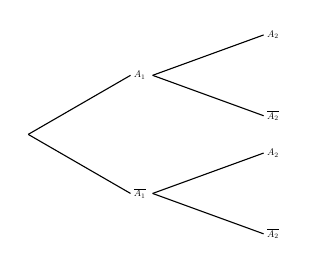
\begin{tikzpicture}
[scale=0.5]
\draw (0,0) -- (30:3) node [right, scale=0.35] {$A_1$} node [above, midway, rotate=30, scale=0.7] {};
\draw (0,0) -- (-30:3) node [right, scale=0.35] {$\overline{A_1}$} node [below, midway, rotate=-30, scale=0.7] {};
\draw (3.159807,1.5) -- ++(20:3) node [right, scale=0.35] {$A_2$} node [above, midway, rotate=20, scale=0.7] {};
\draw (3.159807,1.5) -- ++(-20:3) node [right, scale=0.35] {$\overline{A_2}$} node [below, midway, rotate=-20, scale=0.7] {};
\draw (3.159807,-1.5) -- ++(20:3) node [right, scale=0.35] {$A_2$} node [above, midway, rotate=20, scale=0.7] {};
\draw (3.159807,-1.5) -- ++(-20:3) node [right, scale=0.35] {$\overline{A_2}$} node [below, midway, rotate=-20, scale=0.7] {};
\end{tikzpicture}\end{center}
Figura 9.30: Ilustração das quatro configurações possíveis via diagrama de árvore

Em cada ramificação, assinalamos a respectiva probabilidade. Veja na figura 9.31, o diagrama de árvore com as respectivas probabilidades destacadas.
\begin{center}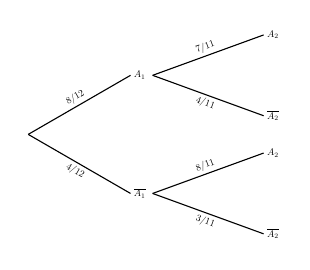
\begin{tikzpicture}
[scale=0.5]
\draw (0,0) -- (30:3) node [right, scale=0.35] {$A_1$} node [above, midway, rotate=30, scale=0.35] {8/12};
\draw (0,0) -- (-30:3) node [right, scale=0.35] {$\overline{A_1}$} node [below, midway, rotate=-30, scale=0.35] {4/12};
\draw (3.159807,1.5) -- ++(20:3) node [right, scale=0.35] {$A_2$} node [above, midway, rotate=20, scale=0.35] {7/11};
\draw (3.159807,1.5) -- ++(-20:3) node [right, scale=0.35] {$\overline{A_2}$} node [below, midway, rotate=-20, scale=0.35] {4/11};
\draw (3.159807,-1.5) -- ++(20:3) node [right, scale=0.35] {$A_2$} node [above, midway, rotate=20, scale=0.35] {8/11};
\draw (3.159807,-1.5) -- ++(-20:3) node [right, scale=0.35] {$\overline{A_2}$} node [below, midway, rotate=-20, scale=0.35] {3/11};
\end{tikzpicture}\end{center}
Figura 9.31: Diagrama de árvore do exemplo com as respectivas probabilidades

Na figura 9.32, destacam-se as quatro configurações possíveis e respectivas probabilidades.
\begin{center}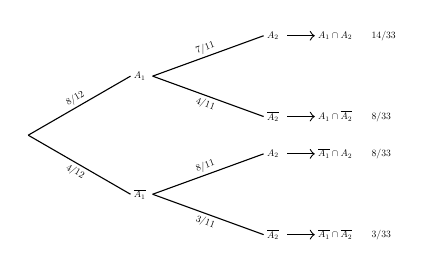
\begin{tikzpicture}
[scale=0.5]
\draw (0,0) -- (30:3) node [right, scale=0.35] {$A_1$} node [above, midway, rotate=30, scale=0.35] {8/12};
\draw (0,0) -- (-30:3) node [right, scale=0.35] {$\overline{A_1}$} node [below, midway, rotate=-30, scale=0.35] {4/12};
\draw (3.159807,1.5) -- ++(20:3) node [right, scale=0.35] {$A_2$} node [above, midway, rotate=20, scale=0.35] {7/11};
\draw (3.159807,1.5) -- ++(-20:3) node [right, scale=0.35] {$\overline{A_2}$} node [below, midway, rotate=-20, scale=0.35] {4/11};
\draw (3.159807,-1.5) -- ++(20:3) node [right, scale=0.35] {$A_2$} node [above, midway, rotate=20, scale=0.35] {8/11};
\draw (3.159807,-1.5) -- ++(-20:3) node [right, scale=0.35] {$\overline{A_2}$} node [below, midway, rotate=-20, scale=0.35] {3/11};
\draw [->] (6.57888,2.5260) -- ++(0:0.7) node [right, scale=0.35] {$A_1 \cap A_2 \qquad 14/33$};
\draw [->] (6.57888,0.4739) -- ++(0:0.7) node [right, scale=0.35]   {$A_1 \cap \overline{A_2} \qquad 8/33$};
\draw [->] (6.57888,-0.4739) -- ++(0:0.7) node [right, scale=0.35]   {$\overline{A_1} \cap A_2 \qquad 8/33$};
\draw [->] (6.57888,-2.5260) -- ++(0:0.7) node [right, scale=0.35]   {$\overline{A_1} \cap \overline{A_2} \qquad 3/33$};
\end{tikzpicture}\end{center}
Figura 9.32: Diagrama de árvore indicando os quatro casos possíveis após o sorteio

Logo, pela árvore, \(P(E)=\frac{8}{33}+\frac{8}{33}=\frac{16}{33}\).
\end{sphinxadmonition}


\subsection{Eventos Independentes}
\label{\detokenize{PE511-7:id3}}\label{\detokenize{PE511-7:eventos-independentes}}
Na Atividade \sphinxstyleemphasis{usio de óculos e sexo de estudantes}, concluímos que uso de óculos independe de gênero, pois  comparando as probabilidades incondicionais de ser do gênero feminino (0,55) e de ser do gênero masculino (0,45) com as probabilidades condicionais de ser do gênero feminino (0,545) e do gênero masculino (0,455) dado que usa óculos, percebe-se que elas são aproximadamente iguais. Na teoria, para que os eventos sejam independentes, essas probabilidades deveriam ser iguais. Na prática esse tipo de análise é usado em Estatística para avaliar a hipótese de independência entre dois eventos.
\begin{description}
\item[{Dois eventos \(A\) e \(B\) são ditos independentes se a ocorrência de um deles não muda a incerteza sobre a ocorrência do outro.\index{Dois eventos  e  são ditos independentes se a ocorrência de um deles não muda a incerteza sobre a ocorrência do outro.|textbf}}] \leavevmode\phantomsection\label{\detokenize{PE511-7:term-dois-eventos-e-sao-ditos-independentes-se-a-ocorrencia-de-um-deles-nao-muda-a-incerteza-sobre-a-ocorrencia-do-outro}}
\end{description}

Em símbolos, \(A\) e \(B\)  são ditos eventos independentes se \(P(A|B)=P(A)\), ou equivalentemente, se \(P(B|A)=P(B)\).

Decorre, da definição de probabilidade condicional,
\(P(A|B)=\frac{P(A\cap B)}{P(B)}\), que se \(A\) e \(B\)
são eventos independentes, então \(P(A\cap B)=P(A) \cdot P(B)\).

É preciso ter cuidado ao usar este último resultado. Se não sabemos que os eventos \(A\) e \(B\) são independentes, então devemos usar a regra da multiplicação, a saber, \(P(A\cap B)=P(B)\cdot P(A|B)\) que vale para quaisquer dois eventos.

Observe que há uma simetria no conceito de independência de tal modo que se
\(P(A|B)=P(A)\) , então \(P(B|A)=P(B)\).

De fato, se \(P(A|B)=P(A)\), segue que \(P(A\cap B)=P(A) \cdot P(B)\) e, assim,
\begin{equation*}
\begin{split}P(B|A)=\frac{P(A\cap B)}{P(A)}=\frac{P(A)\cdot P(B)}{P(A)}=P(B)\end{split}
\end{equation*}
\begin{sphinxadmonition}{note}{Exemplo: Eventos independentes versus eventos disjuntos}

Considere o experimento que consiste em lançar um dado honesto e, em seguida, lançar uma moeda honesta. Defina os eventos \(A:\) “ocorre uma face par” e \(B:\) “ocorre uma cara”.
\begin{enumerate}
\item {} 
\(A\) e \(B\) são eventos disjuntos?

\item {} 
\(A\) e \(B\) são eventos independentes?

\end{enumerate}

Observe que estamos lidando com um experimento sequencial de modo que os resultados possíveis envolvem a combinação de dois casos, a saber, número do dado e tipo de face da moeda. Como são seis números possíves para o dado e duas faces possíveis para a moeda, segue que o espaço amostral desse experimento consiste de 12 pares ordenados:

\(S=\{(1,ca),(1,co),(2,ca),(2,co),(3,ca),(3,co),(4,ca),(4,co),(5,ca),(5,co),(6,ca),(6,co)\}\)

Embora seja comum pensar que os eventos \(A\) e \(B\) são disjuntos, depois de descrever os elementos do espaço amostral é fácil perceber que \(A`e  `B\) não são disjuntos (\(A\cap B\neq \emptyset\)). De fato,

\(A=\{(2,ca),(2,co),(4,ca),(4,co),(6,ca),(6,co)\}\) tal que \(P(A)=\frac{6}{12}=0,5\)

\(B=\{(1,ca),(2,ca),(3,ca),(4,ca),(5,ca),(6,ca)\}\) tal que \(P(B)=\frac{6}{12}=0,5\)

\(A\cap B=\{(2,ca),(4,ca),(6,ca)\}\) tal que \(P(A\cap B)=\frac{3}{12}=\frac{1}{4}=0,25\)

É natural pensarmos que os lançamentos do dado e da moeda sejam independentes, pois o resultado de um não interfere no resultado de outro. Podemos confirmar esse raciocínio, observando que \(P(A\cap B)=0,25\) é igual ao produto das probabilidades incondicionais de \(A\) e de \(B\)  ambas iguais a 0,5.
\end{sphinxadmonition}

Do exemplo anterior vale destacar que, dados dois eventos com probabilidade positiva, não será possível que eles sejam ao mesmo tempo disjuntos e independentes.

\begin{sphinxadmonition}{note}{Exemplo: Eventos disjuntos versus eventos independentes}

Sejam \(A\) e \(B\) dois eventos em um espaço amostral \(S\) tais que \(P(A)>0\) e \(P(B)>0\).
\begin{enumerate}
\item {} 
Se \(A\) e \(B\) são eventos disjuntos, então \(A`e `B\) não são eventos independentes.

Se \(A\) e \(B\) são disjuntos, então \(P(A\cap B)=0\neq P(A)\cdot P(B)>0, pois `P(A)>0\) e \(P(B)>0\). Assim, \(A\) e \(B\) não são independentes.

\item {} 
Se \(A\) e \(B\) são eventos independentes, então \(A`e `B\) não são eventos disjuntos.

Se \(A\) e \(B\) são independentes, então \(P(A\cap B)=P(A)\cdot P(B)>0`o que implica que `A\cap B\neq \emptyset\). Logo, \(a\) e \(B\) não são disjuntos.

\end{enumerate}

Observe que a única situação em que se pode ter \(A\)  e \(B\)  simultaneamente disjuntos e independentes ocorre se um dos eventos \(A\) ou \(B\) tiver probabilidade nula.
\end{sphinxadmonition}

\begin{sphinxadmonition}{note}{Definição}

Três eventos \(A\), \(B\)  e  \(C\) são independentes se, e somente se, eles são dois a dois independentes e \(P(A\cap B\cap C)=P(A)\cdot P(B)\cdot P(C)\).
\end{sphinxadmonition}

\begin{sphinxadmonition}{note}{Exemplo: Três eventos dois a dois independentes que não são independentes}

Considere um dado em forma de tetraedro regular cujos números de suas faces são 1, 2, 3 e 4 (figura 9.33).
\begin{quote}
\phantomsection\label{\detokenize{PE511-7:id4}}
\begin{figure}[H]
\centering

\noindent\sphinxincludegraphics[width=200bp]{{tetraedro_dado}.png}
\label{\detokenize{PE511-7:id4}}\end{figure}

Figura 9.33: Dado em forma de tetraedro com a face 2 oculta
\end{quote}

Defina os eventos \(A=\{1,2\}\), \(B=\{1,3\}\) e \(C=\{1,4\}\).
\begin{enumerate}
\item {} 
Verifique que \(A\) e \(B\)  são eventos independentes.

\item {} 
Idem para \(A\) e \(C\).

\item {} 
Idem para \(B\) e \(C\).

\item {} 
Calcule \(P(A|B\cup C)\), compare o resultado obtido com \(P(A)\) e diga se \(A\) e \(B\cup C\) são eventos independentes.

\end{enumerate}

É fácil perceber que os eventos \(A\), \(B\) e \(C\) tomados dois a dois são independentes, pois a interseção entre dois dos três é sempre \(\{1\}\) cuja probabilidade é \(\frac{1}{4}\) e como cada um dos eventos \(A\), \(B\) e \(C\) têm probabilidade \(\frac{1}{2}\), segue que
\(P(A\cap B)=P(A)\cdot P(B)=\frac{1}{2}\cdot\frac{1}{2}=\frac{1}{4}\)

\(P(A\cap C)=P(A) \cdot P(C)=\frac{1}{2}\cdot\frac{1}{2}=\frac{1}{4}\) e

\(P(B\cap C)=P(B)\cdot P(C)=\frac{1}{2}\cdot\frac{1}{2}=\frac{1}{4}\).

Mas, \(P(A|B\cup C)=\frac{P(A\cap (BUC))}{P(B\cup C)}=\frac{P((A\cap B)\cup (A\cap C))}{P(B\cup C)}=\frac{1/4}{3/4}=\frac{1}{3}\neq P(A)\) e, portanto, \(A\) e \(B\cup C\)  não são independentes apesar de \(A\) e \(B\) serem independentes e de \(A\) e \(C\) serem indepedentes.

Portanto, se temos três eventos dois a dois independentes, isso não implicará que os três eventos sejam independentes.
\end{sphinxadmonition}


\practice{ Probabilidade Condicional}
\label{\detokenize{PE511-8:praticando-probabilidade-condicional}}\label{\detokenize{PE511-8::doc}}\begin{sphinxadmonition}{note}{Atividade}{desempenho de exames diagnósticos}
\label{ativ-especificidade-sensibilidade}

\begin{sphinxadmonition}{note}{Para o professor}

\sphinxstylestrong{Objetivo específico:} Reconhecer uma probabilidade condicional.

\sphinxstylestrong{Observações e sugestões:} Essa atividade envolve uma adaptação de uma questão do ENEM (2014).

\begin{sphinxadmonition}{note}{Resposta}

Defina \(A\): o evento ” a pessoa sorteada tem a doença X{}` e \(B\): o evento ” o resultado do teste da pessoa sorteada foi positivo”.
\begin{enumerate}
\item {} 
Entre os duzentos indivíduos, 100 têm a doença \(X\), logo \(P(A)=\frac{100}{200}=0,5\).

\item {} 
\(P(\bar{A})=1-0,5=0,5\).

\item {} 
\(P(A|B)=\frac{P(A\cap B)}{P(B)}=\frac{95}{110}\approx 0,864\).

\item {} 
\(P(A|\bar{B})=\frac{5}{90}\approx 0,056\).

\item {} 
Entre as 100 pessoas doentes, 95 resultados foram positivos, logo \(P(B|A)=0,95\).

\item {} 
Entre as 100 pessoas sadias, 85 resultados foram negativos, logo \(P(\bar{B}|\bar{A})=0,85\).

\item {} 
0,95 e 0,85, respectivamente, conforme os itens (c) e (d).

\end{enumerate}
\end{sphinxadmonition}
\end{sphinxadmonition}

Testes diagnósticos para detectar uma doença não são infalíveis. Para analisar o desempenho de um desses testes, realizam-se estudos em populações, contendo pessoas sãs e portadoras da doença.
\phantomsection\label{\detokenize{PE511-8:fig-coloque-aqui-o-nome}}
\begin{figure}[H]
\centering

\noindent\sphinxincludegraphics[width=200bp]{{amostras_sangue}.png}
\label{\detokenize{PE511-8:fig-coloque-aqui-o-nome}}\end{figure}

Figura 9.34: Amostras de sangue para realização de exame
\end{sphinxadmonition}

Quatro situações distintas podem ocorrer
\begin{enumerate}
\item {} 
a pessoa TEM a doença e o resultado do teste é POSITIVO.

\item {} 
a pessoa TEM a doença e o resultado do teste é NEGATIVO.

\item {} 
a pessoa NÃO TEM a doença e o resultado do teste é POSITIVO.

\item {} 
a pessoa NÃO TEM a doença e o resultado do teste é NEGATIVO.

\end{enumerate}

Observe que nas situações (b) e (c), o teste falha, pois deveria ser positivo quando a pessoa tem a doença e, negativo, quando a pessoa não tem a doença. Já nas situações (a) e (d) o teste acerta o diagnóstico.

Dois índices de desempenho para avaliação de um teste diagnóstico costumam ser usados: a sensibilidade e especificidade.

A \sphinxstylestrong{sensibilidade} é definida como a probabilidade de o resultado do teste ser POSITIVO, dado que a pessoa examinada tem a doença. Já a \sphinxstylestrong{especificidade} é a probabilidade do teste ser NEGATIVO, dado que a pessoa examinada não tem a doença.
\begin{quote}

O quadro a seguir refere-se a um teste diagnóstico para a doença \(X\), aplicado em uma amostra composta por duzentas pessoas, sendo 100 sadias e 100 portadoras da doença \(X\).


\begin{savenotes}\sphinxattablestart
\centering
\begin{tabulary}{\linewidth}[t]{|T|T|T|}
\hline

Resultado
do teste
&
doente
&
sadia
\\
\hline
Positivo
&
95
&
15
\\
\hline
Negativo
&
5
&
85
\\
\hline
\end{tabulary}
\par
\sphinxattableend\end{savenotes}

Uma pessoa entre as duzentas dessa amostra será sorteada.
\begin{enumerate}
\item {} 
Qual a probabilidade de ela tenha a doença \(X\)?

\item {} 
Qual a probabilidade de que ela NÃO tenha a doença \(X\)?

\item {} 
Se o resultado do teste da pessoa sorteada foi positivo, calcule a probabilidade de que ela tenha a doença.

\item {} 
Se o resultado do teste da pessoa sorteada foi negativo, calcule a probabilidade de que ela tenha a doença.

\item {} 
Sabendo que a pessoa sorteada tem a doença, qual a probabilidade de seu teste ter resultado positivo?

\item {} 
Sabendo que a pessoa sorteada  NÃO tem a doença, qual a probabilidade de seu teste ter resultado negativo?

\item {} 
Determine uma estimativa da sensibilidade e da especificidade desse teste, usando a informação do quadro acima.

\end{enumerate}
\end{quote}
\begin{sphinxadmonition}{note}{Atividade}{produção de peças}
\label{ativ-producao-de-pecas}

\begin{sphinxadmonition}{note}{Para o professor}

\sphinxstylestrong{Objetivo específico:} Aplicar a definição de probabilidade condicional para reconhecer eventos independentes e eventos dependentes.

\begin{sphinxadmonition}{note}{Resposta}

Defina os eventos \(A\):  “peça produzida pela máquina I” e \(B\): “peça defeituosa”. Observe que os respectivos eventos complementares são \(\bar{A}:\) “peça produzida pela máquina II”, pois são apenas duas máquinas e \(\bar{B}:\) “peça boa”, pois são apenas duas classificações das peças (boas ou defituosas).

Se os eventos são independentes, deve-se ter \(P(B|A)=P(B)\), por exemplo. Tem-se que \(P(A)=\frac{200}{200+600}=0,25\), \(P(B)=\frac{20}{800}=0,025\) e \(P(B|A)=\frac{P(A\cap B)}{P(A)}=\frac{5/800}{200/800}=\frac{1}{40}=0,025\). Logo, conlui-se que a produção de defeituosas é independente do tipo de máquina, pois \(P(B|A)=P(B)\).

Observe que tanto faz a escolha dos eventos máquina I ou máquina II e peça defeituosa ou peça boa. Por exemplo,

\(P(\bar{A})=\frac{3}{4}=0,75\), \(P(B)=\frac{20}{800}=0,025\) e \(P(\bar{B})=0,975\).
Além disso, \(P(\bar{A}|B)=0,75=P(\bar{A})\), \(P(A|\bar{B})=0,25=P(A)\), \(P(\bar{A}|\bar{B})=0,75=P(\bar{A})\).

De fato, essa propriedade não é um caso específico desse problema e ela é explorada na próxima atividade.
\end{sphinxadmonition}
\end{sphinxadmonition}
\phantomsection\label{\detokenize{PE511-8:id1}}
\begin{figure}[H]
\centering

\noindent\sphinxincludegraphics[width=200bp]{{fabricacao_pecas}.png}
\label{\detokenize{PE511-8:id1}}\end{figure}
\end{sphinxadmonition}

Figura 9.35: Produção de peças
\begin{quote}

Para fins de controle de qualidade das peças produzidas em uma fábrica, foram analisadas amostras de peças produzidas por máquinas diferentes. Os resultados obtidos estão resumidos no quadro a seguir.


\begin{savenotes}\sphinxattablestart
\centering
\begin{tabulary}{\linewidth}[t]{|T|T|T|}
\hline

Máquina
&
Defeituosas
&
Boas
\\
\hline
I
&
5
&
195
\\
\hline
II
&
15
&
585
\\
\hline
\end{tabulary}
\par
\sphinxattableend\end{savenotes}

Pela informação das amostras coletadas, há razão para se acreditar que a produção de defeituosas ou boas é independente do tipo de máquina utilizada na produção?
\end{quote}
\begin{sphinxadmonition}{note}{Atividade}{independência e complementariedade}
\label{ativ-independencia-e-complementaridade}

\begin{sphinxadmonition}{note}{Para o professor}

\sphinxstylestrong{Objetivo específico:} Aplicar o conceito de independência entre dois eventos para entender que o respectivos eventos complementares herdam essa a condição de eventos independentes.

\sphinxstylestrong{Observações e sugestões:} Essa atividade é um exercício teórico de dedução muito simples que revela uma propriedade importante entre eventos independentes: dada uma coleção de eventos independentes, se para alguns eventos (ou todos) considerarmos os seus complementares em vez do próprio, a coleção continua independente. Com fins de simplificação e não tornar o processo complicado, consideraremos nesta atividade apenas o caso para dois eventos independentes. Mas, de fato, o resultado vale para quaisquer coleções de eventos independentes.

\begin{sphinxadmonition}{note}{Resposta}

\begin{enumerate}
\item {} 
Por hipótese temos que \(P(A\cap B)=P(A)\cdot P(B)\), pois \(A\)  e \(B\)  são independentes. Queremos provar que \(\bar{A}\) e \(\bar{B}\) também são independentes, ou equivalentemente, que \(P(\bar{A}\cap\bar{B})=P(\bar{A})\cdot P(\bar{B})\).

\end{enumerate}

Pelas Leis de De Morgan trabalhadas em atividade anterior, sabemos que \(\bar{A}\cap \bar{B}=\overline{(A\cup B)}\). Portanto, usando a propriedade do evento complementar, podemos escrever \(P(\bar{A}\cap \bar{B})=1-P(A\cup B)\).

Mas, \(P(A\cup B)=P(A)+P(B)-P(A\cap B)=P(A)+P(B)-P(A)\cdot P(B)\) pela independência entre \(A\) e \(B\). Assim,

\(P(\bar{A}\cap \bar{B})=1-P(A)-P(B)+P(A)\cdot P(B)=\)
\(=1-P(A) -P(B)\cdot (1-P(A))=(1-P(A))\cdot (1-P(B))=P(\bar{A})\cdot P(\bar{B})\).
Portanto, se \(A\) e \(B\) são independentes, então \(\bar{A}\) e \(\bar{B}\)  também são independentes.
\begin{enumerate}
\item {} 
Por hipótese temos que \(P(A\cap B)=P(A)\cdot P(B)\), pois \(A\)  e \(B\)  são independentes. Queremos provar que \({A}\) e \(\bar{B}\) também são independentes, ou equivalentemente, que \(P({A}\cap\bar{B})=P({A})\cdot P(\bar{B})\). Observe que podemos escrever \(A=(A\cap B)\cup (A\cap \bar{B})\) com os dois eventos do lado direito sendo disjuntos. Assim, \(P(A)=P(A\cap B)+P(A\cap \bar{B})\) implicando que \(P(A\cap \bar{B})=P(A)-P(A\cap B)=P(A)-P(A)\cdot P(B)\) pela independedência de \(A\) e \(B\). Logo, \(P(A\cap \bar{B})=P(A)\cdot (1-P(B))=P(A)\cdot P(\bar{B})\) e, portanto, se \(A\) e \(B\)  são independentes, então \(A\) e \(\bar{B}\) também são.

\item {} 
Idem ao item anterior, bastando trocar de posição as letras \(A\)  e \(B\).

\end{enumerate}
\end{sphinxadmonition}
\end{sphinxadmonition}

Sejam \(A\) e \(B\) dois eventos independentes.  Mostre que os pares de eventos a seguir também são independentes:
\begin{enumerate}
\item {} 
\(\bar{A}\) e \(\bar{B}\);

\item {} 
\(A\) e \(\bar{B}\); e

\item {} 
\(\bar{A}\) e \(B\).

\end{enumerate}
\end{sphinxadmonition}
\begin{sphinxadmonition}{note}{Atividade}{escolha da chave correta}
\label{ativ-chaves}

\begin{sphinxadmonition}{note}{Para o professor}

\sphinxstylestrong{Objetivo específico:} Estender a regra da multiplicação para o caso de mais de dois eventos.

\begin{sphinxadmonition}{note}{Resposta}

\#. Sejam os eventos \(A_i\):  “o cadeado é aberto na \(i\)-ésima tentativa”, \(i=1,2,3\). Queremos calcular
\(P(\bar{A_1}\cap \bar{A_2}\cap A_3)\) , pois por hipótese o cadeado não foi aberto nem na primeira nem na segunda tentetiva.

\(P(\bar{A_1}\cap \bar{A_2}\cap A_3)=P(\bar{A_1})\cdot P(\bar{A_2}|\bar{A_1})\cdot P(A_3|\bar{A_1}\cap \bar{A_2})=\frac{4}{5}\cdot \frac{4}{5}\cdot \frac{1}{5}=\frac{16}{125}=0,128\). Essa solução pode ser visualizada por meio do diagrama de árvore, ilustrado na figura a seguir.
\begin{center}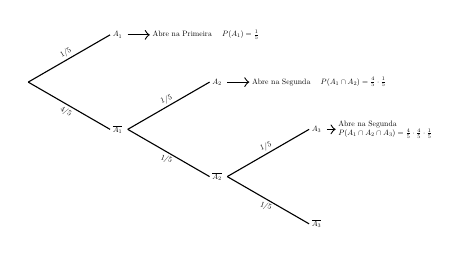
\begin{tikzpicture}
[scale=0.4]
\draw (0,0) -- (30:3) node [right, scale=0.28] {$A_1$} node [above, midway, rotate=30, scale=0.28] {1/5};
\draw (0,0) -- (-30:3) node [right, scale=0.28] {$\overline{A_1}$} node [below, midway, rotate=-30, scale=0.28] {4/5};
\draw [->] (3.159807,1.5) -- ++(0:0.7) node [right, scale=0.28] {Abre na Primeira $\quad P(A_1) = \frac{1}{5}$} ;
\draw (3.159807,-1.5) -- ++(30:3) node [right, scale=0.28] {$A_2$} node [above, midway, rotate=20, scale=0.28] {1/5};
\draw (3.159807,-1.5) -- ++(-30:3) node [right, scale=0.28] {$\overline{A_2}$} node [below, midway, rotate=-20, scale=0.28] {1/5};
\draw [->] (6.319614,0) -- ++(0:0.7) node [right, scale=0.28] {Abre na Segunda $\quad P(A_1 \cap A_2) = \frac{4}{5} \cdot \frac{1}{5}$} ;
\draw (6.319614,-3) -- ++(30:3) node [right, scale=0.28] {$A_3$} node [above, midway, rotate=20, scale=0.28] {1/5};
\draw (6.319614,-3) -- ++(-30:3) node [right, scale=0.28] {$\overline{A_3}$} node [below, midway, rotate=-20, scale=0.28] {1/5};
\draw [->, align=left] (9.479421,-1.5) -- ++(0:0.28) node [ right, scale=0.28] {Abre na Segunda \\ $P(A_1 \cap A_2 \cap A_3) = \frac{4}{5} \cdot \frac{4}{5} \cdot \frac{1}{5}$} ;
\end{tikzpicture}\end{center}\begin{enumerate}
\item {} 
Considerando agora o caso sem reposição tem-se

\end{enumerate}

\(P(\bar{A}_1\cap \bar{A}_2\cap A_3)=P(\bar{A}_1)\cdot P(\bar{A}_2|\bar{A}_1)\cdot P(A_3|\bar{A}_1\cap \bar{A}_2)=\frac{4}{5}\cdot \frac{3}{4}\cdot \frac{1}{3}=\frac{1}{5}=0,2\). Essa solução pode ser visualizada por meio do diagrama de árvore, ilustrado na figura a seguir.
\begin{center}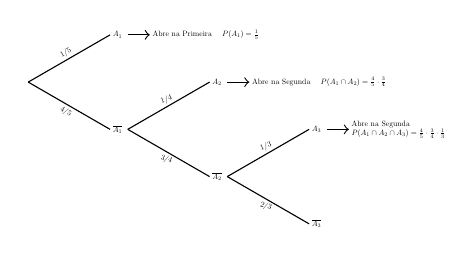
\begin{tikzpicture}
[scale=0.4]
\draw (0,0) -- (30:3) node [right, scale=0.28] {$A_1$} node [above, midway, rotate=30, scale=0.28] {1/5};
\draw (0,0) -- (-30:3) node [right, scale=0.28] {$\overline{A_1}$} node [below, midway, rotate=-30, scale=0.28] {4/5};
\draw [->] (3.159807,1.5) -- ++(0:0.7) node [right,  scale=0.28] {Abre na Primeira $\quad P(A_1) = \frac{1}{5}$} ;
\draw (3.159807,-1.5) -- ++(30:3) node [right, scale=0.28] {$A_2$} node [above, midway, rotate=20, scale=0.28] {1/4};
\draw (3.159807,-1.5) -- ++(-30:3) node [right, scale=0.28] {$\overline{A_2}$} node [below, midway, rotate=-20, scale=0.28] {3/4};
\draw [->] (6.319614,0) -- ++(0:0.7) node [right, scale=0.28] {Abre na Segunda $\quad P(A_1 \cap A_2) = \frac{4}{5} \cdot \frac{3}{4}$} ;
\draw (6.319614,-3) -- ++(30:3) node [right, scale=0.28] {$A_3$} node [above, midway, rotate=20, scale=0.28] {1/3};
\draw (6.319614,-3) -- ++(-30:3) node [right, scale=0.28] {$\overline{A_3}$} node [below, midway, rotate=-20, scale=0.28] {2/3};
\draw [->, align=left] (9.479421,-1.5) -- ++(0:0.7) node [ right, scale=0.28] {Abre na Segunda \\ $P(A_1 \cap A_2 \cap A_3) = \frac{4}{5} \cdot \frac{3}{4} \cdot \frac{1}{3}$} ;
\end{tikzpicture}\end{center}\end{sphinxadmonition}

Numa caixa há 5 chaves das quais apenas uma abre um cadeado.
\end{sphinxadmonition}
\phantomsection\label{\detokenize{PE511-8:id2}}
\begin{figure}[H]
\centering

\noindent\sphinxincludegraphics[width=200bp]{{chaves}.png}
\label{\detokenize{PE511-8:id2}}\end{figure}

Figura 9.36: Chaves e cadeado

Retirando-se chaves sequencialmente da caixa, qual a probabilidade de se abrir o cadeado apenas na terceira tentativa se:
\begin{enumerate}
\item {} 
a cada tentativa a chave extraída é recolocada na caixa?

\item {} 
a cada tentativa a chave extraída não é recolocada na caixa?

\item {} 
Em qual dos contextos (a) e (b) a probabilidade de se abrir a caixa é maior? Por quê?

\end{enumerate}
\end{sphinxadmonition}
\begin{sphinxadmonition}{note}{Atividade}{probabilidade total}
\label{ativ-tbayes}

\begin{sphinxadmonition}{note}{Para o professor}

\sphinxstylestrong{Objetivo específico:} Aplicar a definição de probabilidade condicional e propriedades da probabilidade para resolver um problema cuja solução faz uso do teorema de Bayes.

\sphinxstylestrong{Observações e sugestões} Com o material apresentado até aqui é possível resolver problemas cuja solução faz uso do teorema de Bayes. No entanto, optou-se nesse livro, a não apresentar a fórmula do teorema de Bayes, que só traz dificuldade para o aluno e, no entanto, é muito simples de ser deduzida na prática.

Teorema de Bayes: Sejam \(A_1, A_2, \cdots, A_n\) eventos tais que \(A_1\cup A_2\cup \cdots \cup A_n=S\) que são dois a dois disjuntos, ou seja, \(A_i\cap A_j=\emptyset\) sempre que \(i,j\in\{1,2,3,\cdots, n\}\) com \(i \neq j\). Seja \(B\subset S\). Então,

\(P(A_k|B)=\frac{P(A_k)\cdot P(B|A_k)}{\displaystyle{\sum^n_{i=1}}P(A_i)\cdot P(B|A_i)}\), \(k=1,2,\cdots, n\) .

\begin{sphinxadmonition}{note}{Resposta}

\begin{enumerate}
\item {} 
Defina os seguinte eventos \(A_1\): “bloco I é sorteado”, \(A_2\): “bloco II é sorteado” e  \(A_3\): “bloco III é sorteado”. Defina também o evento \(B:\) “um menor de até 12 anos é sorteado”. Observe que os eventos \(A_1\), \(A_2\) e \(A_3\) são disjuntos e que um menor sorteado pode ser de um, e somente um, dos três blocos. Logo, podemos escrever

\end{enumerate}

\(B=(A_1\cap B)\cup (A_2\cap B) \cup (A_3\cap B)\)

Como os eventos do lado direito da equação acima são disjuntos, tem-se

\(P(B)=P(A_1\cap B)+P(A_2\cap B)+P(A_3\cap B)\)

Usando-se a regra da multiplicação tem-se

\(P(B)=P(A_1)\cdot P(B|A_1)+P(A_2)\cdot P(B|A_2)+P(A_3)\cdot P(B|A_3)=\)

\(=\frac{1}{3}\cdot \frac{27}{180}+\frac{1}{3}\cdot\frac{36}{200}+\frac{1}{3}\cdot\frac{24}{120}=\frac{1}{20}+\frac{3}{50}+\frac{1}{15}=\frac{15+18+20}{300}=\frac{53}{300}\approx 0,177\).
\begin{enumerate}
\item {} 
Nesse item, deseja-se calcular a probabilidade condicional de ter ocorrido o evento \(A_2\), dado que ocorreu o evento \(B\), ou seja, \(P(A_2|B)\). Usando a definição de probabilidade condicional tem-se

\end{enumerate}

\(P(A_2|B)=\frac{P(A_2\cap B)}{P(B)}=\frac{P(A_2)\cdot P(B|A_2)}{53/300}=\frac{3}{50}\cdot\frac{300}{53}=\frac{18}{53}\approx 0,34\).
\end{sphinxadmonition}
\end{sphinxadmonition}

Em um condomínio há três prédios: bloco I, bloco II e bloco III. No bloco I há 180 moradores, no bloco II há 200 moradores e no bloco III há 120 moradores. Entre os moradores do bloco I, há 27 menores de até 12 anos. Entre os moradores do bloco II há 36 menores de até 12 anos. Entre os moradores do bloco III há 24 menores de até 12 anos. Um residente do condomínio será sorteado da seguinte forma: primeiro será sorteado um bloco, tendo os blocos probabilidades iguais.  Depois, um residente do bloco sorteado será escolhido ao acaso, usando-se um cadastro dos moradores do bloco. Pede-se calcular a probabilidade
\begin{enumerate}
\item {} 
a probabilidade de que a pessoa sorteada seja um menor de até 12 anos;

\item {} 
a probabilidade de ter sido sorteado o bloco II, sabendo que a pessoa sorteada é um menor de até 12 anos.

\end{enumerate}
\phantomsection\label{\detokenize{PE511-8:id3}}
\begin{figure}[H]
\centering

\noindent\sphinxincludegraphics[width=300bp]{{condominio_2}.png}
\label{\detokenize{PE511-8:id3}}\end{figure}

Figura 9.37: Condomínio com três blocos
\end{sphinxadmonition}


\know{ }
\label{\detokenize{PE511-A::doc}}\label{\detokenize{PE511-A:para-saber-mais}}
Em atividades anteriores foi sugerido lançar uma moeda repetidas vezes e registrar o resultado observado.  Veremos nesta seção como simular o lançamento de uma moeda um grande número de vezes com o auxílio da tecnologia.

Todos as linguagens de programação de computadores, planilhas e aplicativos costumam ter uma função interna usada para a geração de números aleatórios, na verdade, números pseudo-aleatórios, pois existe um mecanismo determinístico por trás da geração desses números.  Para mais detalhes sobre números (pseudo) aleatórios sugerimos assistir ao vídeo nesse  \sphinxhref{https://www.youtube.com/watch?v=f4sE1r3UL4E}{link}.

Nessa seção serão apresentadas algumas ferramentas úteis para fazer simulações de experimentos simples como o lançamento de uma ou mais moedas e  o lançamento de um ou mais dados.

Uma simulação de um experimento é um processo que tem o mesmo comportamento do experimento, de tal modo que resultados similares à realidade sejam gerados pelo processo.

As atividades a seguir consistirão em simulações de fenômenos aleatórios simples. Para sua realização será necessário o uso de tecnologia. A seguir, duas possibilidades serão detalhadas: as planilhas do  \sphinxhref{https://pt-br.libreoffice.org/}{LibreOffice} e do \sphinxhref{https://wiki.geogebra.org/en/Reference:GeoGebra\_Installation}{GeoGebra}.

A função \sphinxstyleemphasis{=ALEATÓRIOENTRE(1;N)} do LibreOffice, com \(N\) um número natural, produz um número do conjunto \(\{1,2,3,,\cdots, N\}\) de tal modo que a probabilidade de cada um dos números é dada por \(\frac{1}{N}\). Assim, ao usarmos \sphinxstyleemphasis{=ALEATÓRIOENTRE(1;2)}, o resultado será equivalente a sortear um número do conjunto \(\{1,2\}\) cada um com probabilidade igual a \(\frac{1}{2}\). Veja na figura 9.38 uma simulação de 20 números com essa propriedade, usando o LibreOffice.
\phantomsection\label{\detokenize{PE511-A:fig-coloque-aqui-o-nome}}
\begin{figure}[H]
\centering

\noindent\sphinxincludegraphics[width=400bp]{{libreoffice1}.png}
\label{\detokenize{PE511-A:fig-coloque-aqui-o-nome}}\end{figure}

Figura 9.38: Vinte simulações do sorteio dos números 1 e 2 com probabilidades iguais, usando o LibreOffice

Para simular os 20 números, basta digitar na célula A1 \sphinxstyleemphasis{=aleatórioentre(1;2)} e apertar a tecla \sphinxstyleemphasis{Enter}. Depois, posicione o cursor no canto esquerdo inferior da célula e arraste para baixo até a linha 20. Os 20 números gerados neste exemplo estão na coluna A da planilha. É possível gerar rapidamente, muito mais do que apenas 20 números.

Essa função, \sphinxstyleemphasis{aleatórioentre(1;2)} pode ser usada para simular o lançamento de uma moeda honesta, associando, por exemplo, o número 1 para a ocorrência de “cara” e, o número 2 para a ocorrência de  “coroa”, pois o modelo probabilístico da função \sphinxstyleemphasis{=aleatórioentre(1;2)} é tal que os dois números são gerados com probabilidades iguais. Assim, espera-se, em média, que as quantidades de números 1 (1’s) e de números 2 (2’s) sejam aproximadamente iguais.

Como fazer para obter de forma rápida essas quantidades, sem ter que contar um a um?

No LibreOffice a função \sphinxstyleemphasis{=cont.se(lista de células; número pesquisado)} faz essa contagem.

No exemplo anterior, a função \sphinxstyleemphasis{=cont.se(A1:A20;1)} irá retornar o número de 1’s encontrados nas células da coluna A das linhas 1 a 20. Já a  a função \sphinxstyleemphasis{=cont.se(A1:A20;2)} irá retornar o número de 2’s encontrados nas células da coluna A das linhas 1 a 20. Veja uma ilustração do uso da função na figura 9.39. Nessa figura, vemos que na simulação foram gerados doze (12) números 1 (caras) e oito (8) números 2 (coroas).
\phantomsection\label{\detokenize{PE511-A:id1}}
\begin{figure}[H]
\centering

\noindent\sphinxincludegraphics[width=400bp]{{Libreoffice2}.png}
\label{\detokenize{PE511-A:id1}}\end{figure}

Figura 9.39: Exemplo do uso da função cont.se do LibreOffice

No Geogebra as funções para realizar as mesmas tarefas são similares às utilizadas no LibreOffice. Veja na figura 9.40 a simulação do lançamento de uma moeda honesta 20 vezes, usando a função \sphinxstyleemphasis{=NúmeroAleatório(1,2)} do GeoGebra.
\phantomsection\label{\detokenize{PE511-A:id2}}
\begin{figure}[H]
\centering

\noindent\sphinxincludegraphics[width=400bp]{{GeoGebra1_1}.png}
\label{\detokenize{PE511-A:id2}}\end{figure}

Figura 9.40: GeoGebra: simulação de 20 lançamentos de uma moeda honesto, associando 1 para cara e 2 para coroa

Para a realização da contagem de caras e coroas, a função correspondente no GeoGebra é a função \sphinxstyleemphasis{ContarSe(números, células)}.

A quantidade de 1’s na coluna A das linhas 1 a 20 é dada por \sphinxstyleemphasis{=ContarSe(0\textless{}x\textless{}2,A1:A20)} que produzirá a quantidade de números inteiros no intervalo aberto {]}0,2{[} que ocorrem nas celas da coluna A das linhas 1 a 20 (A1:A20). Observe que o único número inteiro no intervalo aberto {]}0,2{[} é o número 1. Para contar a quantidade de 2’s na coluna A, devemos digitar \sphinxstyleemphasis{=ContarSe(1\textless{}x\textless{}3,A1:A20)}, lembrando que o único número inteiro no intervalo aberto {]}1,3{[} é o número 2.
\phantomsection\label{\detokenize{PE511-A:id3}}
\begin{figure}[H]
\centering

\noindent\sphinxincludegraphics[width=400bp]{{GeoGebra2_1}.png}
\label{\detokenize{PE511-A:id3}}\end{figure}

Figura 9.41: Geogebra: exemplo de uso da função \sphinxstyleemphasis{ContarSe}

Observe que na simulação realizada com o GeoGebra também foram obtidos doze números 1 (caras) e oito (8) números 2 (coroas). De fato, trata-se de mera coincidência, pois espera-se que, em média sejam produzidos a cada simulação, 10 caras.

\begin{sphinxadmonition}{note}{Exemplo: Simulação de um experimento cujo espaço amostral é equiprovável.}

Suponha que o espaço amostral \(S\) é dado por \(\{ 1,2,3,4,5,6,7,8,9,10,11,12\}\) e que os eventos elementares são equiprováveis.

A função do LibreOffice \sphinxstyleemphasis{=AleatórioEntre(1;12)} retornará com probabilidade \(\frac{1}{12}\) um dos elementos de \(S\).

A função do GeoGebra \sphinxstyleemphasis{=NúmeroAleatório(1,12)} retornará com probabilidade \(\frac{1}{12}\) um dos elementos de \(S\).
\phantomsection\label{\detokenize{PE511-A:id4}}
\begin{figure}[H]
\centering

\noindent\sphinxincludegraphics[width=400bp]{{geo1_1}.png}
\label{\detokenize{PE511-A:id4}}\end{figure}

Figura 9.42: Funções no Geogebra e LibreOffice

Observação:  Você poderá simular o lançamento de um dado ou de mais de um dado honesto e muitos outros experimentos simples, usando essas funções do Geogebra e do LibreOffice.
\end{sphinxadmonition}
\begin{sphinxadmonition}{note}{Atividade}{simulação do lançamento de uma moeda honesta}
\label{ativ-simulacao-moeda}

\begin{sphinxadmonition}{note}{Para o professor}

\sphinxstylestrong{Objetivo específico:} Aplicar o modelo probabilístico equiprovável e usar tecnologia para realizar simulações de um fenômeno aleatório.

\sphinxstylestrong{Observações e sugestões:} Essa atividade demanda o uso de tenologia. Sugere-se realizá-la em laboratório de informática. Sugere-se também que os alunos trabalhem em pequenos grupos de dois ou três alunos para cada computador disponível. As atividades poderão ser adaptadas de acordo com o conhecimento prévio dos estudantes. Nesssa atividade poderá ser usado o exemplo dado anteriormente, atribuindo um dos dois números para “cara” e, o outro, para “coroa”.
\begin{quote}

\begin{sphinxadmonition}{note}{Resposta}

\begin{enumerate}
\item {} 
Você pode realizar a simulação usando a planilha do Geogebra e a função \sphinxstyleemphasis{=NúmeroAleatório(1,2)} que irá gerar com probabilidades iguais ou o número 1 ou o número 2. Escolha um dos números para representar a ocorrência de cara e, o outro, para a ocorrência de coroa. Depois, arraste, copiando esta função para mais 19 células, obtendo as 20 simulações. Veja exemplo no início dessa seção. No GeoGebra ocorreram doze 1’s (caras) e oito 2’s (coroas) tal que a frequência relativa de caras observadas nessas 20 simulações foi \(\frac{12}{20}=0,6\). É claro que as respostas irão variar, dependendo da simulação. Mas, espera-se que o número de 1´’ (caras) obtidos oscile em torno de 10, pois a função produz os dois números com probabilidades iguais e geramos 20 números.

\item {} 
Idem ao item anterior, só que agora os números de células a serem considerados na planilha são 50, 100, 250 e 1000, respectivamente.

\item {} 
No preenchimento da tabela você deverá perceber que a medida que o número de simulações é maior, a frequência relativa de caras se aproxima da probabilidade teórica  de obter uma cara (0,5). Se de fato o gerador de números aleatórios do programa que você está usando é bom, esse é o resultado esperado. Por exemplo, em uma simulação com o Geogebra foram observadas as seguintes frequências relativas de caras conforme o número de lançamentos:

\end{enumerate}


\begin{savenotes}\sphinxattablestart
\centering
\begin{tabulary}{\linewidth}[t]{|T|T|}
\hline

Número de Observações
&
Frequência relativa de caras
\\
\hline
20
&
0,45
\\
\hline
50
&
0,58
\\
\hline
100
&
0,51
\\
\hline
250
&
0,52
\\
\hline
1000
&
0,49
\\
\hline
\end{tabulary}
\par
\sphinxattableend\end{savenotes}
\end{sphinxadmonition}
\end{quote}
\end{sphinxadmonition}

Deseja-se simular o lançamento de uma moeda honesta uma grande quantidade de vezes e comparar a frequência relativa de caras com a probabilidade teórica 0,5 de obter uma cara quando a moeda é honesta.
\phantomsection\label{\detokenize{PE511-A:id5}}
\begin{figure}[H]
\centering

\noindent\sphinxincludegraphics[width=100bp]{{lancamento_moeda}.png}
\label{\detokenize{PE511-A:id5}}\end{figure}
\begin{enumerate}
\item {} 
Usando o GeoGebra ou algum outro recurso tecnológico, simule 20 lançamentos da moeda e observe a quantidade de caras, calculando a frequência relativa.

\item {} 
Repita a simulação para 50, 100, 250 e 1000 lançamentos da moeda.

\item {} 
Complete o quadro a seguir e comente sobre os resultados obtidos.

\end{enumerate}


\begin{savenotes}\sphinxattablestart
\centering
\begin{tabulary}{\linewidth}[t]{|T|T|}
\hline

Número de Observações
&
Frequência relativa de caras
\\
\hline
20
&\\
\hline
50
&\\
\hline
100
&\\
\hline
250
&\\
\hline
1000
&\\
\hline
\end{tabulary}
\par
\sphinxattableend\end{savenotes}
\end{sphinxadmonition}
\begin{sphinxadmonition}{note}{Atividade}{simulação do lançamento de um dado honesto}
\label{ativ-simulacao-dado}

\begin{sphinxadmonition}{note}{Para o professor}

\sphinxstylestrong{Objetivo específico:} Aplicar o modelo probabilístico equiprovável e usar tecnologia para realizar simulações de um fenômeno aleatório.

\sphinxstylestrong{Observações e sugestões:} Essa atividade demanda o uso de tenologia. Sugere-se realizá-la em laboratório de informática. Sugere-se também que os alunos trabalhem em pequenos grupos de dois ou três alunos para cada computador disponível. As atividades poderão ser adaptadas de acordo com o conhecimento prévio dos estudantes. Nesssa atividade poderá ser usado exemplo dado anteriormente, gerando-se um número aleatório entre 1 e 6 e, depois, contando as quantidades obtidas de cada face.
\begin{quote}

\begin{sphinxadmonition}{note}{Resposta}

\begin{enumerate}
\item {} 
Você pode realizar a simulação usando a planilha do GeoGebra e a função \sphinxstyleemphasis{=NúmeroAleatório(1,6)} na célula A1. Essa função retornará, com probabilidades iguais, um entre os números 1,2,3,4,5 e 6. Depois, arraste, copiando esta função para mais 29 células A2 até A30, obtendo as 30 simulações. Veja exemplo no início dessa seção. Depois use a função \sphinxstyleemphasis{=ContarSe(5\textless{}x\textless{}7,A1:A30)}. É claro que as respostas irão variar, dependendo da simulação. Mas, espera-se que o número de faces “6” obtidas oscile em torno de 5, pois a função gera o número 6 com probabilidade 1/6 e assim, em média espera-se obter \(30\cdot \frac{1}{6}=5\) dígitos 6.

\item {} 
Idem ao item anterior, só que agora o número de células a ser considerado na planilha será 60, 120, 300 e 1500.

\item {} 
No preenchimento da tabela você deverá perceber que a medida que o número de simulações é maior, a frequência relativa de faces 6 se aproxima da probabilidade teórica  de obter uma face 6 (\(\approx 0,167\)). Se de fato o gerador de números aleatórios do programa que você está usando é bom, esse é o resultado esperado. Por exemplo, em uma simulação com o GeoGebra foram observadas as seguintes frequências relativas de faces 6 conforme o número de lançamentos:

\end{enumerate}


\begin{savenotes}\sphinxattablestart
\centering
\begin{tabulary}{\linewidth}[t]{|T|T|}
\hline

Número de Observações
&
Frequência relativa de 6’s
\\
\hline
30
&
0,17
\\
\hline
60
&
0,18
\\
\hline
120
&
0,18
\\
\hline
300
&
0,16
\\
\hline
1500
&
0,17
\\
\hline
\end{tabulary}
\par
\sphinxattableend\end{savenotes}
\end{sphinxadmonition}
\end{quote}
\end{sphinxadmonition}

Deseja-se simular o lançamento de um dado honesto uma grande quantidade de vezes e comparar a frequência relativa de faces “6” com a probabilidade teórica \(\frac{1}{6}\approx 0,167\) de obter uma face “6” quando o dado é honesto.
\phantomsection\label{\detokenize{PE511-A:id6}}
\begin{figure}[H]
\centering

\noindent\sphinxincludegraphics[width=200bp]{{lancamento_dado}.png}
\label{\detokenize{PE511-A:id6}}\end{figure}
\begin{enumerate}
\item {} 
Usando o GeoGebra ou algum outro recurso tecnológico, simule 30 lançamentos do dado e observe a quantidade de faces “6” obtidas, calculando a frequência relativa.

\item {} 
Repita a simulação para 60, 120, 300 e 1500 lançamentos do dado.

\item {} 
Complete o quadro a seguir e comente sobre os resultados que você obteve.

\end{enumerate}


\begin{savenotes}\sphinxattablestart
\centering
\begin{tabulary}{\linewidth}[t]{|T|T|}
\hline

Número de Observações
&
Frequência relativa de 6’s
\\
\hline
30
&\\
\hline
60
&\\
\hline
120
&\\
\hline
300
&\\
\hline
1500
&\\
\hline
\end{tabulary}
\par
\sphinxattableend\end{savenotes}
\end{sphinxadmonition}
\begin{sphinxadmonition}{note}{Atividade}{simulação do lançamento de um dado desequilibrado}
\label{ativ-simulacao-dado-desequilibrado}

\begin{sphinxadmonition}{note}{Para o professor}

\sphinxstylestrong{Objetivo específico:} Aplicar modelo probabilístico não equiprovável e usar tecnologia para realizar simulações de um fenômeno aleatório.

\sphinxstylestrong{Observações e sugestões:} Nessa atividade será proposta a simulação de um dado desequilibrado de tal modo que as faces não ocorrem com probabilidades iguais. Inicialmente será necessária uma discussão sobre com os alunos desequilibrados. Em particular, nessa atividade será suposto que a probabilidade da face é proporcional ao número da face.
Assim, a primeira pergunta envolverá obter as probabilidades de cada face. Fazendo \(P(\{i\})=k\cdot i\) em que \(i=1,2,3,4,5,6\) e \(k\) é a constante de proporcionalidade, lembre com os alunos a segunda regra básica de que \(P(S)=1\) e que \(\{1\}\cup \{2\}\cup \cdots \cup \{6\}=S\). Além disso, como os eventos elementares são disjuntos segue que \(1=P(\{1\})+P(\{2\})+\cdots+P(\{6\})=k+2k+3k+4k+5k+6k=21k\) tal que \(k=\frac{1}{21}.\) Depois dessa dedução será necessária uma discussão sobre como usar o gerador de números aleatórios para simular os resultados desse dado, para finalmente realizar a simulação de um número aleatório entre 1 e 21 e atribuido o 1 à face 1, depois o 2 e o 3 à face 2, o 4, o 5 e o 6 à face 3, o 7, o 8, o 9 e o 10 à face 4, o 11, o 12, o 13, o 14 e o 15 à face 5 e, finalmente, o 16, o 17, o 18, o 19, o 20 e o 21 à face 6. Leve o aluno a observar que desse modo estaremos respeitando as probabilidades desiguais, a saber, 1/21 para a face 1, 2/21 para a face 2, …, 6/21 para a face 6.
\begin{quote}

\begin{sphinxadmonition}{note}{Resposta}

\begin{enumerate}
\item {} 
Você pode realizar a simulação usando a planilha do Geogebra e a função \sphinxstyleemphasis{=NúmeroAleatório(1,21)} na célula A1. Essa função retornará, com probabilidades iguais, um entre os números 1,2,3,4,5, …,21. Depois, arraste, copiando esta função para mais 41 células A2 até A42, obtendo as 42 simulações. Observe que nesse caso, você deverá usar apenas um número para atribuir à ocorrência da face 1, dois números para a face 2, e assim por diante, com seis números para a face 6. Se consideraros os seis últimos, a saber, 21, 20, 19, 18, 17 e 16, use a função \sphinxstyleemphasis{=ContarSe(15\textless{}x\textless{}22,A1:A42)}, para obter a quantidade de faces 6 obtidas nos 42 lançamentos. É claro que as respostas irão variar de um para outro. Mas, espera-se que o número de faces “6” obtidas oscile em torno de 12, pois a probabilidade de gerar uma face “6”  com esse procedimento é \(\frac{6}{21}\approx 0,286\) e estamos simulando 42 lançamentos.

\item {} 
Idem ao item anterior, só que agora o número de células a ser considerado na planilha será 210, 630, 840 e 1680.

\item {} 
No preenchimento da tabela você deverá perceber que a medida que o número de simulações é maior, a frequência relativa de faces 6 se aproxima da probabilidade teórica  de obter uma face 6 (\(\approx 0,286\)). Se de fato o gerador de números aleatórios do programa que você está usando é bom, esse é o resultado esperado. Por exemplo, em uma simulação com o GeoGebra foram obserdas as seguintes frequências relativas de faces 6 conforme o número de lançamentos:

\end{enumerate}


\begin{savenotes}\sphinxattablestart
\centering
\begin{tabulary}{\linewidth}[t]{|T|T|}
\hline

Número de Observações
&
Frequência relativa de 6’s
\\
\hline
42
&
0,29
\\
\hline
84
&
0,31
\\
\hline
210
&
0,30
\\
\hline
630
&
0,28
\\
\hline
840
&
0,29
\\
\hline
1680
&
0,29
\\
\hline
\end{tabulary}
\par
\sphinxattableend\end{savenotes}
\end{sphinxadmonition}
\end{quote}
\end{sphinxadmonition}

Um dado é desequilibrado quando suas faces ocorrem com probabilidades desiguais. Suponha que um dado seja desequilibrado de tal modo que a probabilidade de ocorrer cada uma de suas faces, entre os números 1, 2, 3, 4, 5 e 6, sejam proporcionais aos respectivos números das faces.
\begin{enumerate}
\item {} 
Determine as probabilidades de cada face no caso desse dado.

\item {} 
Usando as funções de geração de números aleatórios, simule o lançamento desse dado 42 vezes e compare a frequência relativa de faces 6 obtidas com a probabilidade teórica da face 6 obtida no item anterior.

\item {} 
Repita o item anterior para 84, 210, 630, 840 e 1680 lançamentos do dado desequilibrado e registre o número de vezes que você obteve a face 6.

\item {} 
Complete a tabela a seguir e comente sobre os resultados que você obteve.

\end{enumerate}


\begin{savenotes}\sphinxattablestart
\centering
\begin{tabulary}{\linewidth}[t]{|T|T|}
\hline

Número de Observações
&
Frequência relativa de 6’s
\\
\hline
42
&\\
\hline
210
&\\
\hline
630
&\\
\hline
840
&\\
\hline
1680
&\\
\hline
\end{tabulary}
\par
\sphinxattableend\end{savenotes}
\end{sphinxadmonition}
\begin{sphinxadmonition}{note}{Atividade}{simulação do lançamento de um dado diferente}
\label{ativ-simulacao-dado-especial}

\begin{sphinxadmonition}{note}{Para o professor}

\sphinxstylestrong{Objetivo específico:} Aplicar modelo probabilístico e usar tecnologia para realizar simulações de um fenômeno aleatório.

\sphinxstylestrong{Observações e sugestões:} Nessa atividade será proposta a simulação de um dado diferente. Apesar das faces ocorrerem com probabilidades iguais, esse dados tem registrado em suas faces o número 1 em uma delas, o núermo 2 em duas delas e o número 3 em três delas. Discuta com seus alunos como adaptar a função de geração de números aleatórios para simular resultados de lançamentos desse dado. É fácil perceber, da atividade anterior que a probabilidade de 3 é 3/6, de 2 é 2/6 e, de 1, 1/6.
\begin{quote}

\begin{sphinxadmonition}{note}{Resposta}

\begin{enumerate}
\item {} 
A probabilidade de obter face 1 é dada por \(\frac{1}{6}\), de obter face 2 é dada por \(\frac{2}{6}\) e, de obter face 3 é dada por \(\frac{3}{6}\), pois o dado é equilibrado, mas há uma face 1, duas faces 2 e três faces 3.

\item {} 
Você pode realizar a simulação usando a planilha do Geogebra e a função \sphinxstyleemphasis{=NúmeroAleatório(1,6)} na célula A1. Essa função retornará, com probabilidades iguais, um entre os números 1,2,3,4,5,6. Depois, arraste, copiando esta função para mais 29 células A2 até A30, obtendo as 30 simulações. Observe que nesse caso, você deverá atribuir apenas um número para a ocorrência da face 1, dois números para a face 2 e  três números para a face 3. Se considerarmos os números 2 e 3 para a ocorrência de face 2, use a função \sphinxstyleemphasis{=ContarSe(1\textless{}x\textless{}4,A1:A30)}. É claro que as respostas irão variar, dependendo da simulação. Mas, espera-se que o número de faces “2” obtidas oscile em torno de 10, pois a probabilidade de obter uma face “2” é 2/6 e estamos simulando 30 lançamentos.

\item {} 
Idem ao item anterior, só que agora o número de células a ser considerado na planilha será 300, 600, 900 e 1800.

\item {} 
No preenchimento da tabela você deverá perceber que a medida que o número de simulações é maior, a frequência relativa de faces 2 se aproxima da probabilidade teórica  de obter uma face 2 (\(\approx 0,333\)). Se de fato o gerador de números aleatórios do programa que você está usando é bom, esse é o resultado esperado. Por exemplo, em uma simulação com o GeoGebra foram observadas as seguintes frequências relativas de faces 2 conforme o número de lançamentos:

\end{enumerate}


\begin{savenotes}\sphinxattablestart
\centering
\begin{tabulary}{\linewidth}[t]{|T|T|}
\hline

Número de Observações
&
Frequência relativa de 2’s
\\
\hline
30
&
0,40
\\
\hline
300
&
0,36
\\
\hline
600
&
0,35
\\
\hline
900
&
0,34
\\
\hline
1800
&
0,34
\\
\hline
\end{tabulary}
\par
\sphinxattableend\end{savenotes}
\end{sphinxadmonition}
\end{quote}
\end{sphinxadmonition}

Um dado é equilibrado, mas suas faces foram pintadas de tal modo que há uma face 1, duas faces 2 e três faces 3.
\begin{enumerate}
\item {} 
Determine as probabilidades de se obter face 1, face 2 e face 3 com esse dado.

\item {} 
Usando as funções de geração de números aleatórios, simule o lançamento desse dado 30 vezes e compare a frequência relativa de faces 2 obtidas com a probabilidade teórica da face 2 obtida no item anterior.

\item {} 
Repita o item anterior para 300, 600, 900 e 1800 lançamentos do dado equilibrado e registre o número de vezes que você obteve a face 2.

\item {} 
Complete a tabela a seguir e comente sobre os resultados que você obteve.

\end{enumerate}


\begin{savenotes}\sphinxattablestart
\centering
\begin{tabulary}{\linewidth}[t]{|T|T|}
\hline

Número de Observações
&
Frequência relativa de 2’s
\\
\hline
30
&\\
\hline
300
&\\
\hline
600
&\\
\hline
900
&\\
\hline
1800
&\\
\hline
\end{tabulary}
\par
\sphinxattableend\end{savenotes}
\end{sphinxadmonition}

\begin{sphinxadmonition}{note}{Teorema: Lei dos Grandes Números}

À medida que um experimento é repetido várias vezes, a probabilidade dada pela frequência relativa de um evento tende a se aproximar da probabilidade teórica.
\end{sphinxadmonition}

A lei dos grandes números nos diz que as estimativas da probabilidade de um evento dadas pelas frequências relativas tendem a ficar melhores com mais observações. Esse resultado, como já comentado anteriormente, é a base teórica para a interpretação frequentista de probabilidade. Veja na figura 9.17, uma ilustração da Lei dos Grandes Números.

\begin{sphinxadmonition}{note}{Exemplo: Cálculo de probabilidade, usando simulação}

Deseja-se calcular a probabilidade de se obter pelo menos uma face 6, quando um dado honesto é lançado quatro vezes.

Definindo \(A\) como sendo o evento ocorreu pelo menos um seis nos quatro lançamentos, então \(\bar{A}\) é o evento nenhum 6 ocorreu nos quatro lançamentos.

Nesse caso, podemos usar a propriedade do evento complementar para calcular \(P(A)=1-P(\bar{A})\).
O evento \(\bar{A}\)  ocorre se, e somente se, em cada um dos quatro lançamentos não ocorre face 6. Como os lançamentos são independentes, a probabilidade de não ocorrer face 6 nos quatro lançamentos será dada por
\begin{equation*}
\begin{split}\frac{5}{6}\cdot \frac{5}{6}\cdot \frac{5}{6}\cdot \frac{5}{6}=\left (\frac{5}{6}\right )^4\approx 0,48\end{split}
\end{equation*}
Assim \(P(A) \approx 1- 0,48=0,52\).

Vamos estimar essa probabilidade, usando a Lei dos Grandes Números com o auxílio do GeoGebra.

Para simular o experimento podemos usar a função \sphinxstyleemphasis{=Número Aleatório(1,6)} nas céluas A1 até A4.
\phantomsection\label{\detokenize{PE511-A:id7}}
\begin{figure}[H]
\centering

\noindent\sphinxincludegraphics[width=400bp]{{GeoGebra_e1}.png}
\label{\detokenize{PE511-A:id7}}\end{figure}

Figura 9.43: Simulação de quatro lançamento de um dado com o GeoGebra

Na cela B4 usaremos a função \sphinxstyleemphasis{=ContarSe(5\textless{}x\textless{}7,A1:A4)} para obter o número de faces 6 obtidas.
\phantomsection\label{\detokenize{PE511-A:id8}}
\begin{figure}[H]
\centering

\noindent\sphinxincludegraphics[width=400bp]{{GeoGebra_e2}.png}
\label{\detokenize{PE511-A:id8}}\end{figure}

Figura 9.44: Contagem do número de faces 6’s obtidas, usando o GeoGebra

Depois, marque as células A1:B4 e arraste-as até a linha 400, de modo a repetir 100 vezes esse experimento.
\phantomsection\label{\detokenize{PE511-A:id9}}
\begin{figure}[H]
\centering

\noindent\sphinxincludegraphics[width=400bp]{{GeoGebra_e3_1}.png}
\label{\detokenize{PE511-A:id9}}\end{figure}

Figura 9.45: Simulação de 100 experimentos (lançar um dado 4 vezes), usando o GeoGebra

Vamos então usar a função \sphinxstyleemphasis{ContarSe(-1\textless{}x\textless{}1,B1:B400)} para obter a quantidade de zeros, ou seja, o número de repetições do experimento em que a face 6 não ocorreu.
\phantomsection\label{\detokenize{PE511-A:id10}}
\begin{figure}[H]
\centering

\noindent\sphinxincludegraphics[width=400bp]{{GeoGebra_e4_1}.png}
\label{\detokenize{PE511-A:id10}}\end{figure}

Figura 9.46: Contagem do número de ocorrências do evento “nenhuma face 6”

Observe que foram 43 ocorrências sem nenhuma face 6 de modo que nessa simulação a probabilidade estimada de obter pelo menos um 6 é dada por \(1-0,43=0,57\). Observe que essa estimativa ficou ligeiramente afastada da probabiliade teórica (\(\approx 0,52\)).

Duplicando o número de repetições do experimento, espera-se obter uma estimativa mais próxima da probabilidade teórica. Veja na figura 9.47 um resultado, usando o GeoGebra. Agora, com 200 repetições, a estimativa  foi 0,54 e, portanto, mais perto da probabilidade teórica.
\phantomsection\label{\detokenize{PE511-A:id11}}
\begin{figure}[H]
\centering

\noindent\sphinxincludegraphics[width=400bp]{{GeoGebra_e5}.png}
\label{\detokenize{PE511-A:id11}}\end{figure}

Figura 9.47: Simulação de 200 experimentos (lançar um dado 4 vezes), usando o GeoGebra
\end{sphinxadmonition}


\exercise
\label{\detokenize{PE511-E:exercicios}}\label{\detokenize{PE511-E::doc}}
\(1.\) (Pisa) Imagine que tenha sido apresentado um documentário sobre terremotos, no qual é dito com que frequência ocorrem  e como podem ser previstos. Nesse documentário, um geólogo afirmou: “nos próximos  20 anos, a chance de um terremoto acontecer na cidade de Zed é de duas em três.”
\begin{quote}

Qual das sentenças a seguir reflete o significado da afirmação feita pelo geólogo?
\begin{enumerate}
\item {} 
Como \(\frac{2}{3}\cdot 20\approx 13,3\); entre 13 e 14 anos a partir de agora, ocorrerá um terremoto na cidade de Zed.

\item {} 
Como \(\frac{2}{3}\) é maior do que \(\frac{1}{2}\), temos certeza de que ocorrerá um terremoto na cidade de Zed em algum momento nos próximos 20 anos.

\item {} 
A probabilidade de ocorrer algum terremoto na cidade de Zed em algum momento nos próximos 20 anos é maior do que a probabilidade de ele não ocorrer.

\item {} 
Não se pode dizer sobre o que irá acontecer, pois ninguém sabe quando um terremoto ocorrerá.

\end{enumerate}
\end{quote}

\(2.\) (Pisa) Para dado dia, a previsão do tempo afirma que, das 12h às 18h, a chance de ocorrência de chuva é de 30\%.
\begin{quote}

Assinale a alternativa que corresponde à melhor interpretação dessa previsão do tempo.
\begin{enumerate}
\item {} 
Em 30\% da área à qual a previsão se refere haverá chuva.

\item {} 
em 30\% de 6 horas, ou seja, durante o total de 108 minutos, haverá chuva.

\item {} 
Em relação às pessoas da área à qual a previsão se refere, pode-se afirmar que 30 a cada 100 pessoas pegarão chuva.

\item {} 
Se a mesma previsão fosse dada para 100 dias, em cerca de 30 desses 100 dias haveria chuva.

\item {} 
A quantidade de chuva será 30\% da intensidade de uma forte precipitação (medida como “chuva por unidade de tempo”).

\end{enumerate}
\end{quote}

\(3.\) Sabe-se que a probabilidade de que um casal com três filhos tenha duas meninas é \(\frac{3}{8}\). Com base nessa afirmação, responda:
\begin{enumerate}
\item {} 
Observando-se ao acaso 160 casais com três filhos, quantos casais você espera que tenham duas meninas?

\item {} 
E em 400 casais com três filhos?

\item {} 
É correto afirmar que se observarmos 80 casais com três filhos, exatamente 30 casais terão duas meninas? Por quê?

\end{enumerate}

\(4.\) Nas situações a seguir indique a interpretação de probabilidade, entre as interpretações clássica, frequentista e subjetiva, que melhor se encaixa para a designação de probabilidades.
\begin{enumerate}
\item {} 
Um dado honesto é lançado três vezes, deseja-se calcular a probabilidade de se obter pelo menos duas faces pares.

\item {} 
Um gerente de banco deseja avaliar a probabilidade de um cliente esperar mais de 30 minutos para ser atendido em um dia comum.

\item {} 
Deseja-se avaliar a probabilidade de você se tornar um \sphinxstyleemphasis{Youtuber} de sucesso no próximo ano.

\end{enumerate}

\(5.\) Em uma escola de Ensino Médio há dois turnos: manhã e tarde. Nesta escola há alunos que praticam atividade física fora do horário escolar e alunos que não praticam. Um aluno dessa escola será sorteado. Defina os seguintes eventos \(A:\) “o aluno sorteado é do turno da manhã” e \(B:\) “o aluno sorteado pratica atividade física fora do horário escolar”. Descreva em palavras os eventos
\begin{enumerate}
\item {} 
\(A\cup B\)

\item {} 
\(A\cap B\)

\item {} 
\(\bar{A}\cap \bar{B}\)

\item {} 
\(\overline{A\cap B}\)

\end{enumerate}

\(6.\) É sorteado um aluno de uma turma de um curso de Inglês na qual há somente alunos de 15 anos, 16 anos e 17 anos completos. Sabe-se que a  probabilidade de o aluno selecionado ter 15 anos é igual a 0,3 e ter 17 anos é igual a 0,2.
Determine a probabilidade de o aluno sorteado
\begin{enumerate}
\item {} 
ter idade maior do que 16 anos.

\item {} 
ter 16 anos.

\item {} 
ter pelo menos 15 anos.

\item {} 
ter 15 ou 16 anos.

\end{enumerate}

\(7.\) Um posto de coleta de sangue fez um lavantamento das fichas de 500 doadores, obtendo as seguintes frequências relativas por tipo sanguíneor e fator Rh.
\begin{quote}


\begin{savenotes}\sphinxattablestart
\centering
\begin{tabulary}{\linewidth}[t]{|T|T|T|T|}
\hline

tipo
&
Rh+
&
Rh-
&
total
\\
\hline
O
&
0,32
&
0,08
&
0,40
\\
\hline
A
&
0,20
&
0,10
&
0,30
\\
\hline
AB
&
0,16
&
0,04
&
0,20
\\
\hline
B
&
0,07
&
0,03
&
0,10
\\
\hline
total
&
0,75
&
0,25
&
1,00
\\
\hline
\end{tabulary}
\par
\sphinxattableend\end{savenotes}

Supondo que o comportamento desses doadores reflita o comportamento da população da região do posto de coleta que contém 1 milhão de pessoas, pede-se calcular, de forma aproximada, o número de pessoas nessa população que
\begin{enumerate}
\item {} 
tenha fator Rh-;

\item {} 
tenha sangue tipo A;

\item {} 
tenha sangue tipo AB com fator Rh+;

\item {} 
não tenha sangue tipo O.

\item {} 
não tenha sangue tipo O, sabendo que tem fator Rh+.

\item {} 
não tenha sangue tipo O, sabendo que tem fator Rh-.

\end{enumerate}
\end{quote}

\(8.\) (UERJ-EQ1-2011) Uma fábrica produz sucos com os seguintes sabores: uva, pêssego e laranja. Considere uma caixa com 12 garrafas desses sucos, sendo quatro de cada sabor. Retirando-se ao acaso duas garrafas dessa caixa, a probabilidade de que ambas as garrafas contenham suco com o mesmo saber equivale a:
\begin{enumerate}
\item {} 
9,1\%

\item {} 
18,2\%

\item {} 
27,3\%

\item {} 
36,4\%

\end{enumerate}

\(9.\) (UERJ-EQ1-2012-adaptada) Três modelos de aparelhos de ar condicionado I, II e III, de diferentes potências são produzidos por determinado fabricante. Uma consulta sobre intenção de troca de modelo foi realizada com 1000 usuários desses produtos. No quadro a seguir estão indicados os tipos de modelos que os usuários possuem e se eles pretendem mudar para outro modelo ou não.

Dos 400 que possuem o modelo I, 50 não pretendem mudar de modelo, 150 pretendem mudar para o II e 250 para o III. Dos 400 que possuem o modelo II, 100 não pretendem mudar e 300 pretendem mudar para o III. E, dos 200 que possuem o modelo III, nenhum deles tem intenção de mudar.

Escolhendo-se aleatoriamente um dos usuários consultados, a probabilidade de que ele não pretenda trocar seu modelo de ar condicionado é:
\begin{enumerate}
\item {} 
20\%

\item {} 
35\%

\item {} 
40\%

\item {} 
65\%

\end{enumerate}

\(10.\) (UERJ-EQ2-2013) Em uma escola, 20\% dos alunos de uma turma marcaram a opção correta de uma questão de múltipla escolha que possui quatro alternativas de resposta. Ode demais alunos marcaram uma das quatro opções ao acaso. Verificando-se as respostas de dois alunos quaisquer dessa turma, a probabilidade de que exatamente um tenha marcado a opção correta é:
\begin{enumerate}
\item {} 
0,48

\item {} 
0,40

\item {} 
0,36

\item {} 
0,25

\end{enumerate}

\(11.\) (ENEM) Um aluno de determinada escola será escolhido por sorteio para representa-la em certa atividade. A escola tem dois turnos. No diurno há 300 alunos, distribuídos em 10 turmas de 30 alunos cada. No noturno há 240 alunos, distribuídos em 6 turmas de 40 alunos cada. Em vez do sorteio direto, envolvendo os 540 alunos, foram propostos dois outros métodos de sorteio.
MÉTODO I: Escolher ao acaso um dos turnos e, a seguir, sortear um dos alunos do turno escolhido.
MÉTODO II: Escolher ao acaso uma das 16 turmas e, a seguir, sortear um dos alunos dessa turma.
Sobre os métodos I e II é correto afirmar:
\begin{enumerate}
\item {} 
Em ambos os métodos, todos os alunos têm a mesma chance de serem sorteados.

\item {} 
No método I, todos os alunos têm a mesma chance de serem sorteados, mas no método II a chance de um aluno do diurno ser sorteado é maior do que a de um aluno do noturno.

\item {} 
No método II, todos os alunos têm a mesma chance de serem sorteados, mas no método I a chance de um aluno do diurno ser sorteado é maior do que a de um aluno do noturno.

\item {} 
No método I, a chance de um aluno do noturno ser sorteado é maior do que a chance de um aluno do diurno, enquanto no método II ocorre o contrário.

\item {} 
Em ambos os métodos, a chance de um aluno do diurno ser sorteado é maior do que a de um aluno do noturno.

\end{enumerate}

\(12.\) (ENEM) Um município de 628 km2 é atendido por duas emissoras de rádio cujas antenas A e B alcançam um raio de 10 km do município, conforme mostra a figura 9.48:
\begin{center}\begin{tikzpicture}
[scale=0.5]
\draw [color=secundario!70, fill=primario!70] (2,3) -- (3,3) -- (3.55,2.16);
\draw [dashed, ] (0,0) -- (0,3);
\draw [] (0,3) -- (3,3) -- (5,0) -- (0,0);
\draw [, fill=primario!70] (2,3) arc (-180:-56.1:1);
\draw [, fill=primario!70] (5,0) -- (4,0) arc (180:123.9:1) -- cycle;
\node [above right, scale=0.35] at (3,3) {$A$};
\node [above, scale=0.3] at (2.5,3) {10 km};
\node [rotate=-56.1, above, scale=0.3] at (4.718, 0.395) {10 km};
\node [below right, scale=0.35] at (5,0) {$B$};
\node [below, scale=0.3] at (4.5,0) {10 km};
\draw [very thin] (0,0) rectangle (0.2,0.2);
\draw [very thin] (0,3) rectangle (0.2,2.8);
\node [ponto, scale=0.4] at (0.1,0.1) {};
\node [ponto, scale=0.4] at (0.1,2.9) {};
\draw plot [smooth, tension=1] coordinates {(1,3) (0.75,1.5) (1.5,0)};
\node [right, scale=0.25] at (1,1.5) {Município};
\end{tikzpicture}\end{center}
Figura 9.48: Planta do município

Para orçar um contrato publicitário, uma agência precisa avaliar a probabilidade que um morador tem de, circulando livremente pelo município, encontrar-se na área de alcance de pelo menos uma das emissoras. Essa probabilidade é de aproximadamente:
\begin{enumerate}
\item {} 
20\%

\item {} 
25\%

\item {} 
30\%

\item {} 
35\%

\item {} 
40\%

\end{enumerate}

\(13.\) (ENEM - 2017) Um morador de uma região metropolitana tem 50\% de probabilidade de atrasar-se para o trabalho quando chove na região; caso não chova, sua probabilidade de atraso é de 25\%. Para um determinado dia, o serviço de meteorologia estima em 30\% a probabilidade da ocorrência de chuva nessa região.

Qual é probabilidade de esse morador se atrasar para o serviço no dia para o qual foi dada a estimativa de chuva?
\begin{enumerate}
\item {} 
0,075

\item {} 
0,150

\item {} 
0,325

\item {} 
0,600

\item {} 
0,800

\end{enumerate}

\(14.\) (ENEM - 2017) Numa avenida existem 10 semáforos. Por causa de uma pane no sistema, os semáforos ficaram sem controle durante uma hora, e fixaram suas luzes unicamente em verde ou vermelho. Os semáforos funcionam de forma independente; a probabilidade de acusar cor verde é de \(\frac{2}{3}\) e a de acusar cor vermelha é de \(\frac{1}{3}\). Uma pessoa percorreu a pé toda essa avenida durante o período da pane, observando a cor da luz de cada um desses semáforos.

Qual é a probabilidade de que esta pessoa tenha observado exatamente um sinal na cor verde?
\begin{enumerate}
\item {} 
\(\frac{10\cdot 2}{3^{10}}\)

\item {} 
\(\frac{10\cdot 2^9}{3^{10}}\)

\item {} 
\(\frac{2^{10}}{3^{100}}\)

\item {} 
\(\frac{2^{90}}{3^{100}}\)

\item {} 
\(\frac{2}{3^{10}}\)

\end{enumerate}

\(15.\) (UFPR) Durante um surto de gripe, 25\% dos funcionários de uma empresa contraíram essa doença. Dentre os que contraíram gripe, 80\% apresentaram febre. Constatou-se também que 8\% dos funcionários apresentaram febre por outros motivos naquele período. Qual a probabilidade de que um funcionário dessa empresa, selecionado ao acaso, tenha apresentado febre durante o surto de gripe?
\begin{enumerate}
\item {} 
20\%

\item {} 
26\%

\item {} 
28\%

\item {} 
33\%

\item {} 
35\%

\end{enumerate}

\(16.\) (ENEM) Numa escola com 1200 alunos foi realizada uma pesquisa sobre o conhecimento desses em duas línguas estrangeiras: inglês e espanhol. Nessa pesquisa, constatou-se que 600 alunos falam inglês, 500 falam espanhol e 300 não falam qualquer um desses idiomas.

Escolhendo-se um aluno dessa escola ao acaso e sabendo-se que ele não fala inglês, qual a probabilidade de que esse aluno fale espanhol?
\begin{enumerate}
\item {} 
\(\frac{1}{2}\)

\item {} 
\(\frac{5}{8}\)

\item {} 
\(\frac{1}{4}\)

\item {} 
\(\frac{ 5}{6}\)

\item {} 
\(\frac{5}{14}\)

\end{enumerate}

\(17.\) (ENEM) O psicólogo de uma empresa aplica um teste para analisar a aptidão de um candidato a determinado cargo. O teste consiste em uma série de perguntas cujas respostas devem ser verdadeiro ou falso e termina quando o psicólogo fizer a décima pergunta ou quando o candidato der a segunda resposta errada, Com base em testes anteriores, o psicólogo sabe que a probabilidade de o candidato errar qualquer uma das respostas é 0,2. A probabilidade do teste terminar na quinta pergunta é:
\begin{enumerate}
\item {} 
0,02048

\item {} 
0,08192

\item {} 
0,24000

\item {} 
0,40960

\item {} 
0,49152

\end{enumerate}

\(18.\) De um lote contendo 20 lâmpadas das quais 5 são defeituosas, deseja-se extrair duas lâmpadas e testá-las sequencialmente.
\begin{quote}
\begin{enumerate}
\item {} 
Se as lâmpadas são extraídas sem reposição ao lote, responda:
\begin{enumerate}
\item {} 
Qual a probabilidade de se extrair duas defeituosas?

\item {} 
Qual a probabilidade de se extrair duas boas?

\item {} 
Qual a probabilidade de se extrair uma boa e uma defeituosa em qualquer ordem?

\end{enumerate}

\item {} 
Se as lâmpadas são extraídas com reposição ao lote, responda:

\end{enumerate}
\begin{enumerate}
\item {} 
Qual a probabilidade de se extrair duas defeituosas?

\item {} 
Qual a probabilidade de se extrair duas boas?

\item {} 
Qual a probabilidade de se extrair uma boa e uma defeituosa em qualquer ordem?

\end{enumerate}
\end{quote}

\begin{sphinxadmonition}{note}{Respostas}

\(1.\) A sentença C é a única correta. Se a probabilidade de ocorrer um terremoto nos próximos 20 anos é 2/3, então a probabilidade de não ocorrer um terremoto nos próximos 20 anos é 1-2/3=1/3 (regra do evento complementar) tal que é duas vezes mais provável ele ocorrer do que não ocorrer nos próximos 20 anos. A alternativa A não faz sentido, pois considera a fração 2/3 de 20 anos, quando a interpretação correta da probabilidade é a de que se pudessemos observar 60 períodos similares de 20 anos na cidade de Zed, em cerca de 40 desses perídos haveria um terremoto. A alternativa B também está errada, pois uma medida de probabilidade maior que zero e menor que 1 não nos fornece “certeza”. A alternativa D també está incorrreta, pois sabe-se que há maior chance de ocorrer um terremoto do que não ocorrer, apesar de não sermos capazes de afirtmar se ele irá ocorrer ou não e quando ele irá ocorrer.

\(2.\) A alternativa que melhor corresponde à afirmação é D. A probabilidade indica uma taxa de ocorrência do evento, caso ele seja repetido um grande número de vezes. Assim, se observarmos 100 dias similares, em cerca de 30 desses dias irá chover. Observe que esse número de fato pode não ser exatamente 30, apenas espera-se que ele seja próximo de 30. Lembre-se que se você lançar uma moeda honesta 20 vezes, não necessariamente irá observar 10 caras, mesmo sabendo que a probabilidade de ocorrer cara em cada lançamento é 50\%.

\(3.\) Se a probabilidade de um casal com três filhos ter duas meninas é 3/8,
\begin{enumerate}
\item {} 
espera-se que entre 160 casais com três filhos cerca de \(160\cdot \frac{3}{8}=60\) casais tenham duas meninas.

\item {} 
espera-se que entre 400 casais com três filhos cerca de \(400\cdot \frac{3}{8}=150\) casais tenham duas meninas.

\item {} 
Não, pois espera-se que entre 80 casais com três filhos cerca de \(80\cdot \frac{3}{8}=30\) casais tenham duas meninas, podendo ocorrer um número de casais diferente de 30.

\end{enumerate}

\(4.\) As interpretações mais adequadas são
\begin{enumerate}
\item {} 
clássica, pois sendo o dado honesto atribuem-se probabiliades iguais para cada uma das 6 faces possíveis, a saber, 1/6.

\item {} 
frequentista. Nesse caso, a partir da observação de um grande número de tempos de espera, o gerente poderá usar a frequência relativa de ocorrência dos tempos de espera de mais de 30 minutos como a probabilidade do evento “esperar mais de 30 inutos para ser atendido”.

\item {} 
subjetiva.

\end{enumerate}

\(5.\)  Observe que os eventos complementares são \(\bar{A}:\) “ser do turno da tarde” e \(\bar{B}:\) “não pratica atividade física fora do horário escolar”. Descrições
\begin{enumerate}
\item {} 
Ocorre pelo menos um dos eventos entre “ser do turno da manhã” \sphinxstylestrong{ou} “praticar atividade física fora do horário escolar”, podendo ocorrer apenas um dos dois ou os dois simultaneamente.

\item {} 
Ocorrem os dois eventos “ser do turno da manhã” \sphinxstylestrong{e} “praticar atividade física fora do horário escolar” simultaneamente.

\item {} 
Ocorrem os dois eventos “ser do turno da tarde” \sphinxstylestrong{e} “não praticar atividade física fora do horário escolar” simultaneamente.

\item {} 
Observe que pelas Leis de De Morgan \(\overline{A\cap B}=\bar{A}\cup \bar{B}\) tal que uma descrição para esse evento é Ocorre pelo menos um dos eventos entre “ser do turno da tarde” \sphinxstylestrong{ou} “não praticar atividade física fora do horário escolar”, podendo ocorrer apenas um dos dois ou os dois simultaneamente.

\end{enumerate}

\(6.\) Sejam os eventos \(A:\) “ter 15 anos”, \(B:\) “ter 16 anos” e \(C:\) “ter 17 anos”. Como só há essas três idades, segue que \(S=A\cup B\cup C\) e como \(A\), \(B\) e \(C\)  são disjuntos, tem-se
\(1=P(S)=P(A)+P(B)+P(C)\). Sabe-se que \(P(A)=0,3\) e \(P(C)=0,2\), logo \(P(B)=1-0,3-0,2=0,5\).
\begin{enumerate}
\item {} 
\(P(C)=0,2\)

\item {} 
\(P(B)=0,5\).

\item {} 
\(P(S)=1\).

\item {} 
Como \(A\) e \(B\) são disjuntos, tem-se \(P(A\cup B)=P(A)+P(B)=0,3+0,5=0,8\).

\end{enumerate}

\(7.\) Definindo o evento \(R:\) “ter Rh+” tal que \(\bar{R}:\) “ter Rh-” e usando os símbolos do tipo de sangue, tem-se
\begin{enumerate}
\item {} 
Como \(P(R)=0,75\), segue que o número esperado de pessoas com fator Rh+ é \(1.000.000\cdot 0,75=750.000\)

\item {} 
Como \(P(A)=0,30\), segue que o número esperado de pessoas  sangue tipo \(A\) é 300 mil.

\item {} 
Como \(P(AB\cap R)=0,16\), o número esperado de pessoas com tipo \(AB\) é 160 mil.

\item {} 
Como \(P(\bar{O})=1-0,40=0,60\), o número esperado de pessoas que não têm tipo \(O\) é 600 mil.

\item {} 
Como \(P(\bar{O}|R)=\frac{0,75-0,32}{0,75}\approx 0,57\), o número de  esperado de pessoas com fator Rh+ que têm sangue tipo \(O\) é \(0,57\cdot 750.000=427.500\).

\item {} 
Como \(P(\bar{O}|\bar{R})=\frac{0,25-0,08}{0,25}=0,68\), o número esperado de pessoas que não têm sangue tipo \(O`entre as pessoas com fator Rh- é `0,68\cdot 250.000=170.000\).

\end{enumerate}

\(8.\) Opção correta: (C)

Defina os eventos U1 e U2 para suco de uva na primeira seleção e suco de uva na segunda seleção. Similarmente, defina os eventos L1 e L2 e P1 e P2 para os sabores laranja e pêssego, respectivamente. Deseja-se calcular a probabilidade de que os dois sucos selecionados sejam do mesmo sabor, \(P((U1\cap U2)\cup (L1\cap L2) \cup (P1\cap P2))=P(U1\cap U2)+P(L1\cap L2)+P(P1\cap P2)\), pois os eventos são disjuntos. Usando a regra da multiplicação tem-se que \(P(U1\cap U2)=P(U1)\cdot P(U2|U1)=\frac{4}{12}\cdot\frac{3}{11}=\frac{1}{11}\). Como as quantidades de sucos dos tr\textasciitilde{}es sabores são iguais, segue que a resposta é \(3\cdot \frac{1}{11}=\frac{3}{11}\approx 0,273=27,3%\).

Essa solução é facilmente visualisada, usando-se o diagrama de árvore ilustrado na figura a seguir.
\begin{center}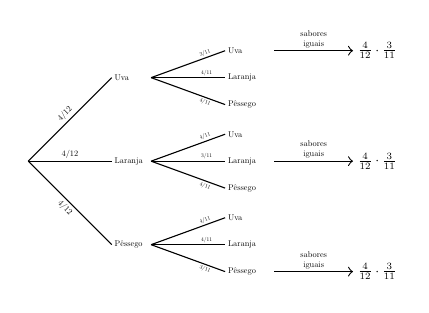
\begin{tikzpicture}
[scale=0.5]
\draw (0,0) -- (45:3) node [right, scale=0.3 ] {Uva} node [midway, above, scale=0.3, rotate=45] {4/12};
\draw (0,0) -- (-45:3) node [right, scale=0.3] {Pêssego} node [midway, below, scale=0.3, rotate=-45] {4/12};
\draw (0,0) -- (2.12132,0) node [right, scale = 0.3] {Laranja} node [midway, above, scale=0.3] {4/12};
\draw (3.12132,2.12132) -- ++(20:2) node [right, scale=0.3 ] {Uva} node [near end, above, scale=0.2, rotate=20] {3/11};
\draw (3.12132,2.12132) -- ++(0:1.8793) node [right, scale = 0.3]  {Laranja} node [near end, above, scale=0.2] {4/11};
\draw (3.12132,2.12132) -- ++(-20:2) node [right, scale=0.3] {Pêssego} node [near end, below, scale=0.2, rotate=-20] {4/11};
\draw (3.12132,0) -- ++(20:2) node [right, scale=0.3 ] {Uva} node [near end, above, scale=0.2, rotate=20] {4/11};
\draw (3.12132,0) -- ++(0:1.8793) node [right, scale = 0.3] {Laranja} node [near end, above, scale=0.2] {3/11};
\draw (3.12132,0) -- ++(-20:2) node [right, scale=0.3] {Pêssego} node [near end, below, scale=0.2, rotate=-20] {4/11};
\draw (3.12132,-2.12132) -- ++(20:2) node [right, scale=0.3 ] {Uva} node [near end, above, scale=0.2, rotate=20] {4/11};
\draw (3.12132,-2.12132) -- ++(0:1.8793) node [right, scale = 0.3] {Laranja}  node [near end, above, scale=0.2] {4/11};
\draw (3.12132,-2.12132) -- ++(-20:2) node [right, scale=0.3] {Pêssego} node [near end, below, scale=0.2, rotate=-20] {3/11};
\draw [->] (6.250062,0) -- ++(0:2) node [above, midway, align=center,scale=0.3] {sabores\\iguais} node [right, scale=0.5] {$\frac{4}{12} \cdot \frac{3}{11}$};
\draw [->] (6.250062,2.8053) -- ++(0:2) node [above, midway, align=center,scale=0.3] {sabores\\iguais} node [right, scale=0.5] {$\frac{4}{12} \cdot \frac{3}{11}$};
\draw [->] (6.250062,-2.8053) -- ++(0:2) node [above, midway, align=center,scale=0.3] {sabores\\iguais} node [right, scale=0.5] {$\frac{4}{12} \cdot \frac{3}{11}$};
\end{tikzpicture}\end{center}
\(9.\) Opção correta: (B)

Basta verificar que dos 1000 consumidores pesquisados \(50+100+200=350\) não pretendem mudar de modelo.

\(10.\) Opção correta (A)

Primeiro será necessário calcular a probabilidade de um aluno qualquer dessa turma acertar a questão. Temos que 20\% dos alunos a acertam com probabilidade 1, mas 80\% chutam, acertando com probabilidade \(\frac{1}{4}\), pois há quatro opções de resposta. Assim, a probabilidade de um aluno dessa turma acertar a questão é dada por \(0,2\cdot 1+0,8\cdot \frac{1}{4}=0,4\).

Usando o diagrama de árvore, podemos escrever para os dois alunos selecionados:
\begin{center}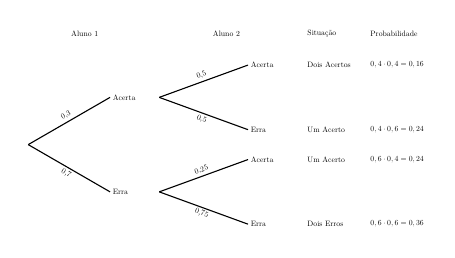
\begin{tikzpicture}
[scale=0.4]
\draw (0,0) -- (30:3) node [right, scale=0.28] {Acerta} node [above, midway, rotate=30, scale=0.28] {0,3};
\draw (0,0) -- (-30:3) node [right, scale=0.28] {Erra} node [below, midway, rotate=-30, scale=0.28] {0,7};
\draw (4.159807,1.5) -- ++(20:3) node [right, scale=0.28] {Acerta} node [above, midway, rotate=20, scale=0.28] {0,5};
\draw (4.159807,1.5) -- ++(-20:3) node [right, scale=0.28] {Erra} node [below, midway, rotate=-20, scale=0.28] {0,5};
\draw (4.159807,-1.5) -- ++(20:3) node [right, scale=0.28] {Acerta} node [above, midway, rotate=20, scale=0.28] {0,25};
\draw (4.159807,-1.5) -- ++(-20:3) node [right, scale=0.28] {Erra} node [below, midway, rotate=-20, scale=0.28] {0,75};
\node [right, scale=0.28] at (5.77888,3.5260) {Aluno 2};
\node [right, scale=0.28] at (1.27888,3.5260) {Aluno 1};
\node [right, scale=0.28] at (8.77888,3.5260) {Situação};
\node [right, scale=0.28] at (8.77888,2.5260) {Dois Acertos};
\node [right, scale=0.28] at (8.77888,0.4739) {Um Acerto};
\node [right, scale=0.28] at (8.77888,-0.4739) {Um Acerto};
\node [right, scale=0.28] at (8.77888,-2.5260) {Dois Erros};
\node [right, scale=0.28] at (10.77888,3.5260) {Probabilidade};
\node [right, scale=0.28] at (10.77888,2.5260) {$0,4 \cdot 0,4=0,16$};
\node [right, scale=0.28] at (10.77888,0.4739) {$0,4 \cdot 0,6=0,24$};
\node [right, scale=0.28] at (10.77888,-0.4739) {$0,6 \cdot 0,4=0,24$};
\node [right, scale=0.28] at (10.77888,-2.5260) {$0,6 \cdot 0,6=0,36$};
\end{tikzpicture}\end{center}
Logo, a probabilidade de que exatamente um aluno tenha marcado a opçãocorreta é dada por \(0,24+0,24=0,48.\)

\(11.\)  Opção correta: (D)

No método I, a probabilidade de selecionar um aluno do diurno será dada pela probabilidade de selecionar o turno diurno (1/2) vezes a probabilidade de selelcionar um aluno do diurno (1/300), ou seja, será dada por \(\frac{1}{600}\). Já a probabilidade de selecionar um aluno do noturno será dada por \(\frac{1}{2}\cdot \frac{1}{240}=\frac{1}{480}\). Assim, no método I, a probabilidade de selecionar um aluno do noturno é maior do que a probabilidade de selecionar um aluno do diurno. Portanto, as alternativas (a), (b), (c) e (d) são falsas.

No método II, a probabilidade de selecionar um aluno do diurno é dada por \(\frac{10}{16}\cdot\frac{1}{30}=\frac{1}{48}=\frac{20}{960}\). Já a probabilidade de selecionar um aluno do noturno é \(\frac{6}{16}\cdot \frac{1}{40}=\frac{3}{320}=\frac{9}{960}\). Assim, no método II, a probabilidade de selecionar um aluno do noturno é menor do que a probabilidade de selecionar um aluno do diurno. Portanto, a alternativa (d) está correta.

\(12.\) Opção correta: (B)

Para calcular a soma das áreas dos setores circulares na figura dada é necessário conhecer os respectivos ângulos centrais. No entanto, basta conhecer a soma dos ângulos centrais, que pela figura do trapézio implica que ela é 180 graus tal que os dois setores juntos podem formar a semi-circunfer\textasciitilde{}encia de raio 10 km. Logo, a probabilidade é dada por \(\frac{10^2\pi/2}{628}\approx \frac{314}{2\cdot 628} =0,25.\)

\(13.\) Opção correta: C

Usando o diagrama de árvore ilustrado na figura a seguir
\begin{center}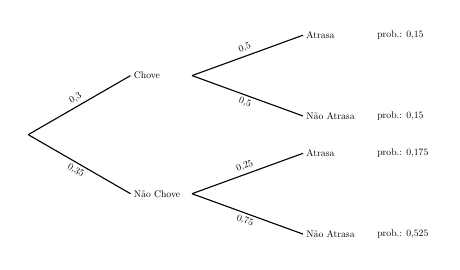
\begin{tikzpicture}
[scale=0.5]
\draw (0,0) -- (30:3) node [right, scale=0.35] {Chove} node [above, midway, rotate=30, scale=0.35] {0,3};
\draw (0,0) -- (-30:3) node [right, scale=0.35] {Não Chove} node [below, midway, rotate=-30, scale=0.35] {0,35};
\draw (4.159807,1.5) -- ++(20:3) node [right, scale=0.35] {Atrasa} node [above, midway, rotate=20, scale=0.35] {0,5};
\draw (4.159807,1.5) -- ++(-20:3) node [right, scale=0.35] {Não Atrasa} node [below, midway, rotate=-20, scale=0.35] {0,5};
\draw (4.159807,-1.5) -- ++(20:3) node [right, scale=0.35] {Atrasa} node [above, midway, rotate=20, scale=0.35] {0,25};
\draw (4.159807,-1.5) -- ++(-20:3) node [right, scale=0.35] {Não Atrasa} node [below, midway, rotate=-20, scale=0.35] {0,75};
\node [right, scale=0.35] at (8.77888,2.5260) {prob.: 0,15};
\node [right, scale=0.35] at (8.77888,0.4739) {prob.: 0,15};
\node [right, scale=0.35] at (8.77888,-0.4739) {prob.: 0,175};
\node [right, scale=0.35] at (8.77888,-2.5260) {prob.: 0,525};
\end{tikzpicture}\end{center}
tem-se que a probabilidade de atraso é dada por \(0,15+0,175=0,325.\)

Alternativamente, definindo \(A\) como o evento se atrasar e \(C\) como o evento chover, deseja-se calcular \(P(A)\). Mas, \(A=(A\cap C) \cup (A\cap \bar{C})\) com os dois eventos do lado esquerdo da igualdade disjuntos. Logo, \(P(A)=P(A\cap C)+P(A\cap \bar{C})=P(C)\cdot P(A|C)+P(\bar{C})\cdot P(A|\bar{C})=0,3\cdot 0,5+0,7\cdot 0,25=0,325\).

\(14.\) Opção correta (A)

Primeiro observe que existem 10 eventos possíveis que levam a observar apenas um semáforo verde, a saber, pode ser o primeiro ou o segundo, ou o terceiro e assim por diante até o décimo. Em seguida, observe que esses eventos são disjuntos de modo que a probabilidade desejada pode ser calculada pela soma das probabilidades desses 10 eventos ou, como elas são iguais, pelo produto da probabilidade de apenas a primeira ser verde por 10. Finalmente, pela independência, observe que qualquer que seja o evento a probabilidade é dada por \(\frac{2}{3}\cdot \frac{1}{3} \cdots \frac{1}{3}=\frac{2}{3}\cdot \left (\frac{1}{3}\right )^9=\frac{2}{3^{10}}\). Assim a probabilidade solicitada é \(\frac{10\cdot 2}{3^{10}}\).

\(15.\) Opção correta: (C)

Observe o diagramma de Venn a seguir com as informações do enunciado. Lembre que 80\% de 25\% corresponde a 20\%.
\begin{center}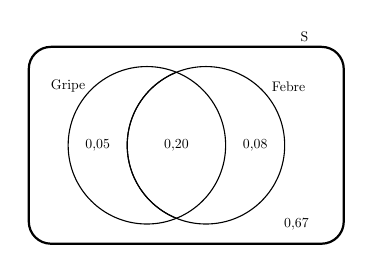
\begin{tikzpicture}
[scale=0.5]
\node [scale=0.5] at (7,5.25) {S};
\draw [ thick,rounded corners=8pt, -] (0,-0) -- (0,5) -- (8,5) -- (8,0) -- cycle;
\node [scale=0.5] at (6.6,4) {Febre};
\node [scale=0.5] at (1,4) {Gripe};
\draw  (4.5,2.5) circle (2cm);
\node [scale=0.5] at (5.75,2.5) {0,08};
\node [scale=0.5] at (6.8,0.5) {0,67};
\clip [draw]  (3,2.5) circle (2cm) ;
\draw [] (4.5,2.5) circle (2cm);
\node [scale=0.5] at (3.75,2.5) {0,20};
\node [scale=0.5] at (1.75,2.5) {0,05};
\node [scale=0.5] at (6.8,0.5) {909};
\end{tikzpicture}\end{center}
Logo, a probabilidade de ter tido febre durante o surto é dada por \(0,20+0,08=0,28\).

\(16.\) Opção correta: (A)
\begin{quote}

Observe o diagramma de Venn a seguir com as informações do enunciado.
\end{quote}
\begin{center}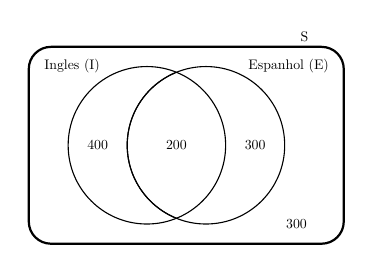
\begin{tikzpicture}
[scale=0.5]
\node [scale=0.5] at (7,5.25) {S};
\draw [ thick,rounded corners=8pt, -] (0,-0) -- (0,5) -- (8,5) -- (8,0) -- cycle;
\node [scale=0.5] at (6.6,4.5) {Espanhol (E)};
\node [scale=0.5] at (1.1,4.5) {Ingles (I)};
\draw (4.5,2.5) circle (2cm);
\node [scale=0.5] at (5.75,2.5) {300};
\node [scale=0.5] at (6.8,0.5) {300};
\clip [draw]  (3,2.5) circle (2cm) ;
\draw [] (4.5,2.5) circle (2cm);
\node [scale=0.5] at (3.75,2.5) {200};
\node [scale=0.5] at (1.75,2.5) {400};
\end{tikzpicture}\end{center}
Logo, a probabilidade de falar espanhol dado que não fala inglês é dada por

\(P(E|\bar{I})=\frac{P(E\cap \bar{I})}{P(\bar{I})}=\frac{300/1200}{600/1200}=\frac{1}{2}.\)

\(17.\) Opção correta: (B)

Observe que o teste terminará na quinta questão se o segundo erro do candidato ocorrer nessa questão. Portanto, para o primeiro erro haverá quatro eventos possíveis, a saber, na primeira ou na segunda ou na terceira ou na quarta questão. Como esses eventos são disjuntos, a probabilidade desejada será dada pela soma das probabilidades desses 4 eventos. Observe também que cada um desses eventos, usando a independência entre questões, ocorre com probabilidade, \(0,2^2\cdot 0,8^3=0,02048\), correspondendo a dois erros e três acertos. Portanto, a resposta é \(4\cdot 0,02048=0,08192\).

\(18.\) Para as seleções sem reposição tem-se o seguinte diagrama de árvore
\begin{center}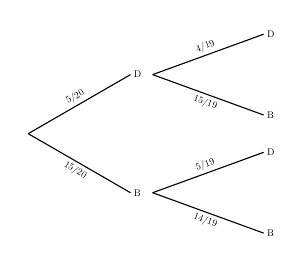
\begin{tikzpicture}
[scale=0.5]
\draw (0,0) -- (30:3) node [right, scale=0.35] {D} node [above, midway, rotate=30, scale=0.35] {5/20};
\draw (0,0) -- (-30:3) node [right, scale=0.35] {B} node [below, midway, rotate=-30, scale=0.35] {15/20};
\draw (3.159807,1.5) -- ++(20:3) node [right, scale=0.35] {D} node [above, midway, rotate=20, scale=0.35] {4/19};
\draw (3.159807,1.5) -- ++(-20:3) node [right, scale=0.35] {B} node [below, midway, rotate=-20, scale=0.35] {15/19};
\draw (3.159807,-1.5) -- ++(20:3) node [right, scale=0.35] {D} node [above, midway, rotate=20, scale=0.35] {5/19};
\draw (3.159807,-1.5) -- ++(-20:3) node [right, scale=0.35] {B} node [below, midway, rotate=-20, scale=0.35] {14/19};
\end{tikzpicture}\end{center}
Assim as respostas são (a) \(\frac{2}{38}\) (b) \(\frac{21}{38}\)  (c) \(\frac{5}{20}\cdot\frac{15}{19}+\frac{15}{20}\cdot\frac{5}{19}=\frac{15}{38}\).

Para as seleções com reposição tem-se o seguinte diagrama de árvore com \(D\) o evento “peça defeituosa e \(B\) peça não defeituosa{}`.
\begin{center}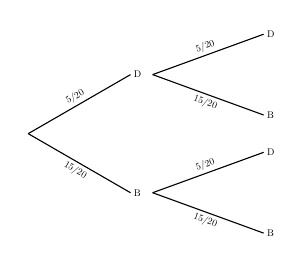
\begin{tikzpicture}
[scale=0.5]
\draw (0,0) -- (30:3) node [right, scale=0.35] {D} node [above, midway, rotate=30, scale=0.35] {5/20};
\draw (0,0) -- (-30:3) node [right, scale=0.35] {B} node [below, midway, rotate=-30, scale=0.35] {15/20};
                                                               \draw (3.159807,1.5) -- ++(20:3) node [right, scale=0.35] {D} node [above, midway, rotate=20, scale=0.35] {5/20};
\draw (3.159807,1.5) -- ++(-20:3) node [right, scale=0.35] {B} node [below, midway, rotate=-20, scale=0.35] {15/20};
\draw (3.159807,-1.5) -- ++(20:3) node [right, scale=0.35] {D} node [above, midway, rotate=20, scale=0.35] {5/20};
\draw (3.159807,-1.5) -- ++(-20:3) node [right, scale=0.35] {B} node [below, midway, rotate=-20, scale=0.35] {15/20};
\end{tikzpicture}\end{center}
Assim as respostas são (a) \(\frac{1}{16}\) (b) \(\frac{9}{16}\)  (c) {}`      Assim as respostas são (a) \(\frac{2}{38}\) (b) \(\frac{21}{38}\)  (c) \(\frac{5}{20}\cdot\frac{15}{20}+\frac{15}{20}\cdot\frac{5}{20}=\frac{6}{16}\).
\end{sphinxadmonition}

